 %%%%%%%%%%%%%%%%%%%%%%%%%%%%%%%%%%%%%%%%%%%%%%%%%%%%%%%%%%%%%%%%%
% \listfiles    % Erstellt eine Liste von allen benutzten Dateien
% zusammen mit ihrer Versionen
% und ggf. einer kurzen Beschreibung
% Sie wird in die log-Datei geschrieben

\documentclass[12pt,a4paper% die Verwendung von DIN-A4-Format ist pflicht!
]{report}
\usepackage[top=2cm, bottom=2.5cm, left=3cm, right=3cm]{geometry}

%notwendige Pakete
\usepackage[english, ngerman]{babel}    % mehrsprachiger Textsatz
% babel: letzte Sprache in Optionen zeigt die Sprache des Dokumentes
% und kann durch den Befehl \selectlanguage{} geaendert werden
% Passen Sie die Optionen des babel-Paketes nach Bedarf an!
\usepackage[utf8]{inputenc}       % Eingabekodierung Parameter latin1 darf 
%ge�ndert werden
\usepackage[T1]{fontenc}                % Schriftenkodierung
\usepackage{graphicx}                       % zum Einbinden von Grafiken
\usepackage{lmodern}                        % Ersatz fuer Computer Modern-Schriften
                                                                % zum besseren Aussehen am Bildschirm

\usepackage{amsmath}
\usepackage{amsfonts}
\usepackage{amssymb}  % mathe-structures
\usepackage{float}
\usepackage{listings} % quellcode

\usepackage{setspace} % Zwischenraum \vspace{length}
\usepackage{threeparttable} % Fußnoten in Tabellen 
\usepackage{multirow} % Text von mehreren Spalten in Tabellen in eine Spalte 
%schreiben
\usepackage{subfigure}

%-Eingabe der Metadaten des Titelblattes--------------------------

%-Daten des Autors / Authors Data---------------------------------

\newcommand{\dcauthorpre}{~} 
\newcommand{\dcauthorsurname}{Kullmann} 
\newcommand{\dcauthorname}{Richard} 
\newcommand{\dcauthoradd}{geboren am 17.07.1996 in Berlin-Pankow}

%-Titel und Untertitel / Title and subtitle-----------------------

\newcommand{\dctitle}{Giant Diffusion in two-dimensional Neuron Models} 
\newcommand{\dcsubtitle}{~}  
% Falls dcsubtitle NICHT verwendet werden soll, {\dcsubtitle}{~} eingeben.

%-Eingabe der Betreuuernahmen / Names of the consultants---------

\newcommand{\dcconsulta}{~} 
\newcommand{\dcconsultb}{~} 
\newcommand{\dcconsultc}{~} 

%-Eingabe der Gutachternamen / Names of the approvals-------------

\newcommand{\dcapprovala}{Prof. Dr. Benjamin Lindner} 
\newcommand{\dcapprovalb}{Prof. Dr. Igor Sokolov} 
\newcommand{\dcapprovalc}{~} 

%-Information zur Universitaet------------------------------------

\newcommand{\dcdegree}{Master of Science\\(M. Sc.)} 
\newcommand{\dcsubject}{Physik} 
\newcommand{\dcfaculty}{Mathematisch-Naturwissenschaftlichen Fakult\"at I}
\newcommand{\dcinstitute}{Institut f\"ur Physik}
\newcommand{\dcuniversity}{Humboldt-Universit\"at zu Berlin}
\newcommand{\dcdean}{Prof. Dr. sc. Heinz  M\"uller}
\newcommand{\dcpresident}{Prof. Dr. Dr. h.c. Wilhelm Schulz}

%-Pruefungsdaten: eingereicht und mdl. Pruefung-------------------
%-data of submission and oral exam--------------------------------

\newcommand{\dcdatesubmitted}{5. Juni 2020} %auch wenn nicht auf dem 
%Titelblatt, bitte erf�llen!
\newcommand{\dcdateexam}{2. Juli 1999} 


% Folgende Zeile bitte nicht aendern!
\newcommand{\dckeywordsde}{\vfill \raggedright {\textbf{Schlagw\"orter:}}\\ \dckeydea, \dckeydeb, \dckeydec, \dckeyded \\}

%-englische Schlagwoerter / english keywords----------------------

\newcommand{\dckeyena}{Giant Diffusion}
\newcommand{\dckeyenb}{Two-Dimensional Neuron Models}
\newcommand{\dckeyenc}{Bistability}
\newcommand{\dckeyend}{Signal-to-Noise Ratio}

% Folgende Zeile bitte nicht aendern!
\newcommand{\dckeywordsen}{\vfill \raggedright {\textbf{Keywords:}}\\ \dckeyena, \dckeyenb, \dckeyenc, \dckeyend \\}

\newcommand{\dcpdfsubject}{Dissertation}                          % Bitte ALLE Angaben 
%erfüllen!
\usepackage{ifpdf}

\ifpdf
%%das kann man benutzen, wenn man andere Formate benutzen will
%\DeclareGraphicsExtensions{{.pdf}}   %Endung der Grafiken, wenn nicht pdf
% die folgenden Angaben sind im PDF unter Datei | Dokumenteigenschaften 
% in Acrobat / Acrobat Reader sichtbar
% Aendern Sie bitte die Daten, wo noetig!
\usepackage[%
	pdftitle={\dctitle},
	pdfauthor={\dcauthorsurname\ \dcauthorname},
	pdfsubject={\dcpdfsubject}, % optional
	pdfkeywords={\dckeydea, \dckeydeb, \dckeydec, \dckeyded},
	pdfpagemode=UseOutlines,
  colorlinks=true,					% bitte nicht �ndern!
	linkcolor=black,					% bitte nicht �ndern!
	filecolor=black,					% bitte nicht �ndern!
	urlcolor=black,						% bitte nicht �ndern!
	citecolor=black,					% bitte nicht �ndern!
	pdftex=true,              % bitte nicht �ndern!
	plainpages=false,         % bitte nicht �ndern!
	hypertexnames=false,      % bitte nicht �ndern!
	pdfpagelabels=true,       % bitte nicht �ndern!
	hyperindex=true]{hyperref}% bitte nicht �ndern!
\else
  % hier kann mann eventuelle Befehle umdefinieren
  % die nur f�r pdfLaTeX vorgesehen sind
  % und das richtige Kompilieren durch den normalen LaTeX verhindern
	\newcommand{\texorpdfstring}[1]{#1}
\fi

%-Eigene Trennregeln*---------------------------------------------

% % Tragen Sie Ihre eigenen Trennregel ein:
\hyphenation{Bei-spiel, �-ko-lo-gie}

%-zusaetzliche Kommandos*-----------------------------------------

\newcommand{\rl}[1]	{\left({#1}\right)}
\newcommand{\Bra}[1] {\left\langle {#1} \right|}
\newcommand{\Ket}[1]{\left|{#1}\right\rangle}
\newcommand{\braket}[2]{\left\langle #1 | #2 \right\rangle}
\newcommand{\Op}[1]{\hat{\text{#1}}}
\newcommand{\opi}[2]{\hat{\text{#1}}_{\text{#2}}}
\newcommand{\opij}[3]{\hat{\text{#1}}_{#2,#3}}
\newcommand{\DEL}{\partial}

\graphicspath{{images/}}

%-Dokument--------------------------------------------------------

\begin{document}

% Es muss zitiert werden können! Im Vorspann roemisch,
% Im Hauptteil benutzt man arabische Nummerierung.
\pagenumbering{roman}

%-Titelblatt------------------------------------------------------

%----------Generierung der Titelseite-----bitte nicht ver�ndern!--------------------


\author{von \\ \dcauthorpre\ \dcauthorname\ \dcauthorsurname\ \\ \dcauthoradd}

%----------
\title{ \vspace{-2cm}\dctitle \\ 
\vspace{0.5cm}
\large{\dcsubtitle} \\ 
\vspace{0.5cm} {\Large{MASTERARBEIT}}\\ 
\vspace{0.5cm} \large{zur Erlangung des akademischen Grades \\ 
\dcdegree\\ im Fach \dcsubject \\\vspace{0.5cm}

\includegraphics[width=6cm]{husiegel}\\ 
\vspace{0.5cm} eingereicht an der \\ 
\dcfaculty \\ 
\dcinstitute\\
\dcuniversity \\}}
%-----------------
\date{\vspace{2.5cm}
%\raggedright{
%Pr\"asident der Humboldt-Universit\"at zu Berlin:\\
%\dcpresident \vspace{-0.3cm}
%}\vspace{0.5cm}\\
%
%\raggedright{
%Dekan der \dcfaculty:\\
%\dcdean \vspace{-0.3cm}
%}\vspace{0.5cm}\\
%
% auskommentiert weil nicht standard
\raggedright{
Gutachter:
\begin{enumerate} 
\item{\it\dcapprovala} \vspace{-0.3cm}
\item{\it\dcapprovalb} \vspace{-0.3cm}
%\item{\it\dcapprovalc} \vspace{-0.3cm}
\end{enumerate}} \vspace{0.5cm}
%\raggedright{
%Betreuung:
%\begin{enumerate} 
%\item{\it\dcconsulta} \vspace{-0.2cm}
%\item{\it\dcconsultb} \vspace{-0.2cm}
%\end{enumerate}} \vspace{0.5cm}
%-----------------
\raggedright{
\begin{tabular}{lll}
eingereicht am: &  &\it\dcdatesubmitted\\ % wenn nicht in der Pr�fungsordnung, die Zeile bitte auskommentieren
%Tag der m\"undlichen Pr\"ufung: & & \dcdateexam
\end{tabular}}\\ 
}
%-------------------------------------                         % Bitte KEINE �nderungen 
%vornehmen!
\maketitle


%-Zusammenfassung / Abstract*-------------------------------------

%-englische-Zusammenfassung---------------------------------------

%\selectlanguage{english}

%\begin{abstract}
%\setcounter{page}{2} % Nach Bedarf anpassen!
%Here is the english abstract.\\
% hier werden die englische Schlagw�rter aus Metadaten �bernommen
%\dckeywordsen				
%\end{abstract}

%-deutsche Zusammenfassung----------------------------------------

%\selectlanguage{german}

\begin{abstract}
\setcounter{page}{2} % Nach Bedarf anpassen!
The emerging field of magnetometry based on NV centers opens a variety of new experimental perspectives, including the imaging of single nuclear spins on the nanoscale. However, in order to achieve exceptionally long NV electron spin coherence times and high sensitivities, the NV spin needs to be decoupled from unwanted interactions with the environment. This can be accomplished with dynamical decoupling sequences.
\\
During the work for this thesis, multiple dynamical decoupling protocols were implemented and tested on NV centers in bulk diamond and nanodiamond. 
\\
The theoretical part covers general NV properties before treating the behaviour of a free electron spin and finally applying this on the NV center. Then, the effect of different decoupling protocols are discussed. After that, the structure and concept of the setup will be explained. In the final part, the measurements will be presented. The execution of the decoupling sequences will be demonstrated and the data will be used to extract the spectral density function of the environment.
\\
It was shown that all implemented dynamical decoupling sequences could enhance the coherence time. It was demonstrated that CPMG outperforms the other sequences on the given setup, achieving an improvement of up to a factor of 200 in the bulk diamond and 50 in nanodiamond. Finally, the examination of the spectral density functions of the spin bath gave a deeper insight in its coupling strength to the NV and its internal dynamics.\\
In the future, the limitations of the sequences will be further explored and other decoupling protocols will be tested. In addition to that, a better time and phase control has to be accomplished. These efforts will eventually lead to sensitivities high enough to detect small spin ensembles and even single molecular spins.
% hier werden die deutsche Schlagw�rter aus Metadaten �bernommen
%\dckeywordsde
\end{abstract}
\thispagestyle{empty}

\selectlanguage{ngerman}               % Bitte an die Sprache denken!!!
\setcounter{page}{3}                   %   Bitte an die Seitenzahl denken!!!

%-Widmung*--------------------------------------------------------

%\chapter*{Widmung}
Hier folgt dann eine Widmung.

%-Inhaltsverzeichnis----------------------------------------------

\tableofcontents
\pagebreak

\listoffigures
\pagebreak

\listoftables
\pagebreak

%-Hauptteil-------------------------------------------------------

\pagenumbering{arabic}
\pagestyle{myheadings}                  % bzw. ist fancyhdr zu benutzten

%-Kapitel---------------------------------------------------------

% part ist optional, bitte ggf. löschen
% \part{Teil1}

%\chapter{Einleitung}

Nach der ersten experimentellen Realisierung von Bose-Einstein-Kondensaten 
(\textit{engl.: Bose-Einstein-Condensate}, kurz BEC) im Jahre 1995 
(\cite{av:m2},\cite{av:m3},\cite{av:m4}), ca. 70 Jahre nach der theoretischen 
Vorhersage und dem darauf 
folgenden Nobelpreis \cite{av:m1} im Jahre 2001 hat sich ein neues 
Forschungsgebiet der Atom- und Molekülphysik sowie in der Quantenoptik 
eröffnet. 

BECs sind makroskopische Quantenobjekte. Sie bestehen aus 
ultrakalten, 
neutralen, bosonischen Atomen, die quantenmechanisch überwiegend den 
Grundzustand des Systems besiedeln. Dabei ist die Wellenfunktion eines 
einzelnen Teilchens stark delokalisiert.  

Eine sehr erfolgreiche Methode BECs theoretisch zu beschreiben, liefert die 
"Meanfield-Theorie"\ bei der angenommen wird, dass sich der quantenmechanische 
Zustand des Mehrteilchensystems durch eine einzige effektive Wellenfunktion 
beschreiben lässt. Durch iterative Verfahren kann so nicht 
nur die Energie, 
sondern auch die Form des BECs abgeschätzt werden. Da neutrale Atome im 
ultrakalten Regime, das heißt im Mikro- bis Nanokelvin 
Bereich, 
nur 
auf einer sehr 
kurzen Distanz wechselwirken (s-Wellen-Streuung), stellt das sogenannte 
$\delta$-Pseudopotential eine gute Näherung dar. Es entspricht einer 
Kontaktwechselwirkung mit effektiver Streulänge.

Will man darüber hinaus eine genauere Berechnung durchführen, bietet sich 
eine Konfigurationswechselwirkungsrechnung (\textit{engl.: Configuration 
Interaction}, kurz CI) an. Dabei stellt man schnell 
fest, dass bei klassischen BECs mit einer Teilchenzahl in der Größenordnung 
von $10^{5}$ (vergleiche mit \cite{av:m2}) eine zu große Anzahl an 
Konfigurationen im System vorhanden sind und so 
die Berechnung fast unmöglich scheint.

Seit 2011 ist es möglich, einzelne Atome in 
optischen Dipol-Fallen, das heißt, mit Lasern zu 
halten \cite{av:7a} und diese zu untersuchen. Weiterhin gibt es die Variante, 
sogenannte optische Gitter zu erstellen, womit BECs sogar 3d-periodisch 
angeordnet werden können (siehe u.a. in \cite{phdthesis:Schneider}, 
\cite{phdthesis:sala}). Daher kann für solche sehr kleinen Systeme dieser 
Ansatz wieder verfolgt werden.

Das Problem ist nun jedoch, dass eine genauere Berechnung von BECs mithilfe 
des Deltapotentials im Rahmen einer CI-Rechnung in 3d nicht möglich ist. 
\cite{av:1b} zeigt, dass die Energie hierbei nicht konvergiert. Für immer 
größere Konfigurationen entsteht eine immer höhere Energie des Systems.

Es gibt zwei Herangehensweisen, um mit einer solchen Divergenz umzugehen. Zum 
einen kann versucht werden, die Berechnung zu renormieren, das heißt die 
Unendlichkeit durch eine  Re-Definition von Operatoren zu umgehen. Ein solches 
Vorgehen ist unter anderem in \cite{phdthesis:sala} erfolglos versucht worden. 
%
Ein anderer Weg wäre es, ein realistischeres Wechelwirkungspotential zu 
benutzen. Dieses setzt sich prinzipiell aus zwei Teilen 
zusammen: Einen 
abstoßenden Part, der verhindert, dass sich zwei Teilchen am exakt selben Ort 
befinde und einen anziehenden Part, der durch die 
Van-der-Waals 
Wechselwirkung beschrieben wird. Wechselwirkungspotentiale sind sehr 
kurzreichweitig.  Auf der anderen Seite werden BECs in optischen Fallen 
gehalten, die in erster Näherung durch ein harmonisches Potential beschrieben 
werden können. Das Fallenpotential ist auf Grund der makroskopischen Größe der 
Apparatur langreichweitig gegenüber der Ausdehnung des BECs.  Beide Potentiale 
sollen bei einer genaueren Berechnung berücksichtigt werden, 
was auf Grund der 
unterschiedlichen Skalen der Ausdehnung die Rechnung erschwert.

Es entstehen schwer zu berechnende Wechselwirkungsintegrale, 
die prinzipiell von 6 Koordinaten abhängen und im Allgemeinen nicht separieren.

Für das Zweiteilchenproblem in einem optischen Gitter hat man in 
\cite{phdthesis:sergey} eine analytische Lösung in Relativ- und 
Schwerpunktskoordinaten gefunden. Dieses Vorgehen kann jedoch für mehr als zwei 
Teilchen nicht mehr angewendet werden.

Im Kontext der Elektronenstrukturrechnungen von Molekülen stößt man auch auf 
solche sechsdimensionalen Wechselwirkungsintegrale. 2015 wird 
in der Arbeit 
\cite{av:1a} ein Vorgehen präsentiert, wie eine sehr allgemeine Klasse der 
Integrale erst vereinfacht und anschließend über eine Schar 
an Basisintegralen 
berechnet werden kann. \\

Ziel dieser Arbeit soll es also sein, den vorgestellten 
Algorithmus zu 
überprüfen, zu implementieren und die Anwendbarkeit auf die Berechnung von 
ultrakalten Gasen mittels CI abzuschätzen. Damit wäre ein neuer Zugang zu einer 
genaueren Berechnung und damit ein tieferes Verständnis von BECs möglich. \\


Zukünftig können BECs  in vielen Anwendungsbereichen zum Einsatz kommen. 
Vorstellbar wären Bereiche wie Quantencomputer, Quantensimulatoren oder auch 
Quantensensoren. Einige Ideen zur Nutzung von BECs im Rahmen von 
Quantencomputern können in \cite{phdthesis:Schneider} 
gefunden werden. Weiterhin 
zeigt \cite{av:m5} ein Beispiel der Anwendung für Quantensensoren.
Letztere versprechen äußerst präzise Messungen auf der Skala einzelner Atome.
Um zum Beispiel Quantensensoren zu realisieren bzw. zu 
verbessern, muss es auch 
theoretische Grundlagen und präzise Vorhersagen bzgl. des Verhaltens von BECs 
auf einer sehr kleinen Skalierung und mit hoher Genauigkeit geben.\\
\ \\[1cm]
Demzufolge erklärt diese Arbeit zunächst das betrachtete System und die 
theoretische Grundlage erklärt, worauf eine CI Rechnung 
basiert. Anschließend 
wird der Algorithmus zur Berechnung von sechsedimensionalen Integralen 
vorgestellt und an das hier betrachtete Problem angepasst. In Kapitel 3 wird 
die Implementierung erläutert und getestet. Danach wird ein 
Fazit gegeben 
und ein Ausblick auf die nächsten Schritte dargestellt.

\chapter{Einleitung}

Nach der ersten experimentellen Realisierung von Bose-Einstein-Kondensaten 
(\textit{engl.: Bose-Einstein-Condensate}, kurz BEC) im Jahre 1995 
(\cite{av:m2},\cite{av:m3},\cite{av:m4}), ca. 70 Jahre nach der theoretischen 
Vorhersage und dem darauf 
folgenden Nobelpreis \cite{av:m1} im Jahre 2001 hat sich ein neues 
Forschungsgebiet der Atom- und Molekülphysik sowie in der Quantenoptik 
eröffnet. 

BECs sind makroskopische Quantenobjekte. Sie bestehen aus 
ultrakalten, 
neutralen, bosonischen Atomen, die quantenmechanisch überwiegend den 
Grundzustand des Systems besiedeln. Dabei ist die Wellenfunktion eines 
einzelnen Teilchens stark delokalisiert.  

Eine sehr erfolgreiche Methode BECs theoretisch zu beschreiben, liefert die 
"Meanfield-Theorie"\ bei der angenommen wird, dass sich der quantenmechanische 
Zustand des Mehrteilchensystems durch eine einzige effektive Wellenfunktion 
beschreiben lässt. Durch iterative Verfahren kann so nicht 
nur die Energie, 
sondern auch die Form des BECs abgeschätzt werden. Da neutrale Atome im 
ultrakalten Regime, das heißt im Mikro- bis Nanokelvin 
Bereich, 
nur 
auf einer sehr 
kurzen Distanz wechselwirken (s-Wellen-Streuung), stellt das sogenannte 
$\delta$-Pseudopotential eine gute Näherung dar. Es entspricht einer 
Kontaktwechselwirkung mit effektiver Streulänge.

Will man darüber hinaus eine genauere Berechnung durchführen, bietet sich 
eine Konfigurationswechselwirkungsrechnung (\textit{engl.: Configuration 
Interaction}, kurz CI) an. Dabei stellt man schnell 
fest, dass bei klassischen BECs mit einer Teilchenzahl in der Größenordnung 
von $10^{5}$ (vergleiche mit \cite{av:m2}) eine zu große Anzahl an 
Konfigurationen im System vorhanden sind und so 
die Berechnung fast unmöglich scheint.

Seit 2011 ist es möglich, einzelne Atome in 
optischen Dipol-Fallen, das heißt, mit Lasern zu 
halten \cite{av:7a} und diese zu untersuchen. Weiterhin gibt es die Variante, 
sogenannte optische Gitter zu erstellen, womit BECs sogar 3d-periodisch 
angeordnet werden können (siehe u.a. in \cite{phdthesis:Schneider}, 
\cite{phdthesis:sala}). Daher kann für solche sehr kleinen Systeme dieser 
Ansatz wieder verfolgt werden.

Das Problem ist nun jedoch, dass eine genauere Berechnung von BECs mithilfe 
des Deltapotentials im Rahmen einer CI-Rechnung in 3d nicht möglich ist. 
\cite{av:1b} zeigt, dass die Energie hierbei nicht konvergiert. Für immer 
größere Konfigurationen entsteht eine immer höhere Energie des Systems.

Es gibt zwei Herangehensweisen, um mit einer solchen Divergenz umzugehen. Zum 
einen kann versucht werden, die Berechnung zu renormieren, das heißt die 
Unendlichkeit durch eine  Re-Definition von Operatoren zu umgehen. Ein solches 
Vorgehen ist unter anderem in \cite{phdthesis:sala} erfolglos versucht worden. 
%
Ein anderer Weg wäre es, ein realistischeres Wechelwirkungspotential zu 
benutzen. Dieses setzt sich prinzipiell aus zwei Teilen 
zusammen: Einen 
abstoßenden Part, der verhindert, dass sich zwei Teilchen am exakt selben Ort 
befinde und einen anziehenden Part, der durch die 
Van-der-Waals 
Wechselwirkung beschrieben wird. Wechselwirkungspotentiale sind sehr 
kurzreichweitig.  Auf der anderen Seite werden BECs in optischen Fallen 
gehalten, die in erster Näherung durch ein harmonisches Potential beschrieben 
werden können. Das Fallenpotential ist auf Grund der makroskopischen Größe der 
Apparatur langreichweitig gegenüber der Ausdehnung des BECs.  Beide Potentiale 
sollen bei einer genaueren Berechnung berücksichtigt werden, 
was auf Grund der 
unterschiedlichen Skalen der Ausdehnung die Rechnung erschwert.

Es entstehen schwer zu berechnende Wechselwirkungsintegrale, 
die prinzipiell von 6 Koordinaten abhängen und im Allgemeinen nicht separieren.

Für das Zweiteilchenproblem in einem optischen Gitter hat man in 
\cite{phdthesis:sergey} eine analytische Lösung in Relativ- und 
Schwerpunktskoordinaten gefunden. Dieses Vorgehen kann jedoch für mehr als zwei 
Teilchen nicht mehr angewendet werden.

Im Kontext der Elektronenstrukturrechnungen von Molekülen stößt man auch auf 
solche sechsdimensionalen Wechselwirkungsintegrale. 2015 wird 
in der Arbeit 
\cite{av:1a} ein Vorgehen präsentiert, wie eine sehr allgemeine Klasse der 
Integrale erst vereinfacht und anschließend über eine Schar 
an Basisintegralen 
berechnet werden kann. \\

Ziel dieser Arbeit soll es also sein, den vorgestellten 
Algorithmus zu 
überprüfen, zu implementieren und die Anwendbarkeit auf die Berechnung von 
ultrakalten Gasen mittels CI abzuschätzen. Damit wäre ein neuer Zugang zu einer 
genaueren Berechnung und damit ein tieferes Verständnis von BECs möglich. \\


Zukünftig können BECs  in vielen Anwendungsbereichen zum Einsatz kommen. 
Vorstellbar wären Bereiche wie Quantencomputer, Quantensimulatoren oder auch 
Quantensensoren. Einige Ideen zur Nutzung von BECs im Rahmen von 
Quantencomputern können in \cite{phdthesis:Schneider} 
gefunden werden. Weiterhin 
zeigt \cite{av:m5} ein Beispiel der Anwendung für Quantensensoren.
Letztere versprechen äußerst präzise Messungen auf der Skala einzelner Atome.
Um zum Beispiel Quantensensoren zu realisieren bzw. zu 
verbessern, muss es auch 
theoretische Grundlagen und präzise Vorhersagen bzgl. des Verhaltens von BECs 
auf einer sehr kleinen Skalierung und mit hoher Genauigkeit geben.\\
\ \\[1cm]
Demzufolge erklärt diese Arbeit zunächst das betrachtete System und die 
theoretische Grundlage erklärt, worauf eine CI Rechnung 
basiert. Anschließend 
wird der Algorithmus zur Berechnung von sechsedimensionalen Integralen 
vorgestellt und an das hier betrachtete Problem angepasst. In Kapitel 3 wird 
die Implementierung erläutert und getestet. Danach wird ein 
Fazit gegeben 
und ein Ausblick auf die nächsten Schritte dargestellt.

%\chapter{Theorie}
%
%
%\section{Theoretische Grundlagen}
%
Im Rahmen dieser Arbeit werden, wenn nicht anders gekennzeichnet, atomare
Einheiten verwendet. Das bedeutet, Energien werden in Einheiten von \\ 1 $E_h$ 
(Hartree) =  2 Rydberg $\approx$ 27.21 eV, Massen in 1 $m_e$, Strecken in 1
$a_0$ und Ladungen in Einheiten von 1 $e$ angegeben.
%
%
%
\section{System}\label{sec:System}
%
Untersucht wird ein ultrakaltes Zweiteilchensystem.
Stellvertretend für andere Systeme kann das bosonische Zweiatomsystem 
Li$^7$Li$^7$ betrachtet werden. Der Hamilton-Operator 
%
\begin{align}\label{eq:kernHam1}
	\Op{H}=\sum_{i=1}^{2}\Op{T}_{K_i}
		+\sum_{i=1}^{2} \Op{V}_{\text{F}}(\textbf{r}_i)
		+\Op{U}(|\textbf{r}_1-\textbf{r}_2|) 
\end{align} 
% 
beschreibt mithilfe der nicht-relativistischen, stationären Schrödingergleichung
%
\begin{align}\label{eq:algSg1}
	\Op{H}\Ket{\psi} = \text{E} \Ket{\psi}
\end{align}
%
das System. 
$\Op{T}_{K_j}=\frac{1}{2\text{M}}\nabla^2_{r_j}$\
ist der 
Kinetische-Energieoperator des jeweiligen Kerns. $\Op{V}_\text{F}$ beschreibt 
ein
Fallenpotential, welches in dieser Arbeit als isotrop und harmonisch angenommen 
wird, das 
heißt 
%
\begin{align}
\Op{V}_\text{F}(\text{r}_i) = \frac{1}{2}\,\text{M}\,\omega^2\, 
\textbf{r}^2_i=\frac{1}{2}\,\text{M}\,\omega^2 \rl{ \, \text{x}^2_i + 
\text{y}^2_i + 
\text{z}^2_i\, } \quad.
\end{align}
%. 
$\Op{U}$  ist eine aus 
Elektronenstrukturrechnung oder Experimenten bekanntes oder motiviertes  
effektives Wechselwirkungspotential. Für Li$^7$Li$^7$ ist in 
\cite{phdthesis:sergey} und den darin enthaltenden Referenzen ein 
solches Potential stückweise zusammengestellt worden, das 
in Grafik 
\ref{pic:NP} dargestellt ist. \\
 
%
%\begin{figure}[t] \centering
%	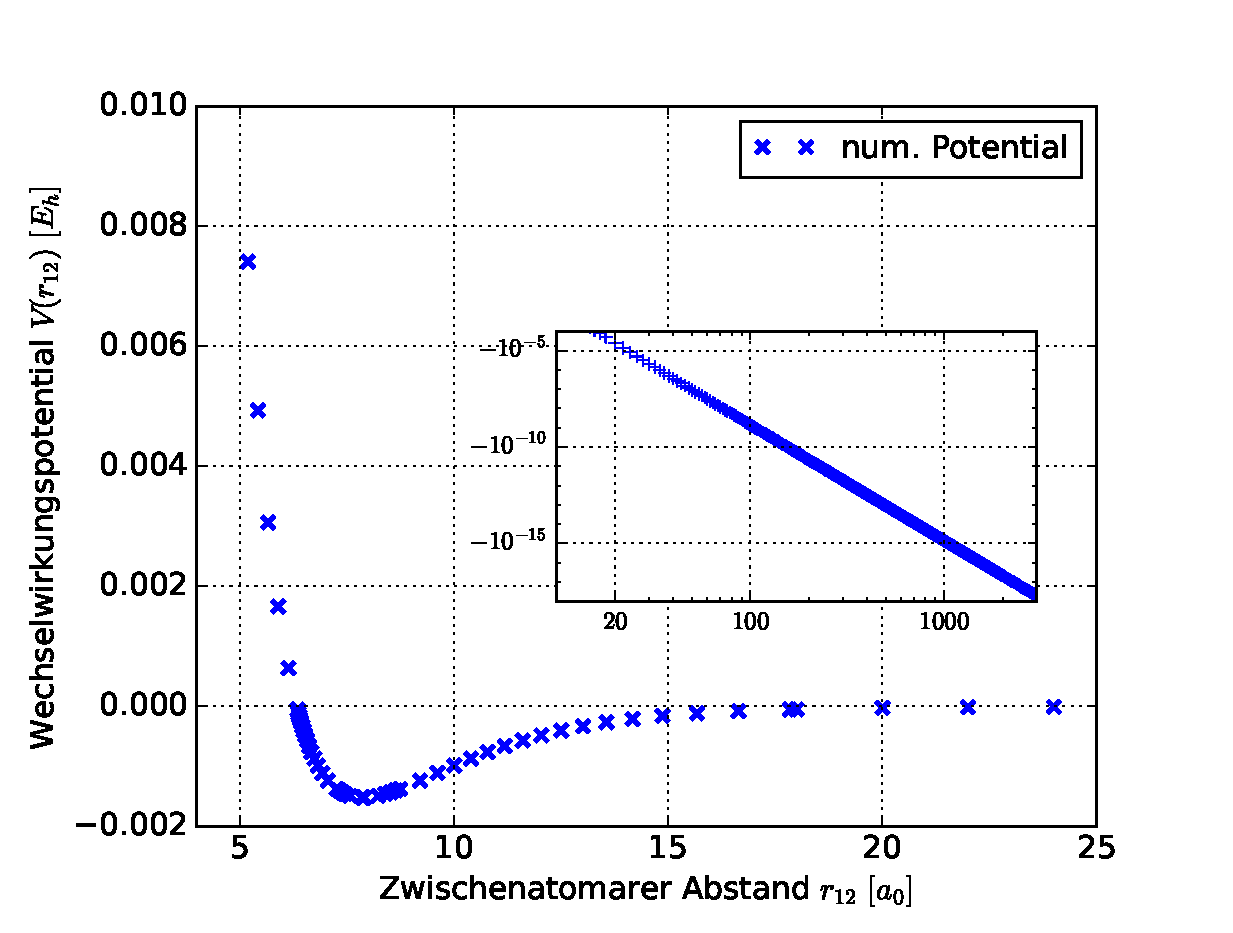
\includegraphics[scale=0.65]{NP.eps}
%	%	\vspace*{-10mm}
%	\caption{Dargestellt ist ein numerisches 
%	Wechselwirkungspotential (gekreuzt) eines 
%		angeregten Tripletzustandes des 
%		$^7$Li$^7$Li Systems.}
%	%\vspace{2mm} %\hrule 
%	\label{pic:NP} 
%\end{figure}
%
Eine mögliche experimentelle Vorlage für ein Zweiatomsystem ist 2011  
realisiert worden \cite{av:7a}.
 Hier handelt es sich um eine
optische Dipolfalle, welche in erster Ordnung auch durch ein quadratisches
Potential beschrieben werden kann  \cite{phdthesis:sala}.  Die ermittelte 
effektive Fallenfrequenz liegt in der Größenordnung von
$10^{4}$ Hz $\approx$ $10^{-13}\ \omega_0$ in atomaren Einheiten. 
% 
\pagebreak
%
%
%
\section{Konfigurationswechselwirkungsrechnung}
%
Da \ref{eq:algSg1} im Allgemeinen nur schwer zu lösen ist, kann nun eine aus der
Quantenchemie (siehe z.B. \cite{b:3a}) bekannte Lösungsmethode herangezogen 
werden:
die Konfigurationswechselwirkungsrechnung (CI). Dazu wird die Wellenfunktion in 
einer endlichen Basis $\Ket{\psi_n}$  
entwickelt    
%
\begin{align}\label{eq:CI-Ansatz}
	\Ket{\psi} \approx \sum_n^N c_n \Ket{\psi_n} \quad.
\end{align}
%
Anschließend wird $\Bra{\psi_i}$ an Gleichung \ref{eq:algSg1} multipliziert. Es 
entsteht das 
Eigenwertproblem
%
\begin{align}\label{eq:EWP}
	\textbf{H}\textbf{c}=E\cdot \textbf{S}\textbf{c}
\end{align}
%
mit 
%
\begin{align}\label{eq:Matrixelemente}
	H_{ij}&=\Bra{\psi_i} \Op{H}\Ket{\psi_j}\\
	S_{ij}&=\braket{\psi_i}{\psi_j} \quad .
\end{align}
%
Wäre die Entwicklung \ref{eq:CI-Ansatz} unendlich und der Basissatz vollständig,
wäre dieser Ansatz exakt. Die Matrix \textbf{S} beinhaltet den sogenannten 
Überlapp der Basisfunktionen. Sind diese orthogonal, so entspricht \textbf{S} 
einer Einheitsmatrix.  Weiterhin wird angenommen, dass sich die 
Basiswellenfunktionen als Produkt der 
Einteilchenwellenfunktionen
beschreiben lassen.

Um die Matrixelemente zu berechnen, müssen 
sechsdimensionale Integrale gelöst werden.%TODO der Satz kommt aus dem nichts, 
%vlt weg lassen
%
%
%
\section{Methodik}
%
%
%
\subsection{Ansatz}
%
Als Ansatz für die oben erwähnten Basisfunktionen werden sogenannte Kartesische-
Gauß-Funktionen bzw. "gaussian-typ orbitals"\ kurz GTOs verwendet. Dieser Ansatz
entstammt der Arbeit von Boys in den 1950er Jahren \cite{av:5a} und ist heute
Standard bei der Elektronenstrukturrechnung (siehe z.B.: \cite{b:3a},
\cite{b:2a}). Die Wellenfunktion in der Ortsdarstellung wird 
also in
Termen von 
%
\begin{align}
\braket{\textbf{r}}{\psi_n}=\psi_n^a(\textbf{r}_1)\cdot\psi_n^c(\textbf{r}_2)
\end{align}
%
mit je
%
\begin{align}\nonumber
\psi_n^a(i,k,m,a,\textbf{A},\textbf{r})&=N_{ikm}(a)\cdot (x-A_x)^i\cdot 
(y-A_y)^k\cdot (z-A_z)^m\  \cdot\\ \label{eq:Produktansatz}
& \qquad \cdot \exp\rl{-a\cdot 
	\rl{(x-A_x)^2+(y-A_y)^2+(z-A_z)^2}}\\\nonumber
%
&= N\cdot x_A^iy_A^kz_A^m\cdot e^{-a r_A^2}\\\nonumber
&= \psi_n^a(\textbf{r})
\end{align}
%
entwickelt. $N$ ist ein Normierungsfaktor und lässt sich mithilfe von 
%
\begin{align}\label{eq:NORM}
	N_{ikm}(a)=\rl{\frac{2a}{\pi}}^\frac{3}{4}\frac{(4a)^\frac{i+k+m}{2}}{\sqrt{(2i-1)!!\cdot(2k-1)!!\cdot(2m-1)!!}}
\end{align}
%
berechnen (vgl. \cite{av:2a}), wobei dieser auch weggelassen werden kann, wobei 
man dann von nicht normierten GTOs spricht.\ \textbf{A} ist 
das 
Zentrum der Gauß-Funktion. Die natürlichen Zahlen ($i,k,m$) geben das 
assoziierte Orbital an. So entspricht zum Beispiel das Tupel (0,0,0) einem 
s-Orbital und (1,0,0) einem p-Orbital in x-Richtung.\\
Um die Matrixelemente \ref{eq:Matrixelemente} ermitteln zu können, müssen 
Einteilchenintegrale
%
\begin{align}\label{eq:1T-Integrale}
\Bra{\psi_i}\Op{O}(\textbf{r}_1)\Ket{\psi_j}  = 
\int  d\textbf{r}_1 
(\psi_i^{a}(\textbf{r}_1) )^*
f(r_1) 
\psi_j^b(\textbf{r}_1)
\end{align}
%
und Zweiteilchenintegrale des Typs
%
\begin{align}\label{eq:2T-Integrale}
I=\Bra{\psi_i}\Op{O}(|\textbf{r}_1-\textbf{r}_2|)\Ket{\psi_j} = \int 
\int\ 
d\textbf{r}_1\ d\textbf{r}_1 
(\psi_i^a(\textbf{r}_1)\psi_i^c(\textbf{r}_2))^* f_{12}(r_{12}) 
\psi_j^b(\textbf{r}_1)\psi_j^d(\textbf{r}_2)
\end{align}
%
zu verschiedenen Operatoren $\Op{O}$ bzw. Funktionen $f$ berechnet werden. Für 
obere Einteilchenintegrale \ref{eq:1T-Integrale} gibt es bereits Algorithmen, 
die effizient implementiert werden können. Die Zweiteilchenintegrale stellen 
dagegen einen größeren Rechenaufwand dar. Anzumerken ist hier, dass die in 
\ref{eq:2T-Integrale} einzusetzenden GTOs prinzipiell unterschiedliche 
Zentren 
haben können. Man spricht hierbei auch von einem 4-Zentrenintegral über GTOs.
%
%
%
\subsection{Berechnung von Zweiteilchenintegralen}\label{sec:Algorithmus}
%
Der in diesem Kapitel vorgestellte Algorithmus entstammt der Veröffentlichung 
\cite{av:1a}. Anders als in dieser Arbeit wird er dort zur Berechnung von 
Zweielektronenintegralen im Rahmen von Elektronenstrukturrechnungen an 
Molekülen verwendet. Weiterhin werden sechs spezielle Fälle für den Integranten 
dargestellt. Für diese Arbeit reicht es aus, den dritten Fall 
(kernal function 3, $k_3(r_{12})$) zu betrachten.\\ 
%
Zur Ableitung des Algorithmus werden vier Schritte der Umformung des Integrals 
vorgenommen. 
%
%
%
\subsubsection{McMurchie-Davidson Schema}
%
Im Abschnitt II.B. von \cite{av:1a} folgt man dem McMurchie-Davidson Schema. 
Dieses entstammt der Arbeit \cite{av:2a} und nutzt aus, dass sich ein Produkt 
aus je zwei Gauß-Funktionen um die Punkte \textbf{A} bzw. \textbf{B} als neue 
Gauß-Funktion 
um einen Punkt \textbf{P} auf der Strecke $\overline{\textbf{AB}}$ schreiben 
lassen. In Abbildung \ref{pic:1d_GTO} ist eine eindimensionale Darstellung 
eines solchen Produkts dargestellt. 
%
%\begin{figure}[H] \centering
%	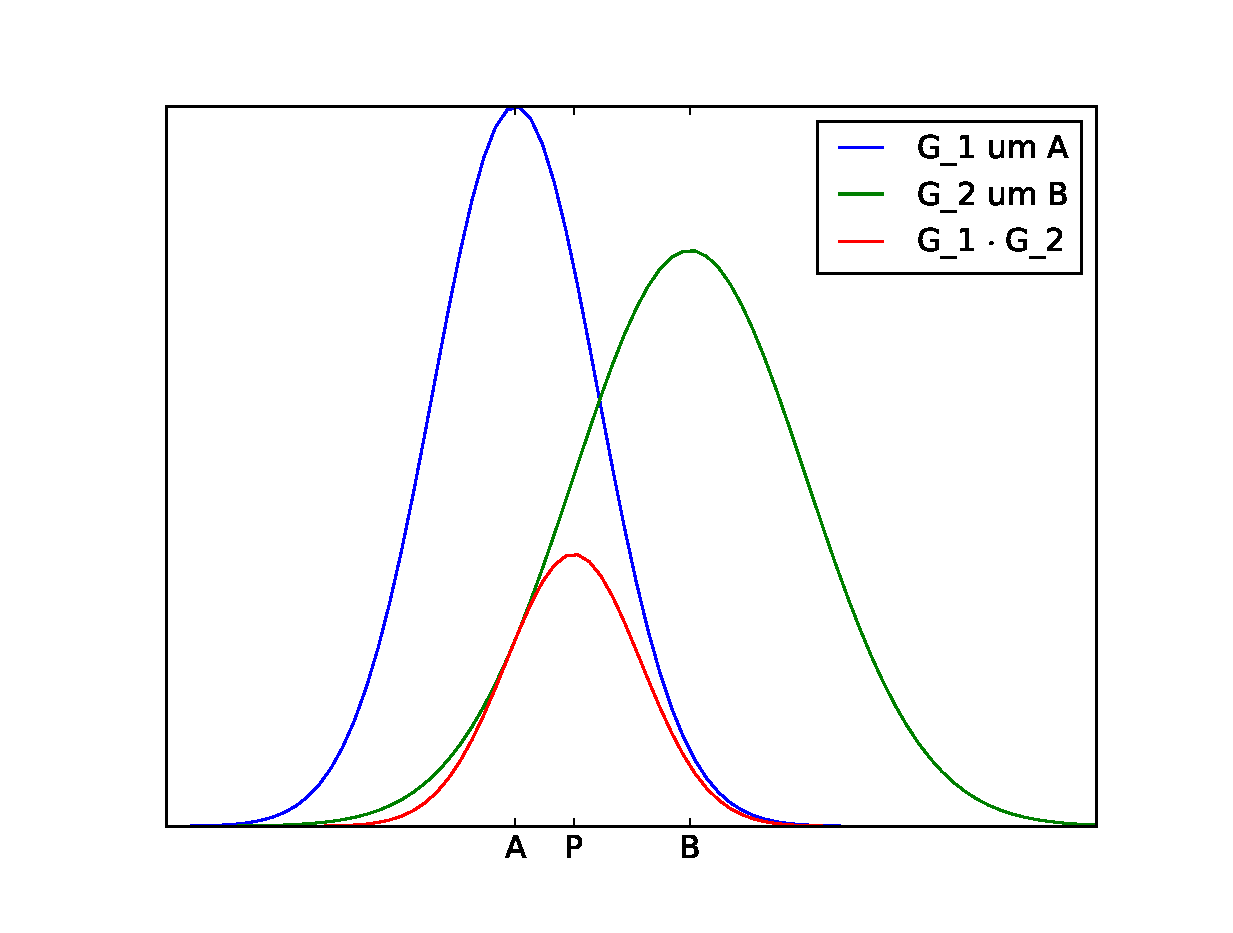
\includegraphics[scale=0.6]{GF.eps}
%	\vspace*{-7mm}
%	\caption{Eindimensionales Beispiel für das Produkt zweier beliebiger 
%	Gauß-Funktionen (vgl. \ref{eq:Produktansatz}). Die Lage des neuen Maximas 
%	ergibt sich durch 
%	\ref{eq:neuesZentrum_P}.}
%	\label{pic:1d_GTO} 
%\end{figure}
%
Dieses Vorgehen lässt sich beliebig oft wiederholen, was ein 
besonderer Vorteil für die oben erwähnten 4-Zentrenintegrale darstellt. Das 
Produkt von zwei nicht normierten GTOs lässt sich in eine 
Summe
%
\begin{align}
\psi_a(\textbf{r}_1)\cdot \psi_b(\textbf{r}_1) &=  x_A^i\,y_A^k\,z_A^m\cdot  
x_B^j\,y_B^l\,z_B^n\cdot e^{-b r_B^2-a 
		r_A^2}\\
%
&= \sum_{t=0}^{i+j}E^{i,j}_t\ 
\sum_{u=0}^{k+l}E^{k,l}_u\ \sum_{v=0}^{m+n}E^{m,n}_v\ 
\Lambda_{tuv}(\textbf{r}_1,p,\textbf{P})
\end{align}
%
über
%
\begin{align}
\Lambda_{tuv}(\textbf{r}_1,p,\textbf{P})&=\frac{\text{d}^t}{\text{d}P_x^t}\frac{\text{d}^u}{\text{d}P_y^u}\frac{\text{d}^v}{\text{d}P_z^v}\
 \exp(-p r_{1,P}^2)
\end{align}
%
schreiben.
Die nötigen Koeffizienten werden 
rekursiv mithilfe von
%
\begin{align}\label{eq:E:coef1}
E_0^{0,0}&=\exp(-\frac{ab}{p}(A_x-B_x)^2)\\\label{eq:E:coef2}
E_0^{i+1,j}&=-\frac{b}{p}(A_x-B_x)E^{i,j}_0 + E_1^{i,j}\\\label{eq:E:coef3}
E_0^{i,j+1}&=\frac{a}{p}(A_x-B_x)E^{i,j}_0 + E_1^{i,j}\\\label{eq:E:coef4}
E_t^{i,j} &= \frac{1}{2pt}\rl{iE^{i-1,j}_{t-1}+jE^{i,j-1}_{t-1} }
\end{align}
%
berechnet (siehe z.B. auch \cite{av:3a}), wobei das neue Zentrum durch
%
\begin{align}\label{eq:neuesZentrum_P}
p:=a+b \qquad, \qquad
\textbf{P}:=\frac{a\textbf{A}+b\textbf{B}}{p}
\end{align}
%
bestimmt ist. Eine analoge Umformung kann für das 
zweite Teilchen (\textbf{r}$_2$) mit
%
\begin{align}\label{eq:Q}
q:=c+d \qquad, \qquad
\textbf{Q}:=\frac{c\textbf{C}+d\textbf{D}}{q}
\end{align}
%
durchgeführt werden. Weiterhin zeigt Boys, dass alle Integrale dieses Typs eine 
%TODO ACHTUNG ZEILENTRENNUNG in finaler Version pruefen
|\textbf{P}-\textbf{Q}| Abhängigkeit haben, das heißt, dass sie nicht von den 
einzelnen Komponenten der Vektoren \textbf{P} und \textbf{Q} abhängen. Daher  
gilt 
%
$\rl{\frac{\DEL}{\DEL P_x}}^i = \rl{-\frac{\DEL}{\DEL 
Q_x}}^i=(-1)^i \rl{\frac{\DEL}{\DEL Q_x}}^i$
%
, was für das gesamt Integral bedeutet:
%
\begin{align}\label{eq:E:Koef}
I &= % N_{ikm}(a)N_{jln}(b)N_{i'k'm'}(c)N_{j'l'n'}(d) \cdot \\ 
%& \cdot 
\sum_{t=0}^{i+j}E^{i,j}_t\ \sum_{u=0}^{k+l}E^{k,l}_u\ 
\sum_{v=0}^{m+n}E^{m,n}_v\ (-1)^{t+u+v} \sum_{t'=0}^{i'+j'}E^{i',j'}_{t'}\ 
\sum_{u'=0}^{k'+l'}E^{k',l'}_{u'} \sum_{v'=0}^{m'+n'}E^{m',n'}_{v'}\ 
R^{t+t',u+u',v+v'}\ ,
\end{align}
%
wobei die gestrichenen Indizes für die Potenzen der GTO des 
zweiten Teilchens 
(\textbf{r}$_2$) stehen. Weiterhin wird die Schreibweise
% 
\begin{align}\label{eq:McM-D:kartesieAbleitungen}
R^{\tau,\rho,\sigma}&=\frac{d^\tau}{dQ^\tau_x}\ 
\frac{d^\rho}{dQ^\rho_y}\ \frac{d^\sigma}{dQ^\sigma_z}\ 
B\\\label{eq:basisint1}
B&= \int \int d\textbf{r}_1 d\textbf{r}_2 \ e^{-pr_{1,P}^2} \cdot 
f_{12}(r_{12}) \cdot e^{-qr_{2,Q}^2} \quad.
\end{align}
%
genutzt, wobei $B$ das sogenannte \textit{Basisintegral}  ist. Weiter wird dem 
McMurchie-Davidson Schema nicht gefolgt. 
%
%
%
\subsubsection{Analytische Modifikationen des Basisintegrals}\label{sec:modifik}
%
Als zweiten Schritt vereinfacht \cite{av:1a} das Basisintegral :
\begin{enumerate}
	\item[1.]  Es wird beobachtet, dass ,wie erwähnt, $B$ nur 
	von 
	|\textbf{P}-\textbf{Q}| abhängt. Daher kann nun eine 
	Koordinatenverschiebung 
	vorgenommen werden, sodass sich ein Punkt (z.B. \textbf{P}) im Ursprung 
	befindet\footnote{Im folgenden wird \textbf{Q}$_\text{neu}$ weiterhin mit 
	\textbf{Q} bezeichnet.}.\\
	$\Rightarrow \ \textbf{P}_\text{neu2}=0\ , \qquad 
	\textbf{Q}_{\text{neu}}=\textbf{Q}-\textbf{P}$
	%
	%
	\item[2.] Anschließend wird die noch verschobene Gauß-Funktion in 
	Kugelflächenfunktionen und modifizierte sphärische Besselfunktionen der 
	ersten Art entwickelt. Es gilt:
	\begin{align}
	e^{-qr_{2,Q}^2}=4\pi 
	e^{-qQ^2}\sum_{l=0}^{\infty}i_l(2qQr_2)\sum_{m=-l}^{+l} 
	Y_{lm}^*(\hat{Q})Y_{lm}(\hat{r}_2) \quad,
	\end{align}
	wobei $Q=|\textbf{Q}|$ ist. Diese Gleichung kann durch 
	die Verwendung von zum Beispiel \cite{b:5a} gezeigt 
	werden.
	Da über den gesamten Raum integriert wird, entfallen aus  
	Symmetriegründen 
	alle Terme außer l=0 ($\rightarrow$ m=0). Daher verbleibt B bei
	\begin{align}\label{eq:Basisintegral:zwerg}
	B=e^{-qQ^2} \int \int d\textbf{r}_1 d\textbf{r}_2\ e^{-pr_1^2-qr_2^2} 
	\frac{\sinh(2qQr_2)}{2qQr_2}\cdot f_{12}(r_{12}) \quad .
	\end{align}
	%
	%
	\item[3.] Als letzte Umformung wird eine Koordinatentransformation 
	durchgeführt. Hierbei geht man in ein System, indem ein Teilchen  im 
	Ursprung und das zweite auf der z-Achse liegt. Anschließend geht man in 
	Kugelkoordinaten. Die daraus resultierende Integralbildung wird z.B. in 
	\cite{av:6a} beschrieben. 
	%
	\begin{align*}
	\{x_1,y_1,z_1,x_2,y_2,z_2\}\rightarrow\{r_1,r_2,r_{12},\alpha,\beta,\gamma\}
	\end{align*}
	%
	
	$\alpha,\beta$ und $\gamma$ sind resultierende Eulerwinkel, die entstehen, 
	wenn das Koordinatensystem 1 (\textbf{r}$_1$) derart 
	gedreht wird, dass 
	der Vektor \textbf{r}$_2$ auf der z-Achse liegt. 
	Weiterhin muss erwähnt werden, dass offensichtlich d\textbf{r}$_1$ = 
	d\textbf{r}$_{12}$ gilt, wodurch sich im Gegensatz zu \cite{av:6a} die 
	Bedeutung von $r_1$ und	$r_{12}$ vertauscht. 
	Da außerdem $r_1=|\textbf{r}_{12}+\textbf{r}_2|$ gilt, 
	folgt nach elementarer Winkelintegration für allgemeine Funktionen f,g und 
	h:
	\footnote{$\textbf{r}_1=\textbf{r}_{12}+\textbf{r}_{2},\ 
		r_1=\sqrt{r_{12}^2+r_2^2-2r_{12}r_2\cos(\beta)},\ 
		d\textbf{r}_{12}= r^2_{12} \sin(\beta) \ dr_{12}\ d\alpha\ d\beta$} 
%
	\begin{align}\nonumber
		\int \int & f(r_{1}) g(r_2)h(r_{12}) d\textbf{r}_1d\textbf{r}_2 =\\
		% 
		& 8\pi^2\int_{0}^{\infty}h(r_{12})\ r_{12}\ dr_{12}\int_{0}^{\infty} 
		g(r_2)\ r_2\ dr_2 \int_{|r_{12}-r_2|}^{r_{12}+r_2}f(r_{1})\ r_{1}\ 
		dr_{1}\quad.
	\end{align}
	Nach Integration (vergleiche \ref{eq:Basisintegral:zwerg} ) über $r_1$ und 
	$r_2$ verbleibt
	\begin{align}\label{eq:B:zwischenErg}
		B= \sqrt{\frac{\pi^5}{p+q}}\frac{1}{pq}\cdot \int_{0}^{\infty}dr_{12}\ 
		f_{12}(r_{12})\cdot r_{12}\cdot \rl{\frac{e^{-  
		\frac{pq}{p+q}(r_{12}-Q)^2}-e^{-\frac{pq}{p+q}(r_{12}+Q)^2}}{Q}}\quad .
	\end{align}
\end{enumerate} 
%
Im Folgenden wird die zusammenfassende Größe
%
\begin{align}
\xi := \frac{p\cdot q}{p+q}
\end{align}
%
verwendet, um \ref{eq:B:zwischenErg} zu vereinfachen.
%
%
%
\subsubsection{Hobson Theorem und 
Schlegel-Koeffizienten}\label{sec:Hobson_schlegel}
%
Wie in \ref{eq:McM-D:kartesieAbleitungen} zu erkennen ist, müssen  
Ableitungen des Basisintegrals berechnet werden\footnote{In der Arbeit 
\cite{av:9a} ist eine genauere und z.T. berichtigte Version dieses Teils des 
Algorithmus aus \cite{av:1a} beschrieben.}. Da B nur von $Q=|Q|$ abhängt, 
ist es sinnvoll, die kartesischen Ableitungen in sphärische Ableitungen nach 
$Q$ umzuformen.\\
Dazu wird als Erstes auf die Arbeit \cite{av:4a} verwiesen, in der ein 
vollständiger, analytischer Ausdruck für die Umformung von sphärische in  
kartesische GTOs (Koordinatenwechsel des polynomartigen Anteils) präsentiert 
wird. Die Rückumformung, das heißt die Umformung von kartesischen in 
sphärische Koordinaten, kann nach Absprache mit den Autoren von \cite{av:1a} 
wie folgt dargestellt werden. Sind $c_{l_xl_yl_z}^{l,m}$ die reellen 
Schlegel-Koeffizienten aus \cite{av:4a}, so können die Koeffizienten der 
Rückumformung mit
%
\begin{align}\nonumber
c^{-1}(l,m,l_x,l_y,l_z)&=\frac{2}{\Gamma\rl{\frac{l_x+l_y+l_z+l+3}{2}}} 
 \ \cdot \\ \label{eq:def:c_koef}
 &\cdot  \sum_{a+b+c\leq l} c_{l_xl_yl_z}^{lm}\cdot 
\Gamma\rl{\frac{1+l_x+a}{2}}\cdot 
\Gamma\rl{\frac{1+l_y+b}{2}}\cdot \Gamma\rl{\frac{1+l_z+c}{2}}
\end{align}
%
berechnet werden. Damit ist also die Umformung
%
\begin{align}\label{eq:trafo_c-1}
x^{l_x}y^{l_y}z^{l_z} = \sum_{l=0}^{l_{max}}\sum_{m=0}^l 
c^{-1}(l,m,l_x,l_y,l_z)\cdot r^{l_{max}-l} Z_{lm}(\textbf{r})
\end{align}
%
möglich. $Z_{lm}(\textbf{r})=r^l\cdot Y_{lm}(\hat{\textbf{r}})$ sind die 
reellen, soliden 
Kugelflächenfunktionen ohne Racah's Normalisierung und 
$l_{max}=l_x+l_y+l_z$. Eine detailliertere Beschreibung inkl. aller 
Definitionen bzgl. dieser Transformation ist im Anhang 
\ref{sec:AnhangA:Schlegel} zu finden. Weiterhin sei erwähnt, 
dass auch 
\cite{av:4a} einige kleinere Tippfehler hat, welche in Anhang berichtigt sind.\\

Analog dazu können mithilfe der selben Koeffizienten auch die 
Differenzialoperatoren \ref{eq:McM-D:kartesieAbleitungen} umgeformt werden. 
Mit der Verwendung des Hobson Theorems in der Form
%
\begin{align}\label{eq:Hobson}
\Op{Z}_{lm}(\nabla_Q)g(Q)=\left[\mathcal{D}^l_Qg(Q)\right]Z_{lm}(\textbf{Q}) 
\end{align}
%
können die kartesischen Ableitungen durch 
%
\begin{align}
R^{\tau,\rho,\sigma}=\frac{d^\tau}{dQ^\tau_x}\ 
\frac{d^\rho}{dQ^\rho_y}\ \frac{d^\sigma}{dQ^\sigma_z}\ 
B=\sum_{l=0}^{l_{max}}\sum_{m=-l}^{l}c^{-1}(l,m,\tau,\rho,\sigma)\cdot
 \nabla_Q^{l_{max}-l}\left[(\mathcal{D}_Q^lB)Z_{lm}(\textbf{Q})\right]
\end{align}
%
ausgedrückt werden, wobei $\mathcal{D}^l_Q=Q^{-1}\DEL_Q$ darstellt. Ist  
$l_{max}-l$ 
ungerade, so ist $c^{-1}=0$. Mithilfe der Relation 
$\nabla_Q^2=Q^2\mathcal{D}^l_Q+3\mathcal{D}_Q$ 
kann nun \ref{eq:McM-D:kartesieAbleitungen} in die finale Form
%
\begin{align}\label{eq:final:Hobson}
R^{\tau,\rho,\sigma}=\sum_{l=0}^{l_{max}}\sum_{m=-l}^{l}c^{-1}(l,m,\tau,\rho,\sigma)Z_{lm}(\textbf{Q})
 \sum_{k=0}^{k_{max}}d_k^{l,k_{max}} \cdot 
\left[(\mathcal{D}_Q^{l_{max}-k}B)\right]Q^{l_{max}-l-2k}
\end{align}
%
geschrieben werden. Hierbei ist $k_{max}=\frac{1}{2}(l_{max}-l)$ und die 
Koeffizienten $d_k^{l,k_{max}}$ können rekursiv berechnet werden:
%
\begin{align}\nonumber
d_n^{l,m}=d_n^{l,m-1} &+\left[2l+3+4(m-n)\right]d_{n-1}^{l,m-1}+\\ 
\label{eq:rek_d}
&2(m-n+1)(2l+3+2(m-n))d_{n-2}^{l,m-1} \qquad.
\end{align} 
%
Die Rekursion startet bei $d_{-1}^{l,m}=0$ und $d_0^{l,m}=1$.
%
%
%
\subsubsection{Radiale Ableitungen der Basisintegrale}
%
Der letzte in der Arbeit \cite{av:1a} präsentierte Schritt 
sieht die 
Evaluation der radialen Ableitungen des Basisintegrals vor. Dazu werden zwei 
Vorgehensweisen dargestellt. Die erste in der vorliegenden 
Arbeit nicht 
behandelte Vorgehensweise nutzt eine Taylorentwicklung\footnote{In den Formeln 
(44)-(46) von \cite{av:1a} ist bei der Umformung der Exponentialfunktionen in 
den sinh ein Faktor 2 verlorengegangen. Weiterhin fehlt im 
ersten Term von 
(47) ein weiterer Faktor 2.} von $Q$ um 0 aus. Da im Regime der ultrakalten 
Gase der Bereich von sehr kleinen Teilchenabständen ($Q$) eher uninteressant 
ist\footnote{Da in diesem Bereich die harmonische Falle vernachlässigt werden 
kann und die Schrödingergleichung in Relativ- und Schwerpunktkoordinaten 
separiert und somit in 1D lösbar ist.}, wird nun das zweite Vorgehen für 
mittlere und große $Q$ erläutert.\\

Das Basisintegral \ref{eq:Basisintegral:zwerg} kann in zwei Terme 
geschrieben werden. Mithilfe der Definition 
%
\begin{align}
\mathcal{H}^\pm_{jkl}&:=\sqrt{\frac{\pi^5}{p+q}}\frac{1}{pq} \int_{0}^{\infty} 
dr_{12}\ r_{12}^j\ \cdot 
\rl{\frac{1}{Q}\frac{\text{d}}{\text{d}Q}}^l\rl{\frac{e^{-\xi(r_{12}\pm 
			Q)^2}}{Q^k}}
\end{align}
%
gilt
%
\begin{align}\label{eq:diff_op}
\mathcal{D}_Q^lB=\left[\rl{\frac{1}{Q}\frac{d}{dQ}}^lB\right] 
=\rl{\mathcal{H}^-_{11l}-\mathcal{H}^+_{11l}} \quad .
\end{align}
%
Durch abermalige Anwendung des Differentialoperators $\mathcal{D}_Q$ kann die 
Rekursion
%
\begin{align}\label{eq:rek:H}
\mathcal{H}_{jkl}^{\pm} = \mp 2\xi\cdot \mathcal{H}_{j+1,k+1,l-1}^\pm-2\xi\cdot 
\mathcal{H}_{j,k,l-1}^\pm-k\cdot\mathcal{H}_{j,k+2,l-1}^\pm
\end{align}
%
gefunden werden. Man beobachtet, dass auf Kosten von j und k der Index l für 
die Ableitungen reduziert werden kann. Durch die trivialen Relationen
\begin{align} \label{eq:prop:H}
\mathcal{H}_{jk0}^{\pm} &= \frac{1}{Q^k} \cdot \mathcal{H}_{j00}^\pm\\ 
\mathcal{H}_{j00}^{\pm} &=\sqrt{\frac{\pi^5}{p+q}}\frac{1}{pq} \cdot \Pi_j^\pm
\end{align}
vereinfacht sich das nun noch zu berechnende Integral auf
\begin{align}\label{eq:PI-Integrale}
\Pi_j^\pm= \int_{0}^{\infty}dr_{12}\ r_{12}^j \cdot f_{12}(r_{12}) \cdot 
e^{-\xi (r_{12} \pm Q)^2}\quad .
\end{align}
%
%
%
\subsubsection{Zusammenfassung}\label{sec:Zusammenfassung:Algorithmus}
%
Ziel des Algorithmus ist es gewesen, 
%
\begin{align}\nonumber
I= \int \int\ 
d\textbf{r}_1\ d\textbf{r}_1 
(\psi_i^a(\textbf{r}_1)\psi_i^c(\textbf{r}_2))^* f_{12}(r_{12}) 
\psi_j^b(\textbf{r}_1)\psi_j^d(\textbf{r}_2)
\end{align}
%
zu berechnen. Mithilfe des Ansatzes der GTOs kann die Integralberechnung   
auf die Schar der $\Pi_j^\pm$ Integrale \ref{eq:PI-Integrale}
%
\begin{align}\nonumber
\Pi_j^\pm= \int_{0}^{\infty}dr_{12}\ r_{12}^j \cdot f_{12}(r_{12}) \cdot 
e^{-\xi (r_{12} \pm Q)^2}
\end{align}
% 
zurückgeführt werden. Wichtig hierbei ist die korrekte Definition von $Q$ 
(\ref{eq:Q}) mit Berücksichtigung der Koordinatenverschiebung in 
\ref{sec:modifik}, bei der P auf den Ursprung verschoben 
wird. Anschließend 
ermittelt man mithilfe der Rekursion \ref{eq:rek:H}
%
\begin{align}\nonumber
\mathcal{H}_{jkl}^{\pm} = \mp 2\xi\cdot \mathcal{H}_{j+1,k+1,l-1}^\pm-2\xi\cdot 
\mathcal{H}_{j,k,l-1}^\pm-k\cdot\mathcal{H}_{j,k+2,l-1}^\pm
\end{align}
%
und den benötigten Proportionalitäten \ref{eq:prop:H} die Integrale 
$\mathcal{H}_{11l}^\pm$. \\
Via \ref{eq:final:Hobson} mit \ref{eq:diff_op}
%
\begin{align}\label{R_sum}
R^{\tau,\rho,\sigma}=\sum_{l=0}^{l_{max}}\sum_{m=-l}^{l}c^{-1}(l,m,\tau,\rho,\sigma)Z_{lm}(\textbf{Q})
\sum_{k=0}^{k_{max}}d_k^{l,k_{max}} \cdot 
\left[(\mathcal{H}^-_{11l}-\mathcal{H}^+_{11l})\right]Q^{l_{max}-l-2k}
\end{align}
%
und \ref{eq:E:Koef} 
%
\begin{align}\nonumber 
I &= %N_{ikm}(a)N_{jln}(b)N_{i'k'm'}(c)N_{j'l'n'}(d) \cdot \\ \nonumber
%& \cdot 
\sum_{t=0}^{i+j}E^{i,j}_t\ \sum_{u=0}^{k+l}E^{k,l}_u\ 
\sum_{v=0}^{m+n}E^{m,n}_v\ (-1)^{t+u+v} \sum_{t'=0}^{i'+j'}E^{i',j'}_{t'}\ 
\sum_{u'=0}^{k'+l'}E^{k',l'}_{u'} \sum_{v'=0}^{m'+n'}E^{m',n'}_{v'}\ 
R^{t+t',u+u',v+v'}
\end{align}
%
ist das Integral berechnet. \\

Dieses Vorgehen ist unabhängig von der Form der eingesetzten Funktion 
$f_{12}(r_{12})$, solange die Abhängigkeit $r_{12}=|\textbf{r}_1-\textbf{r}_2|$ 
stimmt. $\Pi^\pm_j$ kann sowohl analytisch als auch im Allgemeinen numerisch 
gelöst werden. Auf mögliche Probleme dabei wird im folgenden Abschnitt 
eingegangen. Die Normierungskonstanten $N$ können ohne Beschränkung der 
Allgemeinheit auch weggelassen werden. Dies entspricht der Verwendung von 
nicht normierten GTOs als Basisfunktionen.
%
%
%
\subsection{Berechnung der Basisintegrale}
%
Dieser Abschnitt widmet sich der Betrachtung der $\Pi_j^\pm$-Integrale. Im 
Regime der ultrakalten Gase und unter der Verwendung des Hamiltonoperators 
\ref{eq:kernHam1} ist leicht zu sehen, dass die Funktion $f_{12}$ die 
Ortsdarstellung des Wechselwirkungsoperators 
($\hat{=}$Wechselwirkungspotential) 
$\Op{U}(r_{12})$ darstellt. Alle restlichen Operatoren 
bedürfen keiner 
Zweiteilchenintegralen. Prinzipiell ist der Algorithmus auch für 
Einteilchenintegrale benutzbar, jedoch soll vorher geprüft 
werden, ob andere 
existierende Einteilchenintegral-Algorithmen nicht effektiver 
sind\footnote{Außerdem muss die Implementierung im Kapitel 
\ref{sec:Implementierung} entsprechend angepasst werden.}.\\
Für das oben beschriebene System ist kein analytisches 
Wechselwirkungspotential bekannt. Aus numerischen Elektronenstrukturrechnungen 
und Experimenten kann jedoch ein numerisches Potential angegeben werden 
\cite{phdthesis:sergey}. Ein Problem im Regime der 
ultrakalten Gase ist,  dass Wechselwirkungspotentiale eine 
Divergenz im Ursprung haben. Diese entstehen aus dem Fakt, dass zwei Atome 
nicht am exakt selben Ort sein können. Die Wellenfunktion muss aus 
physikalischer Sicht dort exakt Null sein und im Bereich des starken Anstiegs 
des Potentials exponentiell abfallen. Die GTOs erfüllen diese Randbedingungen 
im Allgemeinen nicht. Daher ist die prinzipielle Divergenz in $\Pi^\pm_j$ nicht 
überraschend. Eine rein numerische Funktion $f_{12}$ mit Divergenz in 0 ist 
damit für das Integral nur schwer anwendbar. Die 
Basisfunktionen müssen so 
gewählt werden, dass die Divergenz nicht zum Tragen kommt, 
das heißt, dass der 
"Flächeninhalt"\ direkt um 0 zu vernachlässigen ist. Die 
Basisfunktionen müssen 
dort also im Rahmen der Numerik verschwinden.\\%TODO vlt ein Bild zeigen 
%beidem ein   %solcher Fall gezeigt ist.
Weiterhin kann versucht werden, die numerische Integration zu 
renormieren, indem 
zum Beispiel nicht bis exakt 0, sondern zu einem speziellen Wert $\epsilon>0$  
integriert wird. Das Problem hierbei ist, $\epsilon$ so zu bestimmen, dass das 
Integral noch alle benötigten Informationen enthält und so ein physikalisch 
sinnvolles Ergebnis entsteht. Da dieses Vorgehen eher ungenau und $\epsilon$ 
numerisch noch nicht motiviert ist, wird dieses Vorgehen hier nicht weiter 
verfolgt.\\
Ein dritter Weg stellt eine analytische Funktion für $f_{12}$ dar, das heißt 
eine durch Parameter optimierte Näherungsfunktion für das numerische Potential 
(ein Fit ). Zwei bekannte Näherungsfunktionen für ein numerisches 
Wechselwirkungspotential zwischen Atomen stellen das 
Lennard-Jones- (kurz LJP) 
und das Morse-Potential (kurz MRP) dar. Beide haben qualitativ
einen ähnlichen Verlauf und sind in der Quantenchemie gebräuchlich.\\
Vorteil des Lennard-Jones-Potentials ist das korrekte asymptotische Verhalten 
für große Abstände mit $\sim -\frac{C}{r^6}$, wobei C ein 
Van-der-Waals-Koeffizient darstellt. Dagegen hat das Morse-Potential eine etwas 
einfachere mathematische Form. Beide können durch Angabe der erwarteten 
(gemessenen) Dissoziationsenergie und der Lage des Minimums 
bestimmt 
werden. Das Morse-Potential hat außerdem einen weiteren 
Parameter, den 
Exponenten, der die Steilheit bzw. auch Steifheit genannt, 
der Kurve 
manipuliert.\\

Im Folgenden werden beide hier erwähnten Potentiale erklärt und im Rahmen des 
$\Pi^\pm_j$ Integrals diskutiert und berechnet.
%
%
%
\subsubsection{Wechselwirkungspotentiale:}
\subparagraph{Das Morse-Potential} hat die drei Schreibweisen  
%
\begin{align}\label{eq:MRP}
V_{\text{MRP}}(r_{12}) &= D_e\cdot \rl{1-e^{-a_\text{st}\cdot(r_{12}-R_m)}}^2 
-D_e\\
                       &= D_e\cdot 
                       \rl{e^{-2a_\text{st}(r_{12}-R_m)}-2e^{-a_\text{st}(r_{12}-R_m)}}\\
                       &=A_{\text{MRP}}\cdot e^{-2a_\text{st} r_{12}} + 
                       B_{\text{MRP}}\cdot e^{-a_\text{st} r_{12}} \quad,
\end{align}
%
wobei $D_e$ die Dissoziationsenergie , $R_m$ die Lage des Minimums und $a$ ein 
an sich beliebiger positiver reeller Parameter ist.  Die Koeffizienten 
$A_\text{MRP} \text{ und  }B_\text{MRP}$ können als Zusammenfassung vieler 
Parameter 
aufgefasst werden, um die numerische Behandlung zu vereinfachen. \\
Das folgende Bild (\ref{pic:MRP_1}) veranschaulicht das Morse-Potential und die 
Abhängigkeit 
bzgl. des Exponenten.
%
%\begin{figure}[H] \centering
%	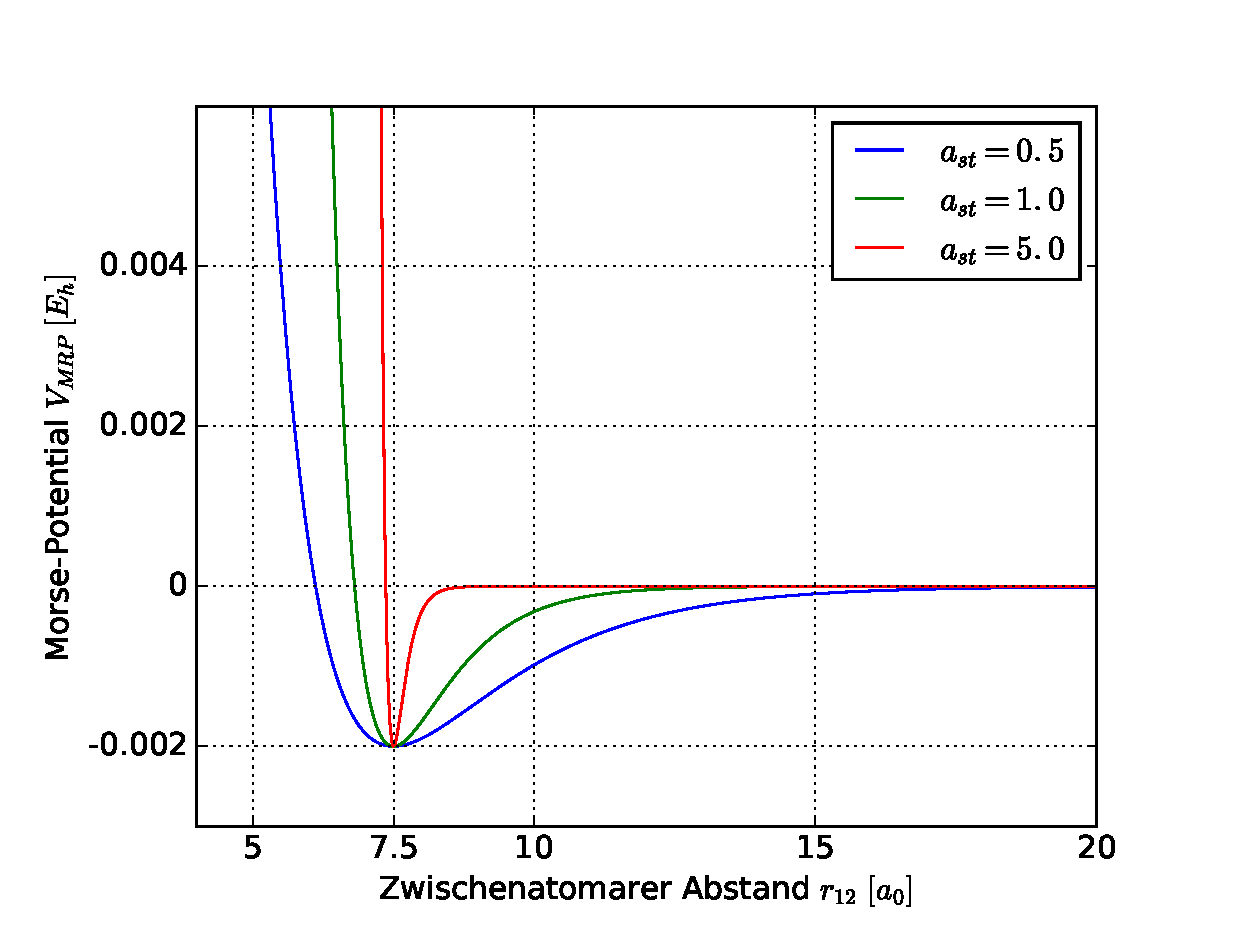
\includegraphics[scale=0.65]{MRP.eps}
%%	\vspace*{-10mm}
%	\caption{Es ist das Morse-Potential \ref{eq:MRP} mit fixierten Parametern 
%	$D_e = 0.002\ E_h$ und $R_m = 7.5\ a_0$ zu verschiedenen Exponenten 
%	$a_\text{st}$ im 
%	Bereich von 0.5 bis 5.0 dargestellt.}%TODO anderes Bild / vorallem andere 
%	%achsenbeschreiftungen !!!
%	\vspace{2mm} %\hrule 
%	\label{pic:MRP_1} 
%\end{figure}
%
Nun soll das Morsepotential als Funktion $f_{12}$ in das $\Pi^\pm_j$ - 
Integral  \ref{eq:PI-Integrale} eingesetzt werden:
%
\begin{align}
\Pi_j^\pm & =\int_{0}^{\infty}dr_{12}\ r_{12}^j \cdot V_\text{MRP}(r_{12}) \cdot
           e^{-\xi (r_{12} \pm Q)^2}\\
          & = \int_{0}^{\infty}dr_{12}\ r_{12}^j \cdot \rl{A_{\text{MRP}}\cdot 
          e^{-a_\text{st} r_{12}} + B_{\text{MRP}}\cdot e^{-2a_\text{st} 
          r_{12}}} \cdot e^{-\xi 
          (r_{12} \pm Q)^2} \\ \label{eq:PI_MRP}
          & = A^\prime_{\text{MRP}}\cdot \int_{0}^{\infty}dr_{12}\ r_{12}^j 
          \cdot e^{b_1\cdot r_{12} - \xi r_{12}^2} + B^\prime_\text{MRP}\cdot 
          \int_{0}^{\infty}dr_{12}\ r_{12}^j \cdot e^{b_2\cdot r_{12} - \xi 
          r_{12}^2}
\end{align}
%
Hierbei sind die Parameter $A^\prime_\text{MRP},\ B^\prime_\text{MRP},\ b_1$ 
und $b_2$ Zusammenfassungen von Konstanten. Diese sind durch
%
\begin{align}
A^\prime_\text{MRP}&:=A_\text{MRP}\cdot e^{-\xi Q^2}= D_e\cdot 
e^{2a_\text{st}R_m} \cdot 
e^{-\xi Q^2}\\
B^\prime_\text{MRP}&:=B_\text{MRP}\cdot e^{-\xi Q^2}= -2\cdot D_e\cdot 
e^{a_\text{st}R_m} 
\cdot e^{-\xi Q^2}\\
b_1 &:=-(a_\text{st}\pm 2\xi Q)\\
b_2 &:=-2(a_\text{st} \pm \xi Q )
\end{align}
%
definiert. Wie man an \ref{eq:PI_MRP} erkennt, kann das $\Pi^\pm_j$-Integral 
durch ein verallgemeinertes Integral über ein Monom des Grades j und einer 
Exponentialfunktion berechnet werden. Die Evaluation des Integraltyps
%
\begin{align}\label{eq:def:S}
S(\alpha,\beta,\gamma):=\int_{0}^{\infty}\ dx\ x^\alpha\cdot e^{\beta x - 
\gamma 
x^2}
\end{align}
%
wird im Abschnitt III.B-C der Arbeit \cite{av:1a} diskutiert. Für 
$\alpha\geq-1$, $\alpha\in \mathbb{N}, (\beta,\gamma)\in\mathbb{R}$ und $\gamma 
>0$  kann das Integral 
regulär berechnet werden. Für das MRP sind diese Forderungen immer 
erfüllt\footnote{da $\alpha=j$ wobei $j\in \mathbb{N}$ und $j\geq1$ mit 
$\beta=\{b_1,b_2\}$ und $\gamma=\xi$}, sodass das Integral ohne 
weitere Näherungen berechnet werden kann. $\Pi_j^\pm$ lässt sich damit 
also 
durch
%
\begin{align}\label{eq:PIinS_MRP}
\Pi^\pm_j=A^\prime_\text{MRP}\cdot 
S(j,b_1,\xi)+B^\prime_\text{MRP}\cdot 
S(j,b_2,\xi)
\end{align}
%
ausdrücken. In dieser Arbeit wird S mithilfe von 
%
\begin{align}\nonumber
S(\alpha,\beta,\gamma)  
&=(2\sqrt{\gamma})^{-\alpha-1}\Gamma(\alpha+1)\sqrt{\pi}\cdot
\left[\frac{M\rl{\frac{\alpha+1}{2},\frac{1}{2},\frac{\beta^2}{4\gamma}}}{\Gamma(\alpha/2+1)}
+\frac{\beta}{\sqrt{\gamma}} 
\frac{M\rl{\frac{\alpha}{2}+1,\frac{3}{2},\frac{\beta^2}{4\gamma}}}{\Gamma((\alpha+1)/2)}\right]\\\nonumber
%
&=\frac{1}{2}\, \gamma^{-1 - \frac{\alpha}{2}}\cdot \bigg[\beta\cdot 
\Gamma\rl{1 + \frac{\alpha}{2}}M\rl{1 + \frac{\alpha}{2}, \frac{3}{2}, 
\frac{\beta^2}{4\gamma}} \\ \label{eq:S,alpha>0}
&\qquad \qquad \qquad +\sqrt{\gamma}\cdot \Gamma\rl{\frac{1+\alpha}{2}}\cdot 
M\rl{\frac{1 + 
\alpha}{2}, 
\frac{1}{2},\frac{\beta^2}{4\gamma}} \bigg]
\end{align}
%
berechnet, wobei M Krummers konfluierte hypergeometrische Funktion ( auch mit 
$_1F_1$ bezeichnet) darstellt. Diese wird wiederum durch die 
Reihendarstellung 
%
\begin{align}\label{eq:reihe_M_kon.hyp.geo}
M(a,b,z)=1+\frac{az}{b}+\frac{(a)_2z^2}{(b)_2 
2!}+\dots +\frac{(a)_nz^n}{(b)_nn!}+\dots
\end{align}
mit den Pochhammer-Symbol
\begin{align}
(a)_n=a(a+1)(a+2)\dots(a+n-1), \ (a)_0=1
\end{align}
% 
berechnet (vergleiche mit \cite{b:1a} und \cite{b:6a}).\\
Erwähnt werden muss an dieser Stelle, dass \cite{av:1a} eine leicht andere 
Formel verwendet wird. In dieser Stelle findet Tricomis 
konfluierte 
hypergeometische Funktion 
($\mathcal{U}$) ihre Anwendung. Jedoch kann mit den im 
Vorfeld benutzten 
Konversionen  ( Definition (57) = Formel \ref{eq:def:S} ) die entsprechende 
Gleichung (60) aus \cite{av:1a} nicht abgeleitet werden\footnote{Es 
konnte 
sogar mithilfe eines kleinen MATHEMATICA-Skrips gezeigt werden, dass 
die linke 
Seite nicht der rechten entspricht. Durch Änderung der Definition 
\ref{eq:def:S} ($\beta\rightarrow-\beta$) und Vergleich mit 
\cite{b:6a} kann 
eine beinahe Übereinstimmung gefunden werden, jedoch müsste 
diese noch 
genauer 
geprüft und alle darauf folgenden Gleichungen in \cite{av:1a} 
angepasst werden. 
In dieser Arbeit wird diese Korrektur nicht weiter 
verfolgt.}. 
Dementsprechend wird 
auch nicht, der im unterstützenden Material \cite{av:1a2} 
dargestellte 
Weg zur Berechnung von $\mathcal{U}$ verwendet. Dieser berechnet $\mathcal{U}$ 
in verschiedenen Intervallen mit jeweils anderen Formeln, um die Konvergenz und 
Genauigkeit zu verbessern. Daher ist zu erwarten, dass auch 
\ref{eq:S,alpha>0} nicht für alle Bereiche der Parameter numerisch stabile 
Ergebnisse liefert\footnote{Es wird auch eine Integration 
durch quadratische 
Ergänzung des Exponenten und anschließender Umformung auf eine Erf-Funktion 
bzw. unvollständige $\Gamma$-Funktion 
versucht. Jedoch liefert dieses Vorgehen eine zu ungenaue 
Berechnung, da bei 
der auftretenden Subtraktion $1-\text{Erf}(x)$ schnell 
signifikante Stellen verloren gehen.}. Getestet wird diese Erwartung in Kapitel 
\ref{sec:Implementierung}. % (??) 
%
%
%
\subparagraph{Das Lennard-Jones-Potential} hat vor allem zwei gängige 
Darstellungen. Es muss erwähnt werden, dass in dieser Arbeit das sogenannte 
(12,6)-LJP benutzt wird:
%
\begin{align}\label{eq:def:LJP}
V_{\text{LJP}}(r_{12})&=D_e\cdot\left[ \rl{\frac{R_m}{r_{12}}}^{12} - 
2\rl{\frac{R_m}{r_{12}}}^6 \right]\\
                      &= 
                      \frac{A_\text{LJP}}{r_{12}^{12}}+\frac{B_\text{LJP}}{r^6_{12}}
                       \quad.
\end{align}
$D_e$ und $R_m$ sind analog zum MRP definiert. Auch $A_\text{LJP}$ und 
$B_\text{LJP}$ sind Zusammenfassungen von Konstanten:
%
\begin{align}
A_\text{LJP} &= D_e\cdot R_m^{12} \\
B_\text{LJP} &= -2\cdot D_e \cdot R_m^6 
\end{align}
%
Die Potenzen 12 bzw. 6 entstehen durch die betrachtete Wechselwirkung und 
Eigenschaften der Teilchen. Für neutrale, homonukleare Atome entsteht die 
Van-der-Waals Anziehung, die gut durch eine inverse sechste 
Potenz beschrieben 
werden kann. Der hier verwendete abstoßende Term mit der 
zwölften Potenz ist die
Konversion und kann im Zweifelsfall noch variiert werden. Im Gegensatz zum MRP 
hat das LJP in dieser Form keinen weiteren freien Parameter.\\
Für das $\Pi^\pm_j$-Integral ergibt sich:
%
\begin{align}
\Pi_j^\pm & =\int_{0}^{\infty}dr_{12}\ r_{12}^j \cdot V_\text{LJP}(r_{12}) \cdot
             e^{-\xi (r_{12} \pm Q)^2}\\\nonumber
          & = \int_{0}^{\infty}dr_{12}\ r_{12}^j \cdot 
          \rl{\frac{A_\text{LJP}}{r_{12}^{12}}+\frac{B_\text{LJP}}{r^6}}\cdot
          e^{-\xi (r_{12} \pm Q)^2}\\\nonumber
%\end{align}
%\begin{align}
%\Pi_j^\pm 
& = A^\prime_\text{LJP}\int_{0}^{\infty}dr_{12}\ r_{12}^j \cdot 
\frac{1}{r_{12}^{12}}\cdot e^{\mp 2\xi Q r_{12} -\xi r_{12}^2}+ 
B^\prime_\text{LJP}\int_{0}^{\infty}dr_{12}\ r_{12}^j 
\cdot\frac{1}{r_{12}^6}\cdot e^{\mp 2\xi Q r_{12} -\xi 
r_{12}^2}\\\nonumber
&=A^\prime_\text{LJP}\int_{0}^{\infty}dr_{12}\ r_{12}^{j-12}\cdot e^{\mp 2\xi Q 
r_{12} -\xi r_{12}^2}+ 
B^\prime_\text{LJP}\int_{0}^{\infty}dr_{12}\ r_{12}^{j-6}\cdot e^{\mp 2\xi Q 
r_{12} -\xi r_{12}^2}\\\label{eq:PI_LJP}
&=A^\prime_\text{LJP}\cdot 
S(\alpha_1,\beta,\gamma)+B^\prime_\text{LJP}\cdot 
S(\alpha_2,\beta,\gamma)\ .
\end{align}
%
Es ist zu erkennen, dass auch mit dem LJP  sich das $\Pi^\pm_j$-Integral auf 
den Typ \ref{eq:def:S} vereinfachen lässt. In diesem Fall gelten die 
Definitionen 
%
\begin{align}\nonumber
A^\prime_\text{LJP}:=A_\text{LJP}\cdot e^{-\xi Q^2} &\quad,\quad 
B^\prime_\text{LJP}:=B_\text{LJP}\cdot e^{-\xi Q^2} \\\nonumber
\alpha_1:=j-12 &\quad,\quad \alpha_2:=j-6 \\\nonumber
\beta&=\mp 2\xi Q\\
\gamma &= \xi \qquad,
\end{align}
wobei jedoch nun $\alpha$ auch eine negative ganze Zahl sein kann, da 
$j\geq1$ ist.  Die Integrale mit positiven $\alpha$ können analog zu 
\ref{eq:S,alpha>0} berechnet werden. Dagegen können die Integrale mit 
negativem $\alpha$ nicht regulär bestimmt werden. Sie sind divergent, da der 
Integrand einen Pol in 0 besitzt. Wie oben schon einmal erwähnt, ist eine 
Divergenz in 0 nicht überraschend, da die Gauß-Funktionen die Randbedingung in 
0 nicht erfüllen. Physikalisch gesehen ist jedoch eine Divergenz nicht 
realistisch (es könnte auch eine divergente Energie folgen). 
Dementsprechend kann eine Renormierung versucht werden. \cite{av:1a} schlägt in 
Abschnitt III.A. bzw. III.C. ein Renormierungsschema vor.\\
Hier zeigt sich eine entscheidende Schwäche des LJP als Näherungsfunktion. 
%
%
%
\subparagraph{Das Renormierungsschema} \label{sec:renorm}
%
soll auf Integrale des Typs 
%
\begin{align}\label{eq:def:T-Int}
T_s^\pm(x)&:=\mathcal{R}\int_{0}^{\infty}\frac{dz}{z^s}e^{\pm z-xz^2}
\end{align}
%
angewendet werden, welche dem besprochenen Fall von negativen 
$\alpha$ 
entsprechen. $\mathcal{R}$ steht dabei für die Anwendung einer 
Renormierung. 
Mit den Definitionen 
%
\begin{align}
s=-\alpha \qquad\text{und} \qquad x=\frac{\gamma}{\beta^2} 
\end{align} 
%
folgt der Zusammenhang 
%
\begin{align}\label{eq:SinT}
S(\alpha,\beta,\gamma)&=|\beta|^{-\alpha-1}T_{-\alpha}^{\text{sign} 
(\beta)}(\gamma/\beta^2) \qquad.
\end{align}
%
Das Schema entspricht folgendem Vorgehen: Die Integrale 
werden zunächst analytisch 
von $\epsilon$, anstatt von 0, bis $\infty$ berechnet, anschließend in eine 
Reihe in $\epsilon$ entwickelt und alle divergenten\footnote{bzgl. 
$\epsilon\rightarrow0$} Terme entfernt. Für $\epsilon\rightarrow0$ bleibt dann 
nur noch der Term übrig, der keine $\epsilon$ Abhängigkeit hat. Dieser wird 
dann als Ergebnis des Integrals gewertet. Nach Angaben der Autoren von 
\cite{av:1a} scheint dieses Schema plausible Werte zu liefern.\\
Um nun $T_s$ möglichst effizient zu berechnen, zeigt \cite{av:1a}, dass die 
Rekursion
%
\begin{align}\label{eq:recursivT}
s\cdot T^\pm_{s+1}(x)&=\pm\sum_{l=0}^{s/2}\frac{(-x)^l}{l!(s-2l)!}\pm 
T^\pm_{s}(x)-2xT^\pm_{s-1}(x)
\end{align}
%
gilt\footnote{Gleichung (68) aus \cite{av:1a}, das Analogon zu 
\ref{eq:recursivT} bzgl. S, hat einen Tippfehler: Vor dem 
Summenzeichen soll 
ein zusätzlicher Faktor $-\frac{1}{\alpha}$ stehen. }. Ausgehend davon müssen 
zuerst zwei Integrale gelöst werden, um die Rekursion zu starten. $T_0^\pm$ 
kann durch elementarer Integration über eine Gaußfunktion  zu 
%
\begin{align}\label{eq:T0}
T_0^\pm(x) = \sqrt{\frac{\pi}{4x}}e^{\frac{1}{4x}}\left[1\pm 
\text{Erf}\rl{\frac{1}{2\sqrt{x}}}\right]
\end{align}
%
bestimmt werden\footnote{Gleichung (70) in \cite{av:1a} hat einen Tippfehler; 
Gleichung \ref{eq:T0} zeigt die korrigierte Version. }. Das zweite benötigte 
Integral $T^\pm_1$ ist aufwendiger zu berechnen. Dabei hat das Ergebnis von 
\cite{av:1a} (Gleichung (72)) einen etwas größeren Tippfehler. Dementsprechend 
wird nun eine verkürzte Ableitung gezeigt, um überzeugend die 
Richtigkeit des 
hier präsentierten Integrals darzustellen. Dafür wird die Definition ( 
Gleichung (71) aus \cite{av:1a} )
%
\begin{align}\label{eq:def:omega}
\omega_k(x):=\int_{0}^{\infty}dz\ z^k\log(z)e^{-xz-z^2}
\end{align}
%
benötigt. Betrachtet man nun $T_1^\pm$ und führt eine partielle Integration 
durch, folgt:
%
\begin{align*}
T_1^\pm (x)=& \mathcal{R}\int_{0}^{\infty} \frac{dz}{z} \ e^{\pm z - xz^2}\\
           =&\epsilon\overset{\mathcal{R}}{\rightarrow}0
           \int_{\epsilon}^{\infty} \frac{dz}{z} \ e^{\pm z - xz^2}\\
\overset{\text{part. Int.}}{=}&\epsilon\overset{\mathcal{R}}{\rightarrow}0 
\rl{\log(z)e^{\pm z-xz^2}|_{z=\epsilon}^\infty - 
\int_{\epsilon}^{\infty}\log(z)e^{\pm z-xz^2} \cdot (\pm 1-2xz)}\quad,
\end{align*}
%
wobei "$\epsilon\overset{\mathcal{R}}{\rightarrow}0$"\ das oben 
beschriebene Renomierungsschema andeuten soll. Die ersten beiden Terme 
entfallen; einer wird 0 durch Einsetzten der Grenze, der andere ist ein zu 
renormierender Term und entfällt somit. Dadurch verschwindet hier die 
Divergenz. An dem verbleibenden Integral 
wird die Substitution $z=\frac{u}{\sqrt{x}}$ durchgeführt. Nach der Trennung 
des Logarithmus mit $\log\rl{\frac{u}{\sqrt{x}}}=\log(u)-\log(\sqrt{x})$ und 
Integration über alle entstehenden Gauß-Funktionen und 
anschließenden Vergleich 
mit der Definition \ref{eq:def:omega} folgt:
%
\begin{align}\label{eq:korr_T_1}
T_1^\pm(x)= \mp \frac{1}{\sqrt{x}} \omega_0(\pm \frac{1}{\sqrt{x}}) + 2\ 
\omega_1(\pm\frac{1}{\sqrt{x}})-\frac{1}{2}\log(x) \qquad.
\end{align}
%
Im Anhang \ref{sec:AnhangB:T_Integral} ist eine detailliertere Herleitung 
angeheftet. Die verbleibenden Berechnungen der Funktionen $\omega(x)_k$ können 
über
%
%\begin{align*}
%\omega_k(x)=\begin{cases}
%\sum_{k=0}^{\infty}\frac{(-x)^k}{k!}\frac{1}{4}\Gamma\rl{\frac{k+1}{2}}\psi_d\rl{\frac{k+1}{2}}&,
%k=0\\
%\sum_{k=0}^{\infty}\frac{(-x)^k}{k!}\frac{1}{4}\Gamma\rl{\frac{k}{2}+1}\psi_d\rl{\frac{k}{2}+1}&,
%k=1\\
%\end{cases}
%\end{align*}
%
Reihenentwicklungen für verschiedene Größenordnungen von x  
%   
durchgeführt werden (vergleiche dazu \cite{av:1a2} und Anhang
\ref{sec:AnhangB:T_Integral}). 
%Hierbei ist $\psi_d$ die Diagammafunktion, welche für 
%ganze 
%und halbe Zahlen durch
%
%\begin{align*}%\label{eq:def:diagamma}
%\psi_d\rl{n+\frac{1}{2}}&=-\gamma_E-2\log2+\sum_{k=1}^{n}\frac{2}{2k-1}\\
%\psi_d(n)&=-\gamma_E+\sum_{k=1}^{n-1}\frac{1}{k}
%\end{align*}
%
%mit $n\in \mathbb{N}$ berechnet werden kann. $\gamma_E$ ist die 
%Euler-Mascheroni-Konstante. 

Damit sind alle Informationen zur 
Berechnung von $T_1^\pm$ bekannt. \cite{av:1a} gibt noch zu bedenken, dass 
\ref{eq:recursivT} nur für $x>1$ mit hoher Genauigkeit verwendet werden kann 
und für x<1 numerisch instabil wird. Daher schlägt \cite{av:1a} vor, bei einem 
sehr hohen Wert\footnote{"\ Signifikant"\ größer als das zu berechnende s, 
Tests 
zeigen für s=7 sollte man min. bei $s_{max}=28$ angefangen.} $s_{max}$ 
die Integrale $T_{s_{max}+1}^\pm=0$ und $T_{s_{max}}=1$ zu 
setzen und die 
Rekursion \ref{eq:recursivT} für absteigende s auszuwerten, 
das heißt
%
\begin{align}\label{recursiveT2}
T^\pm_{s-1}(x)=\frac{1}{2x}\cdot 
\left[\pm\sum_{l=0}^{s/2}\frac{(-x)^l}{l!(s-2l)!}\pm T^\pm_s(x)-s\cdot 
T^\pm_{s+1}\right]
\end{align}
%
zu benutzen. Jedoch müssen die Integrale nachskaliert werden. 
Dazu wird die 
Rekursion bis s=0 durchgeführt und das Ergebnis mit dem analytischen Wert für 
$T_0^\pm$ \ref{eq:T0} verglichen. Anschließend werden alle Integrale mit dem 
Quotienten
%
\begin{align*}
k=\frac{\rl{T_0^{\pm}}^*}{\rl{T_0^\pm}^{**}}
\end{align*}
%
multipliziert. Dabei ist  * der analytische Wert aus \ref{eq:T0} und ** das 
Ergebnis 
der letzten Rekursion.\\
Dieses Vorgehen birgt auch eine gewisse numerische Instabilität, die auch in 
Kapitel \ref{sec:Implementierung} genauer betrachtet 
wird.%??check?? %checken, 
%dass auch wirklich dieser Abschnitt diskutiert wurde. 
%
%
%
\subsubsection{Zusammenfassung und Vergleich}
%
Durch Verwendung einer Näherungsfunktion für das Wechselwirkungspotential 
zwischen zwei neutralen Atomen kann das Basisintegral, des im Abschnitt 
\ref{sec:Algorithmus} beschriebenen Algorithmus, mittels 
analytischer 
Formeln, Rekursionsrelationen und wohl bekannter numerischer Funktionen, wie 
zum Beispiel der Erf-Funktion oder der $\Gamma$-Funktion, berechnet werden. 
Vorgestellt ist das MRP und das LJP. Die folgende Darstellung zeigt beide 
Potentiale im Vergleich zueinander und zu einem numerischen Potential aus 
\cite{phdthesis:sergey}.
%
%\begin{figure}[H] \centering
%	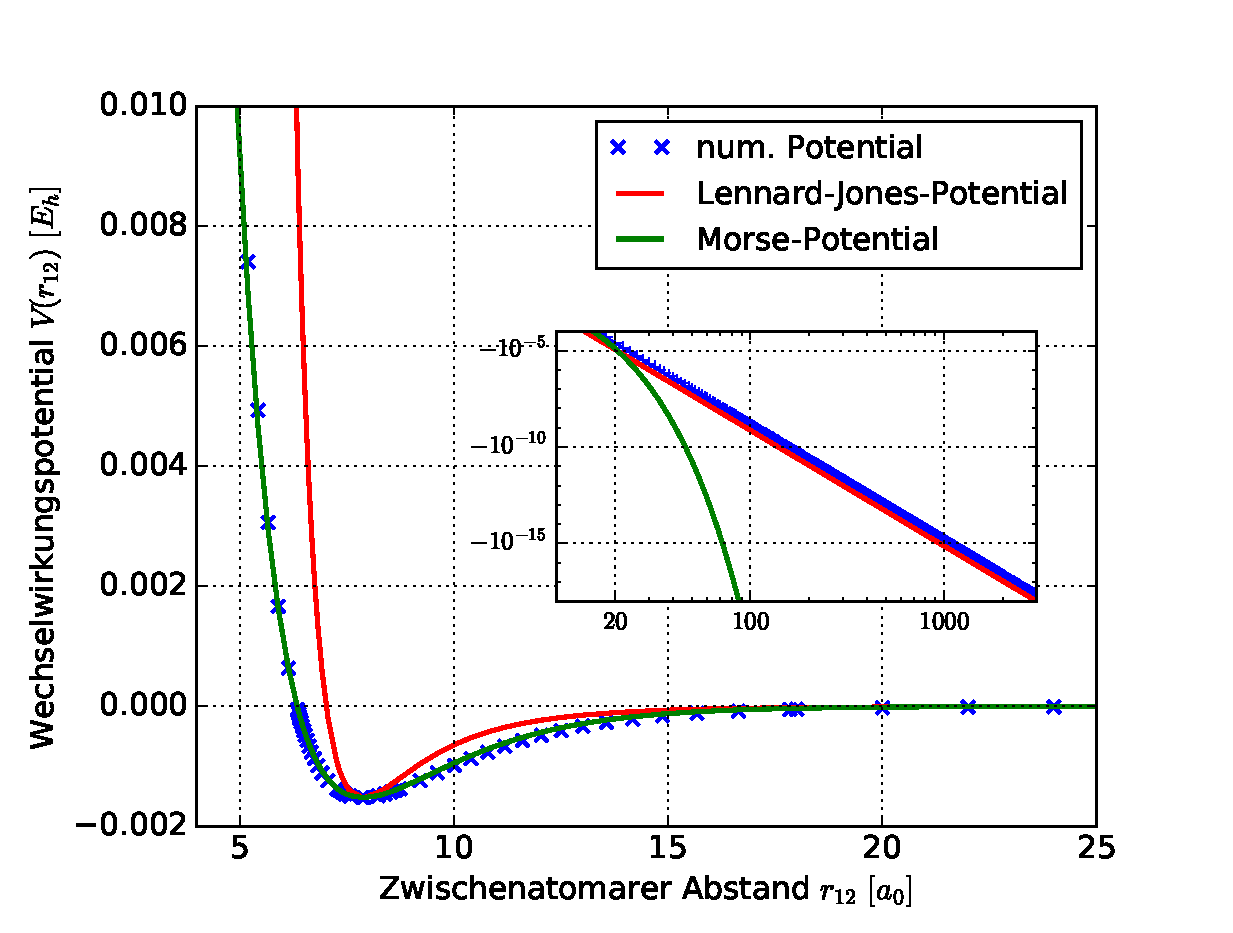
\includegraphics[scale=0.7]{WW.eps}
%	%	\vspace*{-10mm}
%	\caption{Dargestellt ist ein numerisches Potential (blau, gekreuzt) eines 
%	angeregten Tripletzustandes des $^7$Li$^7$Li Systems und 
%	zwei 
%	Näherungsfunktionen: das Morse-Potential (grün) und das 
%	Lennard-Jones-Potential (rot). Im Sub-Plot sieht man das Verhalten für 
%	größere Abstände. Für die Parameter $D_e$ (Dissoziationsenergie) und $R_m$ 
%	(Lage des Minimuns) ist der Tiefpunkt der 
%	numerischen Kurve benutzt worden. Der Exponent des MRPs 
%	wird zu 
%	$a_\text{st}=0.45$ 
%	gewählt.}
%	%\vspace{2mm} %\hrule 
%	\label{pic:Pot} 
%\end{figure}
%
In \ref{pic:Pot} ist zu sehen, dass das MRP im Bereich von 5-20 $a_0$ eine sehr 
gute Näherung 
darstellt, wogegen das LJP in diesem Bereich kaum dem numerischen Potential 
folgt. Für Abstände größer als 20 $a_0$ hingegen fällt das 
MRP deutlich zu 
schnell ab. Schon bei einem Abstand von ungefähr 100 $a_0$ erreicht es schon 
die Rechnergenauigkeit und wird auf 0 gerundet. Das LJP nähert sich dagegen der 
numerischen Kurve weiter an und 
folgt der Kurve 
über mehrere Größenordnungen des Abstandes. Lediglich ein leichter Off-set ist 
zu erahnen. An dieser Stelle sei erwähnt, dass die hier 
dargestellte Näherung 
nur durch optische Anpassung gewonnen wird. Es ist zu 
erwarten, dass eine 
numerische Anpassung (Fit) ein besseres Ergebnis auf Kosten 
einer 
Nichtübereinstimmung im Minima liefern kann.  \\

Das MRP besitzt den großen Vorteil einer vollständigen Beschreibung und 
Berechnung ohne den Bedarf einer Renormierung. Dagegen beschreibt das LJP die 
physikalische Gegebenheit besser und für große Abstände auch quantitativ 
genauer. Mithilfe des freien Parameters im Exponenten 
kann jedoch das MRP die Kurve nahe am Ursprung besser beschreiben. \\

Ziel der Betrachtung ist es, die Bemühung einer Renomierung des bekannten 
$\delta$-Pseudopotentials als Wechselwirkungspotential zu umgehen, indem ein 
realistisches Potential verwendet wird. Erhofft wird eine bessere Berechnung 
mittels CI von ultrakalten Gasen. Durch Nutzung des LJP und 
des 
Algorithmus kann zwar ein realistisches bzw. 
realistischeres\footnote{da das 
LJP dennoch eine Näherungsfunktion ist} Potential als das 
$\delta$-Potential 
verwendet werden, jedoch auf Kosten einer neuen 
Renormierung\footnote{Renormierung der Basisintegrale}. Dementsprechend 
erfüllt das LJP nicht ganz die erwarteten Eigenschaften. 
Dagegen ist das MRP 
mathematisch angenehmer und es ist keine Renormierung nötig. \\
Das MRP ist ebenfalls ein realistischeres Wechselwirkungspotential als das 
$\delta$-Potential, auch wenn es für große Abstände deutlich zu schnell 
abfällt. 
Dennoch soll es möglich sein, die relevanten Eigenschaften 
mittels MRP 
darzustellen und herauszufinden, ob eine CI-Rechnung 
prinzipiell möglich sei 
und ob diese eine Verbesserung liefere. Das MRP divergiert 
zwar nicht in 0, 
nimmt aber sehr große Werte an. Es kann daher passieren, dass im Rahmen der 
Integration zwar Ergebnisse produziert werden, diese aber unphysikalisch groß 
sind. Dieses Verhalten muss durch geeignete Wahl der Basisfunktionen der 
CI-Rechnung berücksichtigt werden.   \\

Weiterhin sei hier erwähnt, dass es auch Mischformen dieser Potentiale gibt. 
Vorstellbar ist, dass das Potential
%
\begin{align}
V\propto e^{-a_\text{st}\cdot r}-\rl{\frac{R_m}{r}}^6 \quad,
\end{align}
%
auch (modifiziertes) Buckingham-Potential genannt (siehe z.B. in \cite{av:2b} 
oder 
\cite{av:3b}), eine noch bessere 
Beschreibung über den gesamten Bereich der Abstände liefert und die guten 
Eigenschaften beider Potentiale vereint. Ohne weitere Untersuchung kann auf 
zwei Tatsachen hingewiesen werden: Zum einen muss auch dieses 
Potential für 
einige Fälle im Rahmen des oben beschriebenen Algorithmus renormiert werden, 
jedoch seltener als das LJP. Zum anderen 
beinhaltet dieses Potential den $\frac{1}{r^6}$ -Term und wird daher die 
Eigenschaft des LJP erben, sodass große Abstände gut 
beschrieben werden können.
%
%
%
%%
\chapter{Implementierung}\label{sec:Implementierung}
%
In diesem Kapitel wird eine Implementierung des Algorithmus inklusive 
der 
Anpassungen an das Wechselwirkungsproblem dargestellt, getestet und auf weiter 
Optimierungsmöglichkeiten sowie bestehende Probleme hingewiesen. Es wird die 
Programmiersprache FORTRAN auf dem Standard von FROTRAN 90 verwendet. 
Weiterhin 
kommen kleinere Programme aus der NAG - Bibliothek \cite{o:1a} und der 
Numerical 
Recipes \cite{b:4a} zum Einsatz; entsprechende Abschnitte sind hier 
und im Quellcode gekennzeichnet. Das Programm wird der Arbeitsgruppe zur 
Verfügung gestellt. 
%
%
%
\section{Integralberechnung mit \texttt{gto\_int}}
%
Für eine spätere Verwendung in einer CI Rechnung ist die Subroutine 
\texttt{gto\_int} 
entworfen worden. Eingebettet ist diese in dem Programm 
\texttt{gto\_int\_test}, 
welches hier 
nicht weiter erläutert wird, da es lediglich zum Aufruf und Testen 
dient. 
Weiterhin solle erwähnt werden, dass hier nur der ausführende Teil 
der 
Implementierung erklärt wird. Etwaige Kommentarfunktionen, In- und 
Output-Programmteile oder Abschnitte zur Fehlerbehebung werden ausführlich in 
einer zusätzlichen Dokumentation erklärt bzw. verfügbar sein.    
%
%
%
\subsection{Programmablauf, Subprogramme und Funktionen}
%
\texttt{gto\_int} stellt die Zusammenfassung aller im Abschnitt 
\ref{sec:Zusammenfassung:Algorithmus} erwähnten Teilschritte zur 
Berechnung des 
Integrals dar. Es sind bisher zwei Typen an 
Wechselwirkungspotentialen 
berücksichtigt, Lennard-Joens-artige Potentiale (??), das heißt 
Wechselwirkungen, 
die mit 
Potenzen des Abstands gehen und Morse-Potential-artige Wechselwirkungen, die 
aus einer Summe zweier Exponentialfunktionen des Abstandes gehen. Der Aufruf 
der Routine kann mithilfe von
%
\begin{lstlisting}
CALL gto_int(i1,i2,j1,j2,k1,k2,l1,l2,m1,m2,n1,n2,a,b,c,d, &
           & vecA,vecB,vecC,vecD, & 
           & pot_par1,pot_par2,pot_par3,pot_par4,pot_par5,pot_OP,&
           & pot_name, I )
\end{lstlisting}
%
geschehen. \texttt{i1-n2} sind die Potenzen der Monome der GTOs, \texttt{a-d} 
die 
Exponenten und 
\texttt{vecA-vecD} die Zentren. Anschließend kommen die Potentialparameter und 
der Rückgabewert des Integrals I. Im Folgenden werden Beispiele zur Anwendung 
der Potentialparameter gezeigt, jedoch soll die genaue Verwendung dem 
Quellcode oder der Dokumentation entnommen werden. An dieser Stelle 
ist eine 
Besonderheit der Implementierung zu erwähnen. Die Potentialtypen sind 
allein 
durch ihre Struktur gegeben. Durch die entsprechende Wahl der Parameter 
können auch 
noch nicht direkt diskutierte Potentiale verwendet werden. \\ Zwei Beispiele:
%
\begin{enumerate}
	\item Wird das  "(0,0)-LJP"\ genutzt und die Konstanten 
	$A_\text{LJP}=1$ 
	und 
	$B_\text{LJP}=0$ gesetzt (vgl. \ref{eq:def:LJP}), entsteht das 
	Potential
	\begin{align}\label{eq:def:V1}
	V_1 = \frac{1}{r_{12}^0}+\frac{0}{r_{12}^0}\equiv 1 \quad,
	\end{align}
	welches dem trivialen Potential bzw. keiner Wechselwirkung 
	entspricht. Nach Konstruktion des Integrals \ref{eq:2T-Integrale} 
	unter 
	Zuhilfenahme der GTOs kann hierdurch auch das Produkt der Normen 
	berechnet werden. Aufgerufen 
	kann ein solches Potential mit den 
	Potentialparametern\footnote{alle 
	Potentialparameter müssen den Datentyp \texttt{real(KIND=8)} haben}:\\
	\texttt{pot\_par1}=0 und \texttt{pot\_par2}=0 für die Potenzen der 
	Abstände, 
	\texttt{pot\_par3}=1 und 
	\texttt{pot\_par4}=0 für die Konstanten und \texttt{pot\_OP}=1.\\
	\texttt{pot\_par5} wird nicht benötigt, kann also beliebig gesetzt werden. 
	Unter 
	Option 1 (\texttt{pot\_OP}) wird \texttt{pot\_par5} auch nicht weiter 
	verwendet. \texttt{pot\_name} 
	muss dem 3 
	stelligen Charakter "\texttt{LJP}"\ entsprechen.
	%
	\item Wird das "(-2,0)-LJP"\ genutzt, das heißt analog \texttt{pot\_par1}=2 
	und 
	\texttt{pot\_par2}=0, mit dem selben Konstanten wie zuvor, entspricht das 
	einer 
	quadratischen Wechselwirkung:
	\begin{align}\label{eq:def:V2}
	V_2(r_{12})=\frac{1}{r_{12}^{-2}}+\frac{0}{r_{12}^0}=r_{12}^2\quad.
	\end{align}
\end{enumerate}
Diese Beispiele zeigen den prinzipiell großen Spielraum bzgl. des 
Potentials. 
Dennoch wird darauf Rücksicht genommen, dass beliebig viele weitere 
Potentiale 
hinzugefügt werden können. Die in diesem Beispiel dargestellten 
Potentiale 
werden im Abschnitt \ref{sec:T:norm} und \ref{sec:T:quad} noch einmal 
benötigt.\\

Das folgende Diagramm zeigt den konzeptionellen Ablauf der Subroutine 
gto\_int.
%
\begin{figure}[H] \centering
	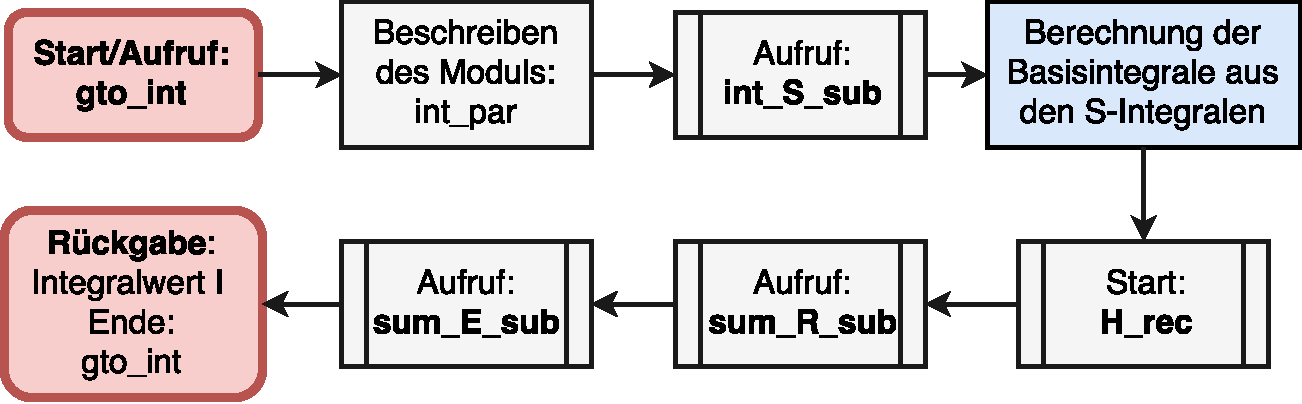
\includegraphics[scale=0.7]{gto_int.pdf}
	%	\vspace*{-10mm}
	\caption{Programmablaufplan der Subroutine \texttt{gto\_int}}
	\vspace{2mm} %\hrule 
	\label{pic:FC:gto_int} 
\end{figure}
%
Das Modul \texttt{int\_par} stellt eine Sammlung aller für das Integral 
wichtigen 
Parameter, wie zum Beispiel Exponenten der GTOs oder die erwähnten 
Potentialparameter\footnote{Der Programmteil des Beschreibens von 
\texttt{int\_par}, das 
Modul \texttt{int\_par} selbst und die Berechnung der Basisintegrale aus den 
S-Integralen
müsste angepasst werden, um weitere Potentialtypen hinzuzufügen.}, für alle 
weiteren Teilprogramme bereit. 
\texttt{int\_S\_sub}, \texttt{H\_rec}, \texttt{sum\_R\_sub} und 
\texttt{sum\_E\_sub} sind Teilprogramme, die im 
Folgenden noch näher beschrieben werden. Programmschritt 3 (Berechnung der 
Basisintegrale $\Pi_j^\pm$) wird je nach gewähltem Potential mit Formel 
\ref{eq:PIinS_MRP} bzw. \ref{eq:PI_LJP} durchgeführt.
%
%
%
\subsubsection{$S$ Integrale mit \texttt{int\_S\_sub}}
%
Einer der ersten Schritte ist die Berechnung der S-Integrale \ref{eq:def:S}. Je 
nach Potential kann $\alpha$ positiv, als auch negativ sein und so in das 
Renormierungschema \ref{sec:renorm} rutschen. Weiterhin muss immer eine Schar 
an Integralen berechnet werden, für jedes j der $\Pi^\pm_j$-Integrale. Daher 
wird \texttt{int\_S\_sub} derart designt, dass zu einem gegebenen maximalen j 
und 
gegebenen Potentialtyp ein Vektor aller benötigten S-Integrale ausgegeben wird.
Ausgehend vom Potentialtyp wird zunächst $\alpha$, mit der Obergrenze von j, 
$\beta$ und $\gamma$ berechnet. Weiterhin kann die Untergrenze (j=1) von 
$\alpha$ angegeben werden; diese Größe soll nun $\alpha_s$ heißen. Anschließend 
treten die Größen
\begin{align}\label{eq:def:parameter y,x}
y=\frac{\beta^2}{4 \gamma}= \xi Q^2 \quad\text{und}\quad 
x=\frac{\gamma}{\beta^2}=\frac{1}{4y}=\frac{1}{4\xi Q^2}
\end{align}
häufig auf und können gut zur Unterscheidung pathologischer Fälle genutzt 
werden.
%
\begin{figure}[H] \centering
	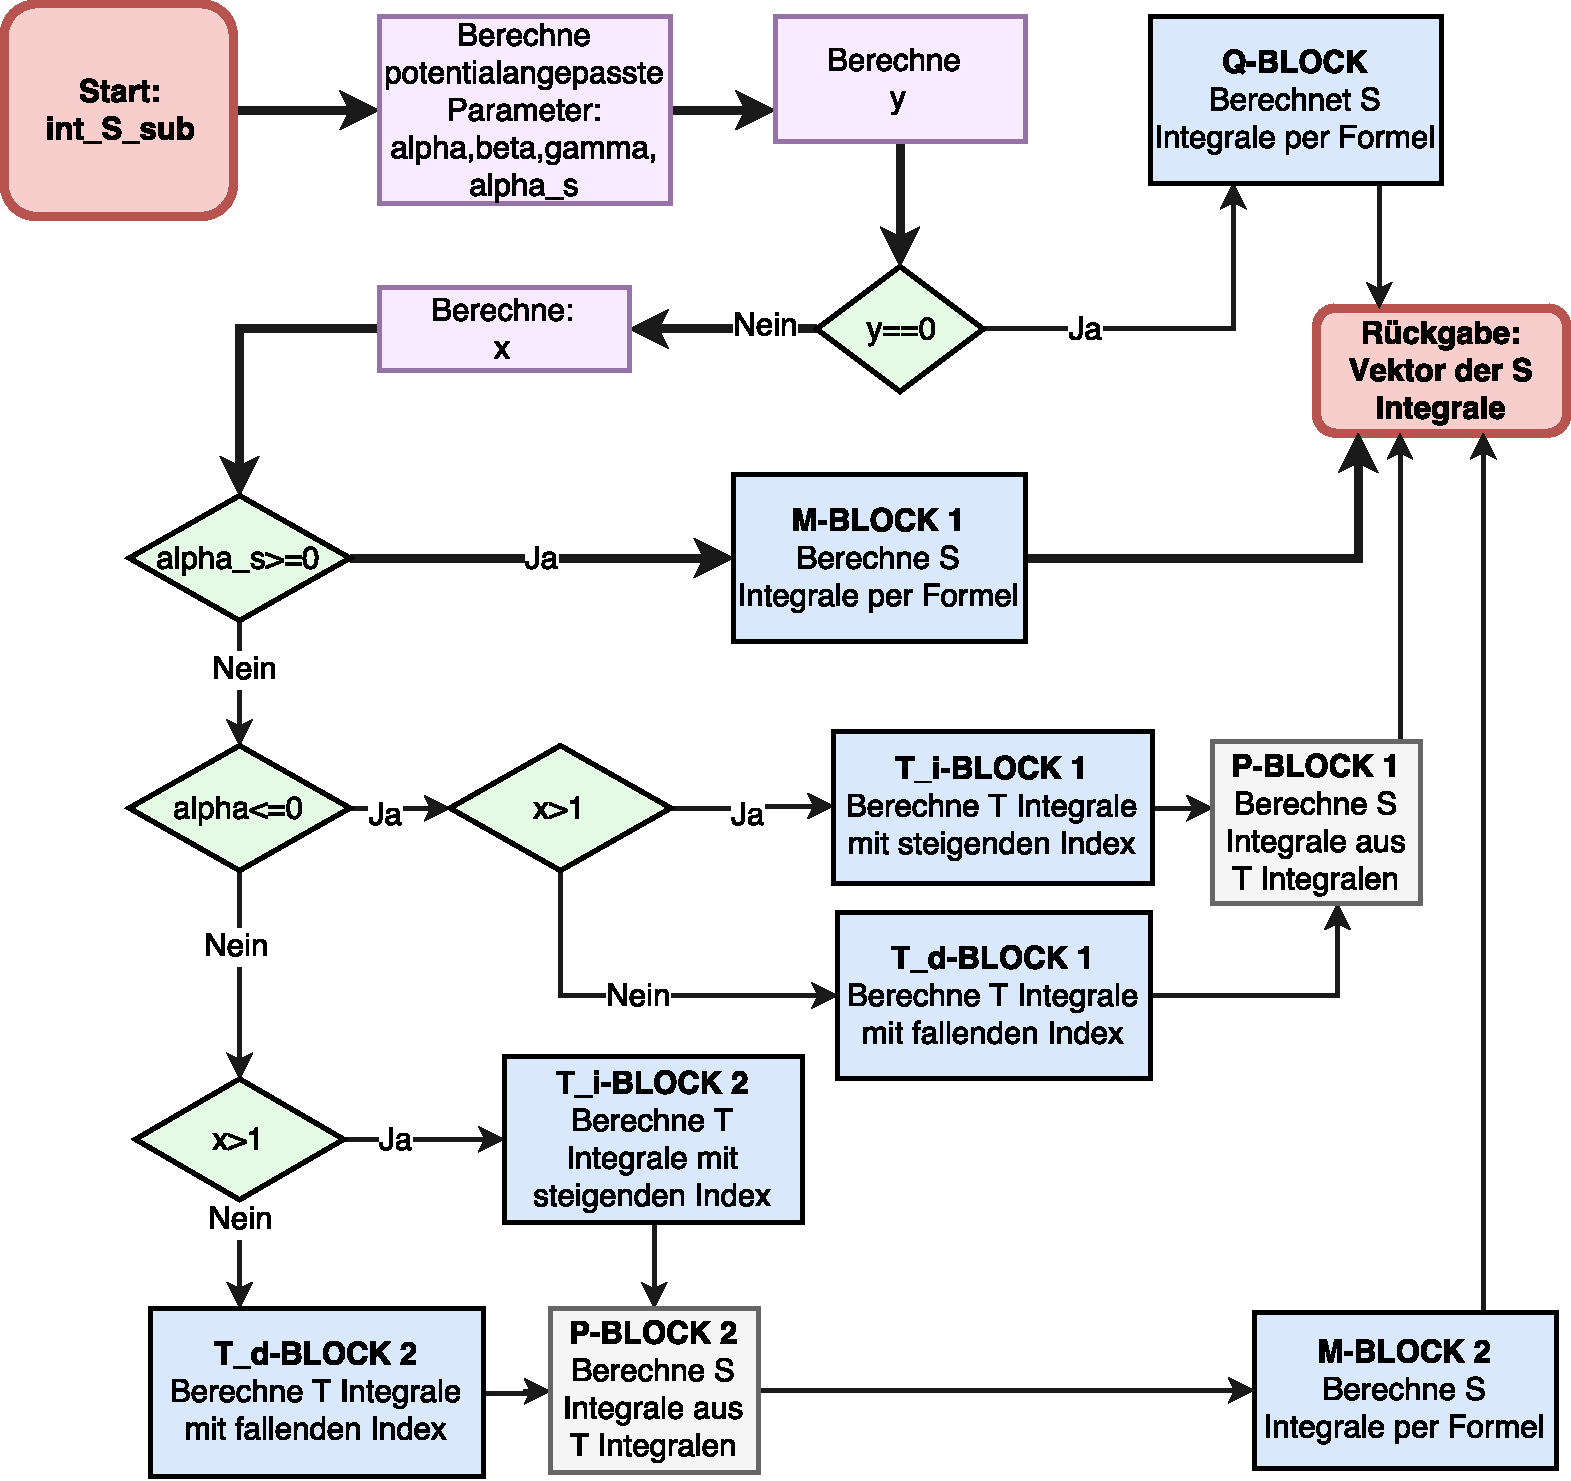
\includegraphics[scale=0.59]{int_S_sub.pdf}
	%	\vspace*{-10mm}
	\caption{Programmablaufplan der Subroutine \texttt{int\_S\_sub} zur 
	Berechnung der 
	Integrale \ref{eq:def:S} mit der Möglichkeit der Nutzung des 
	Renormierungschemas in Abschnitt \ref{sec:renorm}. Dick markiert ist der 
	Pfad ohne Nutzung einer Renormierung (Standard Pfad).}
	\vspace{2mm} %\hrule 
	\label{pic:FC:int_S_sub} 
\end{figure}
%TODO pagebreak in finaler version
%
Wie in Abbildung \ref{pic:FC:int_S_sub} zu sehen, enthält \texttt{int\_S\_sub} 
verschiedene Berechnungsblöcke. Folgende Auflistung beschreibt kurz ihren 
jeweiligen Zweck:
%
\begin{enumerate}
	\item \textbf{M-Block 1} berechnet für alle j die S-Integrale mithilfe der 
	Formel 
	\ref{eq:S,alpha>0}. Alle $\alpha(j)$ sind positiv, da $\alpha_s \geq0$ 
	(kein Renormierungsschema).
	%
	\item \textbf{M-Block 2} berechnet ein Teil der S-Integrale für alle j mit 
	$\alpha(j)>0$ mit Formel \ref{eq:S,alpha>0} (kein Renormierungsschema). 
	%
	\item \textbf{T\_i-Block 1/2} berechnen unter Zuhilfenahme des 
	Renormierungsschemas in \ref{sec:renorm} die T-Integrale \ref{eq:def:T-Int} 
	mit wachsenden Index $s=-\alpha(j)$ in der Rekursion \ref{eq:recursivT}.
	%
	\item \textbf{T\_d-Block 1/2} berechnet unter Zuhilfenahme des 
	Renormierungsschemas in \ref{sec:renorm} die T-Integrale \ref{eq:def:T-Int} 
	mit fallenden Index $s=-\alpha(j)$ in der Rekursion \ref{recursiveT2}.
	%
	\item \textbf{P-Block 1/2} berechnet die S-Integrale für negative $\alpha$ 
	aus den T-Integralen durch Formel \ref{eq:SinT}.
	%
	\item \textbf{Q-Block} berechnet S-Integrale für Q==0. Dadurch vereinfacht 
	sich das Integral enorm und kann fast ausschließlich durch Fakultäten 
	berechnet werden. Für negative $\alpha(j)$ wird das Renormierungsschema 
	\ref{sec:renorm} analytisch angewandt. Da für die Verwendung in 
	\texttt{gto\_int} Q 
	nie 0 sein wird, da hier der Algorithmus nicht funktioniert (siehe zum 
	Beispiel \ref{eq:Hobson}), werden die Formeln für diesen Block lediglich in 
	der Dokumentation stehen. Weiterhin sei erwähnt, dass dieser Block zur 
	Fehlerbehebung und der Vollständigkeit halber implementiert wird; 
	\texttt{int\_S\_sub} kann damit auch in anderen Programmen wiederverwendet 
	werden.
\end{enumerate}
%
Für das MRP und die Potentiale $V_1$ und $V_2$, welche keine Renormierung 
benötigen, wird nur der dick markierte Pfad verwendet.
%
%
%
\subsubsection{Rekursive Funktion \texttt{H\_rec} für $\mathcal{H}_{11l}^\pm$}
%
%
\begin{figure}[H] \centering
	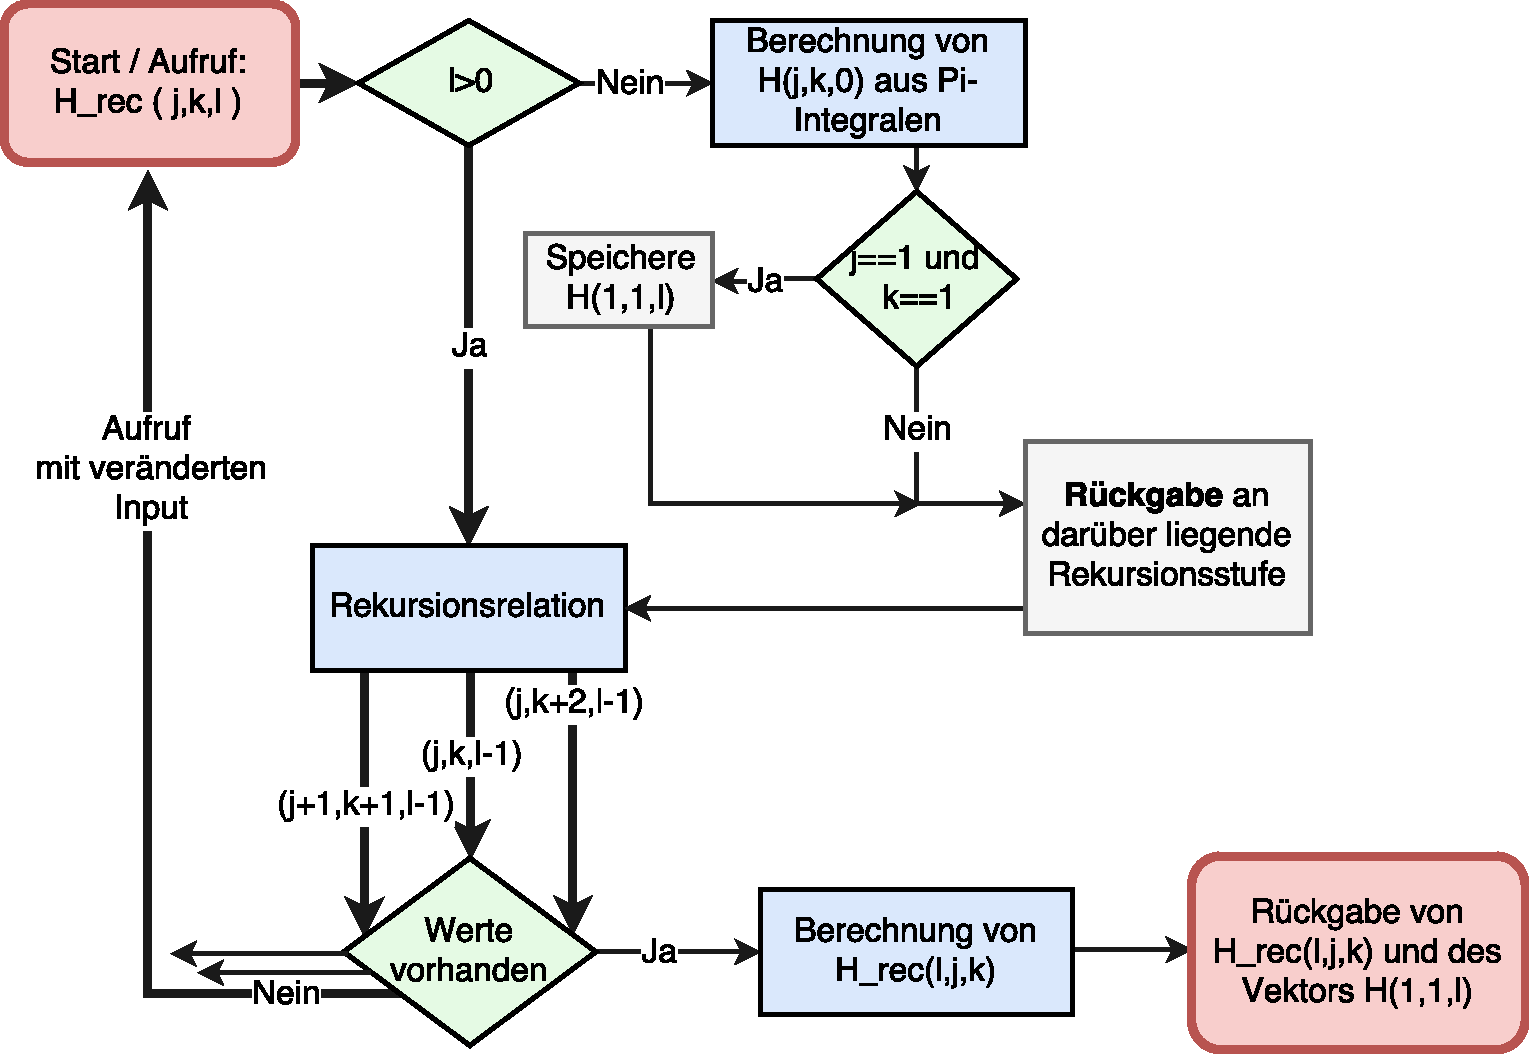
\includegraphics[scale=0.55]{H_rec.pdf}
	%\vspace*{-10mm}
	\caption{Programmablaufplan der rekursiven Funktion \texttt{H\_rec}  unter 
		Verwendung der Formeln \ref{eq:rek:H}  und \ref{eq:prop:H}. Pfade, die 
		auf 
		den Start zurückführen, bedeuten einen rekursiven Aufruf mit 
		veränderten 
		Input. Der dick markierte Pfad zeigt die Rekursionsschleife.}
	%\vspace{2mm} %\hrule 
	\label{pic:FC:H_rec} 
\end{figure}
%
Mithilfe der in \texttt{gto\_int} (unter Verwendung der S-Integrale) 
berechneten 
$\Pi^\pm_j$-Integralen wird nun die Rekursion \texttt{H\_rec} durchgeführt.
Die zentrale Formel hierbei ist die Rekursionsrelation \ref{eq:rek:H}.\\
%
 Abbildung 
\ref{pic:FC:H_rec} zeigt den konzeptionellen Ablauf der Funktion. Führt ein 
Pfad zurück auf das Startfeld, so bedeutet dies einen rekursiven 
Aufruf. Wird ein Ergebnis in der tiefsten Rekursionsstufe (l=0) berechnet, 
führt das zu einer Rückgabe des Werts an die Rekursionsrelation und damit zu 
einer Berechnung der darüber liegenden Stufe. Die Abfrage "Werte vorhanden"\ 
ist keine im Quellcode ersichtliche Programmstelle, sie veranschaulicht hier
lediglich die Funktionsweise eines rekursiven Aufrufs. Weiterhin wird darauf 
hingewiesen, dass diese Rekursion mit dem maximalen Indizes gestartet wird. Im 
Laufe der Rekursion werden dabei alle Fälle mit j=1 und k=1 mit beliebigen l in 
ein 
Vektor gespeichert. So kann sichergestellt werden, dass alle 
benötigten Werte für den nächsten Schritt (Formel \ref{R_sum}) bereit stehen. 
Zusätzlich ist in Abbildung \ref{pic:FC:H_rec} ersichtlich, dass bei jeder 
Rekursionsschleife drei 
Aufrufe der Funktion folgen. Da in jeder Stufe l um 1 reduziert wird, 
ergeben 
sich $3^l$ rekursive Aufrufe. l ergibt sich, wie in  Abschnitt über 
\ref{eq:final:Hobson} zu sehen, aus 
der Summe aller Potenzen der Monome der GTOs. Da in der Praxis 
selten höher als d-Orbitale betrachtet werden, sind Werte größer als $l=4\cdot 
(2+2+2)=24$ nicht 
zu erwarten. Dennoch ist die daraus resultierende Anzahl\footnote{für vier GTOs 
in 
d-Orbitalen, dh. l=24 folgen $3^{24}=282429536481\approx3\cdot 10^{11}$ 
rekursive Aufrufe der Funktion \texttt{H\_rec}} der Funktionsaufrufe sehr 
hoch und kann prinzipiell zu Fehlern führen. Daher wird an dieser Stelle auf 
potentielle Laufzeitprobleme oder Rundungsfehler für hohe Orbitale hingewiesen.
%
%
%
\subsubsection{Subroutine \texttt{sum\_R\_sub}}
%
Die Subroutine \texttt{sum\_R\_sub} soll nun alle relevanten kartesischen 
Ableitungen des Basisintegrals unter Anwendung des Hobson Theorems berechnen. 
Die schon in Kapitel 
\ref{sec:Algorithmus} dargelegte Formel \ref{R_sum} 
führt diesen Schritt auf eine Summe über die radialen Ableitungen 
$\mathcal{H}_{11l}$ zurück. Eine erste Optimierung dieser Berechnung zeigt 
sich, wenn auf die richtige Berechnungsreihenfolge der Summen geachtet wird. 
Die m-Summe 
und die k-Summe sind unabhängig voneinander und müssen somit nicht 
geschachtelt berechnet werden. Es gilt also
%
\begin{align}\nonumber
R^{\tau,\rho,\sigma}&=\sum_{l=0}^{l_{max}} 
%
\underset{=:R_m(\,l\,;\,c^{-1},Z)}{\underbrace{\sum_{m=-l}^{l}c^{-1}(l,m,\tau,\rho,\sigma)Z_{lm}(\textbf{Q})}}
%
\underset{=:R_k(l\, ;\, 
\mathcal{H}^\pm_{11l},d,Q)}{\underbrace{\sum_{k=0}^{k_{max}}d_k^{l,k_{max}} 
\cdot 
\left[(\mathcal{H}^-_{11l}-\mathcal{H}^+_{11l})\right]Q^{l_{max}-l-2k}}}\\\label{eq:short_R_sum}
%
&=\sum_{l=0}^{l_{max}}R_m(l)\cdot R_k(l)\qquad,
\end{align}
%
wobei ($\tau,\rho,\sigma$) für alle möglichen  Kombinationen der Potenzen der 
Ableitungen stehen. Die maximalen Werte können an Gleichung \ref{eq:E:Koef} 
abgelesen werden.\\
Für die Implementierung ist weiterhin wichtig:
\begin{enumerate}
	\item alle Werte von ($\tau,\rho,\sigma$) abzulaufen (die ersten "drei"\  
	Schleifen, die mit den Indizes t,u,v gekennzeichnet sind, vlg. 
	\ref{eq:E:Koef} bzw. Abbildung \ref{pic:FC:sum_R_sub}).
	%
	\item die im Abschnitt \ref{sec:Hobson_schlegel} 
	erwähnte, aus \cite{av:9a} stammende Bedingung, dass $c^{-1}\equiv0$ ist, 
	falls $l-l_{max}$ ungerade wird, zu berücksichtigen.
	\item die zwei unabhängigen Summen $R_m(l)$ und $R_k(l)$ separat und nicht 
	geschachtelt zu berechnen.
	\item d und $c^{-1}$ Koeffizienten möglichst außerhalb der 
	Schleifenstruktur vorher zu berechnen, um Funktionsaufrufe zu minimieren. 
\end{enumerate}
%
\begin{figure}[H] \centering
	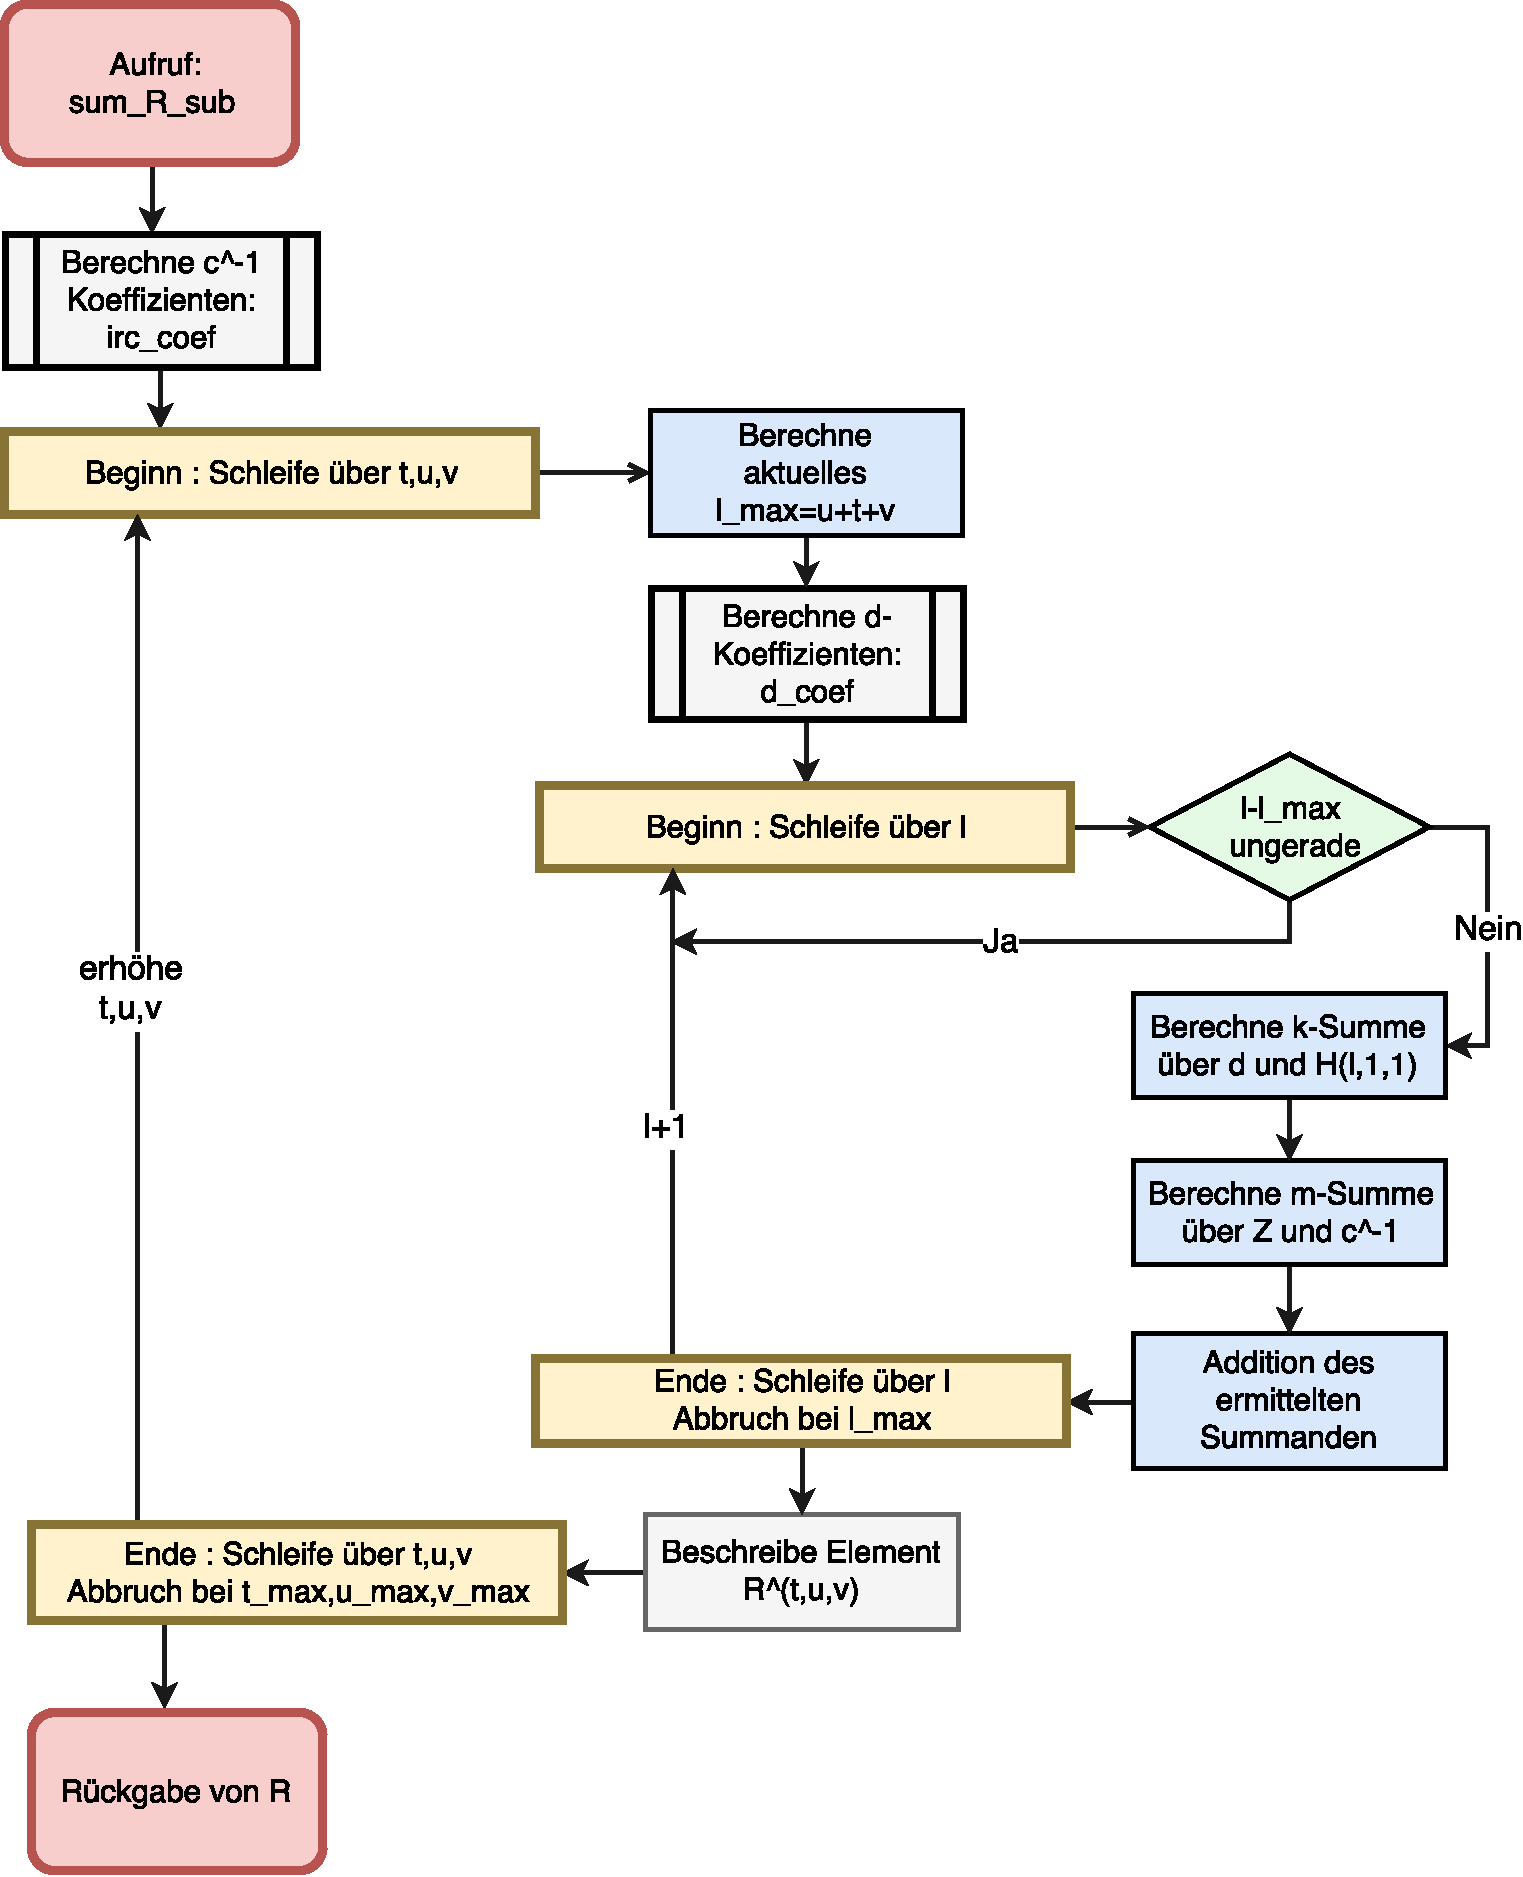
\includegraphics[scale=0.6]{sum_R_sub.pdf}
	%\vspace*{-10mm}
	\caption{Programmablaufplan der Subroutine 
	\texttt{sum\_R\_sub}. 1. Schleife geht über alle 
	Einträge von R, die 2. Schleife summiert über l 
	vlg. Formel \ref{eq:short_R_sum}. Die Summen über k 
	und m sind in den blauen 
	Blöcken rechts zusammengefasst.}
	%\vspace{2mm} %\hrule 
	\label{pic:FC:sum_R_sub} 
\end{figure}
%
Zurückgegeben wird ein 3d-Feld $R^{\tau,\rho,\sigma}$, 
welches in der Routine \texttt{sum\_E\_sub} wiederverwendet 
wird. Bevor diese erläutert wird, 
sollen kurz die Subroutinen zur Berechnung der Koeffizienten skizziert werden.
%
\subparagraph{Zur Berechnung der d-Koeffizienten mit \texttt{d\_coef}}
%
wird Formel \ref{eq:rek_d} benutzt. $d^{l,k_{max}}_{k}$ hat drei freie 
Parameter; sobald $l_{max}$ festgelegt ist (vgl. 
Abbildung 
\ref{pic:FC:sum_R_sub} ), kann d als Matrix der 
Ausdehnung $l_{max}\times k_{max}$ aufgefasst werden. Die 
Subroutine geht dabei folgende Schritte durch:
\begin{enumerate}
	\item Gehe alle möglichen Zahlen für l und k durch.
	\item Starte für die gegebene Kombination von l, k die Rekursion 
	\ref{eq:rek_d} , welche durch die Funktion \texttt{d\_rec} realisiert ist.
	\item Speichere das Ergebnis in der Matrix d(k,l).
\end{enumerate} 
Diese Matrix wird anschließend an \texttt{sum\_R\_sub} zurückgegeben. 
%
%
%
\subparagraph{Die Berechnung der $c^{-1}$-Koeffizienten mit \texttt{irc\_coef}}
%
benutzt in erster Linie die Gleichung \ref{eq:def:c_koef}. Zu erkennen ist 
jedoch, dass dazu die c-Koeffizienten benötigt werden. Die Formel für diese 
wird der Arbeit \cite{av:4a} entnommen, wobei jedoch auch hier kleinere 
Tippfehler vorhanden sind. Im Anhang \ref{sec:AnhangA:Schlegel} sind alle 
benötigten Formeln bzgl. c und der damit verbundenen Transformation richtig 
gestellt und angegeben.  Weiterhin sind dort noch weitere Anmerkungen zur 
Implementierung vorhanden. %(??)
%
%
%
\subsubsection{Subroutine \texttt{sum\_E\_sub}}
%
Nachdem nun das Feld $R^{\tau,\rho,\sigma}$ bekannt ist, muss die Summe 
\ref{eq:E:Koef}\  ausgeführt werden. Diese Summe wird durch die Subroutine 
\texttt{sum\_E\_sub} durchgeführt. Dazu werden die oben erwähnten Koeffizienten 
$E^{ij}_t$ (\ref{eq:E:coef1} - \ref{eq:E:coef4}) benötigt, welche mit der 
Subroutine \texttt{E\_coef} berechnet werden. Hier werden für gegebene Zahlen i 
und j 
alle t durchgegangen und anschließend die Rekursionen ab \ref{eq:E:coef4} 
gestartet. Diese Rekursionen sind in der Funktion \texttt{E\_rec} 
implementiert. Dabei 
unterscheidet \texttt{E\_rec} folgende Fälle:
\begin{enumerate}
	\item i=j=t=0 $\Rightarrow$ Gleichung \ref{eq:E:coef1}
	\item i,j,t < 0 oder t>i+j $\Rightarrow$ $E^{ij}_t=0$
	\item $t\neq0$ $\Rightarrow$ Gleichung \ref{eq:E:coef4}
	\item $t=0$ und $i\neq0$ $\Rightarrow$ Gleichung \ref{eq:E:coef2}
	\item $t=0$ und $i=0$ und $j\neq0$ $\Rightarrow$ Gleichung \ref{eq:E:coef3}
\end{enumerate}
Wobei \ref{eq:E:coef2} und \ref{eq:E:coef3} auf abfallende Index, das heißt 
$E^{i,j}_t(i-1,j,t)$,  umgeschrieben sind.   \\
Nachdem alle Koeffizienten bekannt sind, muss nun die Summe \ref{eq:E:Koef} 
ausgeführt werden. Diese wird durch 6 ineinander geschachtelte Schleifen 
realisiert. 
%
%
%
\subsubsection{Weitere mathematische Funktionen}
%
Neben den schon diskutierten Funktionen und Subroutinen werden noch einige 
kleinere mathematische Funktionen benötigt, um alle Rechnungen durchzuführen.  
\begin{enumerate}
	\item In \texttt{int\_S\_sub}, genauer in den T-Blöcken, muss im Rahmen des 
	Renormierungsschemas die Funktionen $\omega_1(x)$, $\omega_0(x)$ und die 
	Diagamma-Funktion $\psi_d$ für ganz und halbzahlige Integer ausgewertet 
	werden. Diese werden in den Funktionen  \texttt{w1}, \texttt{w0} und 
	\texttt{diagamm} realisiert und folgen im Wesentlichen der 
	Berechnungsmethode aus \cite{av:1a2} für positive x. Im Anhang 
	\ref{sec:AnhangB:T_Integral} sind die entscheidenen Formeln für die 
	Berechnung gegeben.
	\item Weiterhin wird in \texttt{int\_S\_sub} (in den M-Blöcken) die 
	konfluierte hypergeometrische Funktion M berechnet. Die entsprechende 
	Realisierung der Reihendarstellung \ref{eq:reihe_M_kon.hyp.geo} unter 
	Verwendung der Pochhammer-Symbole ist in den Funktionen 
	\texttt{con\_hyp\_geo\_M} und \texttt{PHS} bewerkstelligt.
	\item In \texttt{sum\_R\_sub} werden die reellen soliden 
	Kugelflächenfunktionen benutzt. Die Berechnung dieser läuft über die 
	assoziierten Legendrepolynome, die durch die Routine \texttt{plgndr} aus 
	\cite{b:4a} berechnet werden. Restliche Konstanten, Fallunterscheidungen, 
	der Radial- und der $\phi$-Anteil werden in der Funktion \texttt{rsSHS} 
	bearbeitet. Nötige Definitionen und Konversionen sind im Anhang 
	\ref{sec:AnhangA:Schlegel} angegeben. 
    \item Allgemein werden Binomialkoeffizienten und Fakultäten benötigt. Dafür 
    benutzt man in erster Linie die Routinen \texttt{factrl} und \texttt{bico} 
    aus 
    \cite{b:4a}. Hinzu kommt die Funktion \texttt{cfact}, welche eine 
    Berechnung  eines Bruches von Fakultäten gekürzt berechnet 
    ($\frac{10!}{8!}=10\cdot 9$).
\end{enumerate}
%
%
%
\section{Genauigkeitstests}
%
In diesem Abschnitt soll auf verschiedene Weisen die Genauigkeit des Programms 
getestet werden. Dazu wird unter anderem eine Subroutine der NAG Bibliothek 
genutzt. Unter \cite{o:1a} kann die Dokumentation der genutzten Routine 
\texttt{D01FCF} 
abgerufen werden. \texttt{D01FCF} ist in der Arbeitsgruppe verfügbar und löst 
das 
sechsdimensionale Integral durch adaptive Quadratur über Hyperrechtecke. Die 
im Folgenden verwendete Größe ACC gibt die intern geschätzte Genauigkeit der 
NAG-Routine an. Weiterhin sei darauf hingewiesen, dass 
sich sprachlich auch in diesem Abschnitt auf die 
physikalische Gegebenheit bezogen wird, aber keinerlei 
Einheiten angegeben werden, da es sich dennoch um eine 
rein mathematische Betrachtung handelt. So wird zum 
Beispiel der später zu variierende Parameter $A_x$ als 
Abstand bezeichnet, um so die Benennung/ Unterscheidung zu 
vereinfachen und den späteren Bezug zur Physik nicht zu 
vergessen.
%
%
%
\subsection{Normberechnung ($f_{12}\equiv 1$)}\label{sec:T:norm}
%
Der erste Test den man an dem Programm durchführen kann, ist das 
Wechselwirkungspotential 1 zu setzen. Für nicht normierte GTOs ergibt sich 
mit dem Potential \ref{eq:def:V1} :  $f_{12}=V_1=1$ :
%
\begin{align*}
I&=\int\int\ d\textbf{r}_1\ d\textbf{r}_2 
(\psi_i^a(\textbf{r}_1)\psi_i^c(\textbf{r}_2))^*\cdot  1 \cdot  
\psi_j^b(\textbf{r}_1)\psi_j^d(\textbf{r}_2)\\
& =\int\ d\textbf{r}_1  \cdot 
x_{1,A}^i\,y_{1,A}^k\,z_{1,A}^m\cdot  
x_{1,B}^j\,y_{1,B}^l\,z_{1,B}^n\cdot e^{-b r_{1,B}^2-a 
	r_{1,A}^2} \cdot \\
&\qquad  \cdot \int\ d\textbf{r}_2\   
x_{2,C}^{i'}\,y_{2,C}^{k'}\,z_{2,C}^{m'} \cdot  
x_{2,D}^{j'}\,y_{2,D}^{l'}\,z_{2,D}^{n'}\cdot e^{-c r_{2,C}^2-d 
	r_{2,D}^2}\qquad.%\\
%&= N_{ikm}(a)N_{jln}(b)N_{i'k'm'}(c)N_{j'l'n'}(d) \qquad.
\end{align*}
%
Einfachheitshalber wird außerdem angenommen, dass 
%
\begin{align}\nonumber
\textbf{A}=\textbf{B} \quad&,\quad 
\textbf{C}=\textbf{D}\\\nonumber
a=b \quad&,\quad c=d\\\label{eq:tests:annahmen:norm}
(i,k,m)=(j,l,n) \quad&,\quad (i',k',m')=(j',l',n')
\end{align}
%
gilt. Damit wird das Integral zu
\begin{align}\label{eq:I_NORM}
I=I_\text{Norm}=N_{ikm}(a)^2 \cdot N_{i'k'm'}(c)^2 
\quad.
\end{align}
%
Diese Normen können durch die Formel \ref{eq:NORM} berechnet werden und stellen 
somit eine gute Überprüfungsmehtode dar. Die Berechnung 
beinhaltet weder 
kritische Summen noch relevante Funktionsaufrufe, die die Genauigkeit 
verschlechtern  könnten; das Ergebnis wird als wesentlich genauer als alle 
anderen Berechnungsmethoden angesehen.
%
\subsubsection{Variation des Orbitals}
%
Im Folgenden wird $(i',k',m')=(0,0,0)$ 
gesetzt und $(i,k,m)$ variiert. Es sei gesagt, dass der vertauschte Fall auch 
getestet wird und zu vergleichbaren Ergebnissen führt.  Weiterhin wird auf die 
Größe $l=2\cdot (i+k+m) $ hingewiesen. Die 2 entsteht durch die 
gegebenen Annahmen; allgemein ist l die Summe über alle Potenzen der GTOs. l 
gibt damit eine Charakteristik der Komplexität des Integrals an. 
Dementsprechend zeigen auch die folgenden Tests für unterschiedliche Orbitale 
mit gleichem l gleiche oder sogar höhere 
Genauigkeiten\footnote{Siehe dazu speziell die Orbitale 
(1,0,2) und (1,1,1) in Tabelle 
\ref{tab:norm:orbital}.}. Tabelle 
\ref{tab:norm:orbital} zeigt 
eine Auswahl der Testergebnisse, bei denen $A_x=1$, alle anderen Komponenten 0, 
\textbf{C}=\textbf{0} und a=c=0,001 konstant gesetzt worden ist.
%
\begin{table}[H] \centering
	\caption{Genauigkeitstest der Subroutine \texttt{gto\_int} 
	zu 
	verschiedenen 
	Orbitalen durch Normberechnung im Vergleich zu 
	analytischen Ergebnissen und 
	der numerischen NAG-Berechnung mit $A_x=1$ und 
	a=c=0,001.} \vspace{0.2cm}
	\begin{threeparttable} 
		\begin{tabular}{c|c||c||c||c}
			l&Orbital&  $I_\text{gto\_int}$            
			&  $I_\text{Norm}$     
			&$\left|\frac{I_\text{gto\_int}-I_\text{Norm}}{I_\text{Norm}}\right|$
			 \\ \hline\hline
			0&(0,0,0)&3,87578458503748E+09 & 
			3,87578458503748E+09 & 9,84E-16 \\
			2&(1,0,0)&9,68946146260323E+11 & 
			9,68946146259369E+11 & 9,85E-13 \\
			4&(0,0,2)&7,26709609873341E+14 & 
			7,26709609694527E+14 & 2,46E-10 \\
			6&(1,0,2)&1,81677760185790E+17 & 
			1,81677402423632E+17 & 1,97E-06 \\
			6&(1,1,1)&6,05592533952633E+16 &
			6,05591341412106E+16 & 1,97E-06 \\
			8&(2,0,2)&1,33465693978348E+20 & 
			1,36258051817724E+20 & 2,05E-02 
		\end{tabular}
		\vspace{4mm}
		\begin{tabular}{c|c||c||c|c||c}
			l&Orbital&  $I_\text{gto\_int}$ & 
			$I_\text{NAG}$           & ACC 
			[\%] & 
			$\left|\frac{I_\text{gto\_int}-I_\text{NAG}}{I_\text{gto\_int}}\right|$
			 \\ \hline\hline
			0&(0,0,0)&3,87578458503748E+09& 
			3,8757824E+09 & 3,87E-05 & 5,48E-07 
			\\
			2&(1,0,0)&9,68946146260323E+11& 
			9,6892021E+11 & 6,81E-05 & 2,67E-05 
			\\
			4&(0,0,2)&7,26709609873341E+14& 
			7,2670508E+14 & 8,91E-05 & 6,22E-06 
			\\
			6&(1,0,2)&1,81677760185790E+17& 
			1,8166964E+17 & 2,31E-04 & 4,47E-05 
		\end{tabular}
%		\begin{tablenotes}
		%	\item[I] 
%		\end{tablenotes}
	\end{threeparttable}
	\label{tab:norm:orbital}
\end{table}
%

In der Tabelle \ref{tab:norm:orbital} ist zu sehen, dass \texttt{gto\_int}, die 
NAG-Routine und die analytischen 
Berechnungen nach Formel \ref{eq:I_NORM} mithilfe der Norm vergleichbare Werte 
liefern. Das heißt, dass der Algorithmus prinzipiell funktioniert und die 
Implementierung in den hier gezeigten Fällen richtig ist. Im Vergleich zu der 
analytischen Berechnung zeigt sich, dass sich die relative Abweichung für ein 
höheres Orbital um 3-4 Größenordnungen verschlechtert. Zurückzuführen kann 
dieser Genauigkeitsverlust zum einen auf die Berechnung des Basisintegrals und 
zum anderen auf Rundungsfehler. Im Implementierungsstadium wird beobachtet, 
dass ein Basisintegral mit einem Fehler im wenigen Prozentbereich eine 
Ungenauigkeit von 6 Größenordnungen für das Integral mit sich führt, das heißt, 
dass dadurch
ein vollkommen falsches Ergebnis entsteht. Daher ist der Algorithmus sehr 
sensitiv auf Ungenauigkeiten des Basisintegrals. Dementsprechend kann 
vermutlich die Genauigkeit weiter erhöht werden, indem die Berechnung das 
Basisintegrals verbessert wird. Es soll daher erörtert werden, wie der in 
\cite{av:1a} und \cite{av:1a2} dargestellte Berechnungsweg von S ( Definition 
\ref{eq:def:S}) mithilfe der Tricomis konfluierten hypergeometrischen Funktion 
$\mathcal{U}$ korrigiert werden muss, um auch diesen verwenden zu können. 
Vorteil der dort dargestellten Berechnungsmethode ist, dass für 
unterschiedliche 
Intervalle der Eingabeparameter auch andere Berechnungsmethoden verwendet 
werden und so für 
einen größeren Bereich das Ergebnis die Genauigkeit beibehält. Im 
Falle von Rundungsfehlern bzw. Fehler, die durch 
Subtraktion zweier fast gleichgroßer Zahlen 
entstehen\footnote{z.B. in Formel \ref{eq:S,alpha>0} oder \ref{R_sum}
möglich}, 
kann untersucht werden, in welchem Programmteil diese 
aufkommen. Dafür nutzt man 
eine schon implementierte Debug-Funktion\footnote{Die Verwendung der 
detaillierten Ausgabe ist in der Dokumention erklärt.} im Programm. Im 
verantwortlichen Programmteil kann anschließend ein genauerer / 
höherer Datentyp (z.B. \texttt{REAL(KIND=16)} ) verwendet werden, um die 
Gesamtgenauigkeit zu erhöhen bzw. den Verlust von 
signifikanten Stellen zu verkleinern.\\

Weiterhin zeigt sich, dass im Vergleich zur NAG-Routine \texttt{gto\_int} ein 
vergleichbares bzw. besseres Ergebnis bis einschließlich l=6 erzeugt wird. Für 
l$\geq$8 soll \texttt{gto\_int} nicht mehr verwendet werden, 
da dort das Ergebnis kein Bezug mehr zum analytischen 
Ergebnis zeigt. Unter der Annahme, dass 
im Regime der ultrakalten Gase nur die einfachsten 
Orbitale eine Rolle spielen, 
kann man sich vorstellen, dass auch schon diese Stufe 
der Genauigkeit für die CI Rechnung 
ausreichen könnte. 

Die NAG-Routine hat unabhängig von l eine Genauigkeit 
von ungefähr $10^{-5}$ und kann nicht weiter gesteigert 
werden. Daher wird in diesem Abschnitt davon abgesehen, 
erneut mit der NAG-Routine zu vergleichen, da das 
analytische Ergebnis deutlich genauer ist.
%
\begin{table}[H] \centering
	\caption{Laufzeiten von \texttt{gto\_int} zu verschiedenen 
	Orbitalen. Es werden über 1000 Durchläufe 
	gemittelt.} \vspace{0.2cm}
	\begin{threeparttable} 
		\begin{tabular}{c|c||c}
		l&Orbital&Laufzeit [ms]\\ \hline
		0&(0,0,0)& 0,004\\
		2&(0,0,1)& 0,028\\
		2&(1,0,0)& 0,024\\
		4&(0,0,2)& 0,140\\
		6&(1,0,2)& 1,056\\
		8&(2,0,2)& 4,424\\
		10&(2,1,2)& 27,468\\
		12&(2,2,2)& 103,768\\
		\end{tabular}
		%		\begin{tablenotes}
		%	\item[I] 
		%		\end{tablenotes}
	\end{threeparttable}
	\label{tab:norm:orbital_time}
\end{table}
% 
Tabelle \ref{tab:norm:orbital_time} stellt Laufzeiten  
zu ihren Orbitalen dar. Dabei ist zu sehen, dass für 
ein höheres Orbital fast immer eine Größenordnung 
längerer Laufzeit benötigt wird. Für die sehr genau 
berechenbaren Integrale (l=\{0,2,4\}) werden nur rund 
0,2 ms benötigt, das heißt, es wären min. 5000 Integrale pro 
Sekunde möglich. Im Vergleich zu der NAG-Routine, die 
zwischen 87,404 s bis 93,052 s abhängig von l benötigt, 
ist \texttt{gto\_int} bis zu 5 Größenordnungen schneller. 
%
%
%
\subsubsection{Variation des Abstandes} 
\label{sec:var.Abstand_norm}
%
Nun soll das Orbital und die Exponenten konstant gehalten und der 
Abstand variiert werden. Die oben gewählten Annahmen 
\ref{eq:tests:annahmen:norm} bleiben weiterhin 
bestehen. An dieser Stelle sei nochmal darauf hingewiesen, dass der Algorithmus 
und damit das Programm nur für $Q\neq0$, das heißt für z.B.  
\textbf{A}=\textbf{B}$\neq$\textbf{C}=\textbf{D} funktioniert. 
(??) Dieser Fall entspricht einem Überlappintegral zwischen Orbitalen des 
selben 
Atoms oder zweier Orbitale von zwei Teilchen am selben Ort, was beides nicht 
vorkommen dürfte und daher auch nicht in dieser Arbeit betrachtet wird. \\
In diesem Test wird das Orbital $(i,k,m)=(1,0,0)$ und 
$(i',k',m')=(0,0,0)$ untersucht, da dieses ein 
repräsentatives, nicht triviales, aber dennoch sehr 
genaues zu berechnendes  Integral 
darstellt. Tabelle \ref{tab:norm:abstände} zeigt Ergebnisse von 
\texttt{gto\_int} zu 
verschiedenen Abständen der Teilchen ($\hat{=}$ Zentren der GTOs) im 
Vergleich zur analytischen Lösung durch Formel \ref{eq:I_NORM} zum konstanten 
Exponenten a=c=0,001 und zweiten Zentrum \textbf{C}=\textbf{0}.
%
\begin{table}[H] \centering
	\caption{Genauigkeitstest der Subroutine \texttt{gto\_int} 
	zu verschiedenen 
		Zentren der GTOs durch Normberechnung im Vergleich zu analytischen 
		Ergebnissen am Beispiel des (1,0,0)-Orbitals. 
		Eine kleinschrittigere Tabelle ist im Anhang 
		\ref{sec:AnhangC:Tests} gegeben.} \vspace{0.2cm}
	\begin{threeparttable} 
		\begin{tabular}{c||c||c||c}
			$A_x$&  $I_\text{gto\_int}$            &  $I_\text{Norm}$     
			&$\left|\frac{I_\text{gto\_int}-I_\text{Norm}}{I_\text{Norm}}\right|$
			\\ \hline\hline
			1   & 9,68946146260324E+11 & 9,68946146259369E+11 & 9,85E-13 \\
			101 & 9,68946146259356E+11 & 9,68946146259369E+11 & 1,36E-14 \\
			201 & 9,68946146311261E+11 & 9,68946146259369E+11 & 5,36E-11 \\
			271 & 8,2167349128430E+11 & 
			9,68946146311261E+11 & 1,52E-01\\
		\end{tabular}
		%		\begin{tablenotes}
		%	\item[I] 
		%		\end{tablenotes}
	\end{threeparttable}
	\label{tab:norm:abstände}
\end{table}
%
Zu sehen ist, 
dass offensichtlich die Norm unabhängig vom Abstand ist, da über den ganzen 
Raum integriert werden soll. Weiterhin ist ersichtlich, dass die Genauigkeit 
mit steigendem Abstand fällt. Zwischen Q=$A_x$=201  und 
271 fällt die 
Genauigkeit auf rund 15\% ab und ist damit für eine 
möglichst genaue Berechnung 
nicht mehr zu gebrauchen. Für noch größere Abstände hat 
das Ergebnis kaum noch einen Bezug zum richtigen 
Ergebnis.\\
Dieser Genauigkeitsverlust 
ist durch die Genauigkeit des Basisintegrals begründet. Die verwendete 
Reihendarstellung der Krummers konfluierten hypergeometrischen Funktion 
\ref{eq:reihe_M_kon.hyp.geo} konvergiert ab ungefähr $A_x$=201 nicht mehr 
vollständig 
(es wird 
eine Warnung vom Programm ausgegeben) und liefert damit nur eine 
Näherungslösung. Will man auch hier die Genauigkeit erhöhen, soll, wie beim 
Test der Orbitale erwähnt, eine bessere Berechnungsmethode für das 
Basisintegral gefunden werden. Der schnelle Genauigkeitsverlust kann durch die 
starke Sensibilität des Algorithmus auf das 
Basisintegral zurückgeführt werden. \\

Dieses Verhalten wird auch bei der Untersuchung der 
Laufzeit festgestellt. Grafik 
\ref{pic:test_norm_abstand_laufzeit} zeigt die Laufzeit 
des Programms in Abhängigkeit des Abstandes. Der 
Verlauf kann in drei Bereiche unterteilt werden. Für 
sehr kleine Abstände scheint die Laufzeit, konstant zu 
bleiben. Anschließend gibt es einen fast linearen 
Anstieg, der abrupt in ein leicht absteigendes Plateau 
übergeht. Diese Bereiche entsprechen dem Verhalten der 
Reihenentwicklung \ref{eq:reihe_M_kon.hyp.geo}. Für 
kleine Abstände konvergiert die Reihe schnell und 
andere Programmteile legen die Laufzeit fest. 
Anschließend benötigt die Reihe immer mehr Terme, um zu 
konvergieren / die geforderte Genauigkeit zu erreichen. 
Abschließend bricht die Reihe ab, da entweder eine nicht 
auswertbare Zahl entstanden ist (\texttt{NaN} oder \texttt{Inf}, dann wird das 
Ergebnis der Reihe 
ohne den nicht auswertbaren Term genutzt), der 
Wert für einige Glieder stagniert oder die maximale 
Anzahl der Iterationen erreicht ist\footnote{In 
speziell diesem Fall ist geprüft worden, dass nicht die 
Obergrenze der Iterationen für den Abbruch 
verantwortlich ist.}. In allen Fällen wird die Laufzeit 
nach oben begrenzt (wie in 
\ref{pic:test_norm_abstand_laufzeit} zu sehen) und die 
Genauigkeit des Basisintegrals eingeschränkt (wie in 
\ref{tab:norm:abstände} zu sehen).\\
Weiterhin ist an \ref{pic:test_norm_abstand_laufzeit} 
zu sehen, dass die Laufzeit für alle Abstände unter 0.7 
ms bleibt. Die Laufzeit steigert sich also um rund eine Größenordnung. Für 
andere niedrige Orbitale ist 
eine analoge Laufzeit zu erwarten, da, 
wie erwähnt, die Reihenentwicklung im Basisintegral dominiert und 
andere Programmteile weitgehend unabhängig von der 
Größe des Abstandes sind. Lediglich für höhere Orbitale (l>6) kann z.B. auch 
\texttt{H\_rec} die Laufzeit deutlich erhöhen (aber eben unabhängig vom 
Abstand).  
%
\begin{figure}[t] \centering
	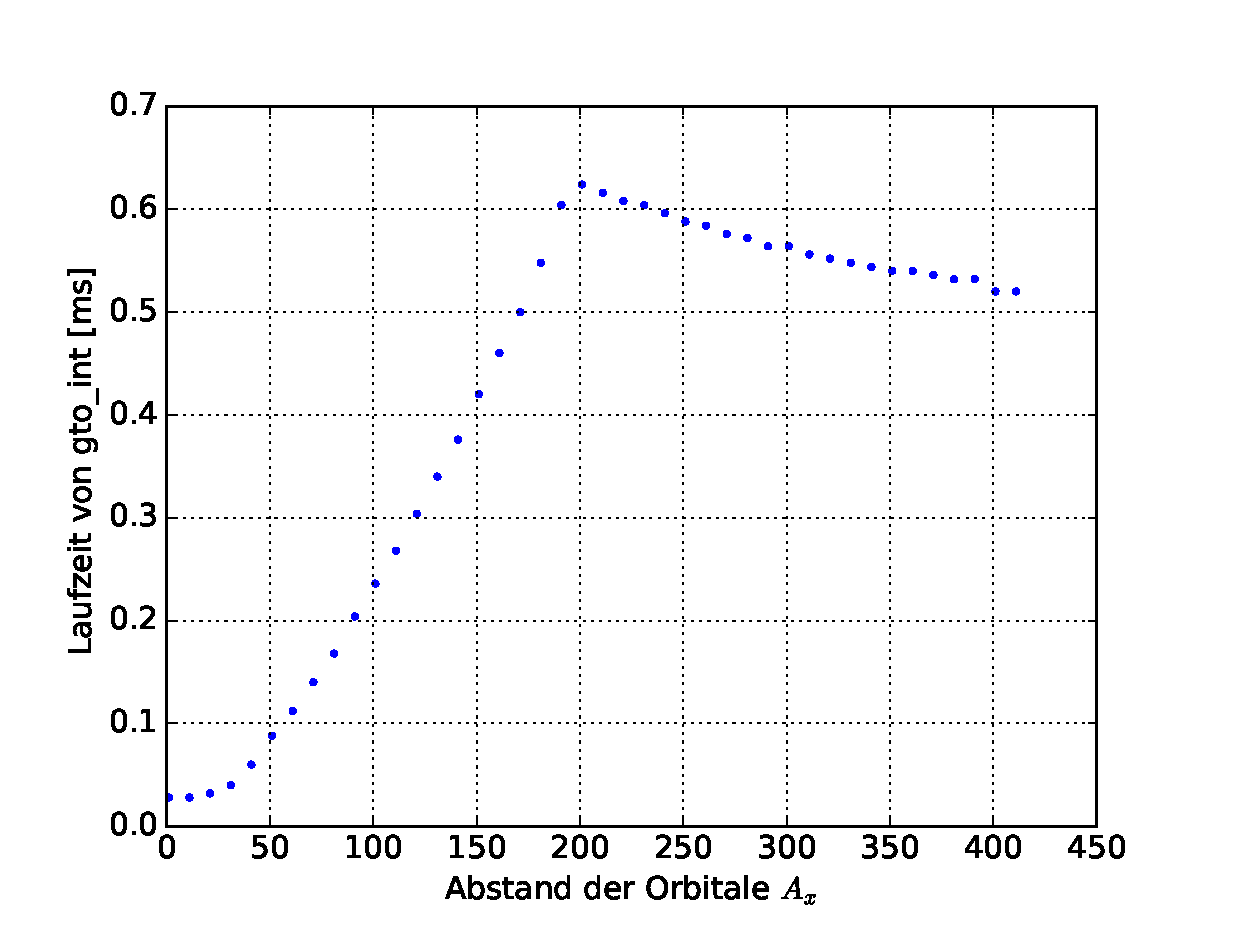
\includegraphics[scale=0.7]{Laufzeit_norm_abstand.eps}
	%\vspace*{-10mm}
	\caption{Laufzeit von \texttt{gto\_int} in Abhängigkeit des 
	Parameters $A_x$ bei der Normberechnung zu den 
	Orbitalen (0,0,1) und (0,0,0) und den Exponenten 
	a=c=0,001}
	%\vspace{2mm} %\hrule 
	\label{pic:test_norm_abstand_laufzeit} 
\end{figure}
%

%
%
%
\subsubsection{Variation des Exponenten}
%
Abschließend soll der Exponent a bzw. c variiert 
werden. Auch hier wird das (0,0,1) Orbital an 
\textbf{A}=($A_x$,0,0) in Verbindung mit dem an 
\textbf{C}=\textbf{0} 
befindlichen (0,0,0) Orbital betrachtet. Dazu muss 
zunächst ein plausibler Variationsbereich ermittelt 
werden. Das zu betrachtende physikalische Problem / 
System spielt auf zwei Größenordnungen an: zum einen auf 
der des Wechselwirkungspotentials und der des 
Fallenpotentials. Beide können in der Störungstheorie 
erster Ordnung um ihre Minima als quadratisch 
angenommen werden. Lösungen des Harmonischen Oszillators, 
Hermit-Funktionen, sind also in erster Ordnung eine 
gute Approximation der Wellenfunktionen. Dieser Sachverhalt ist in Bild 
\ref{pic:quad.naerung} dargestellt.
%
\begin{figure}[t] \centering
	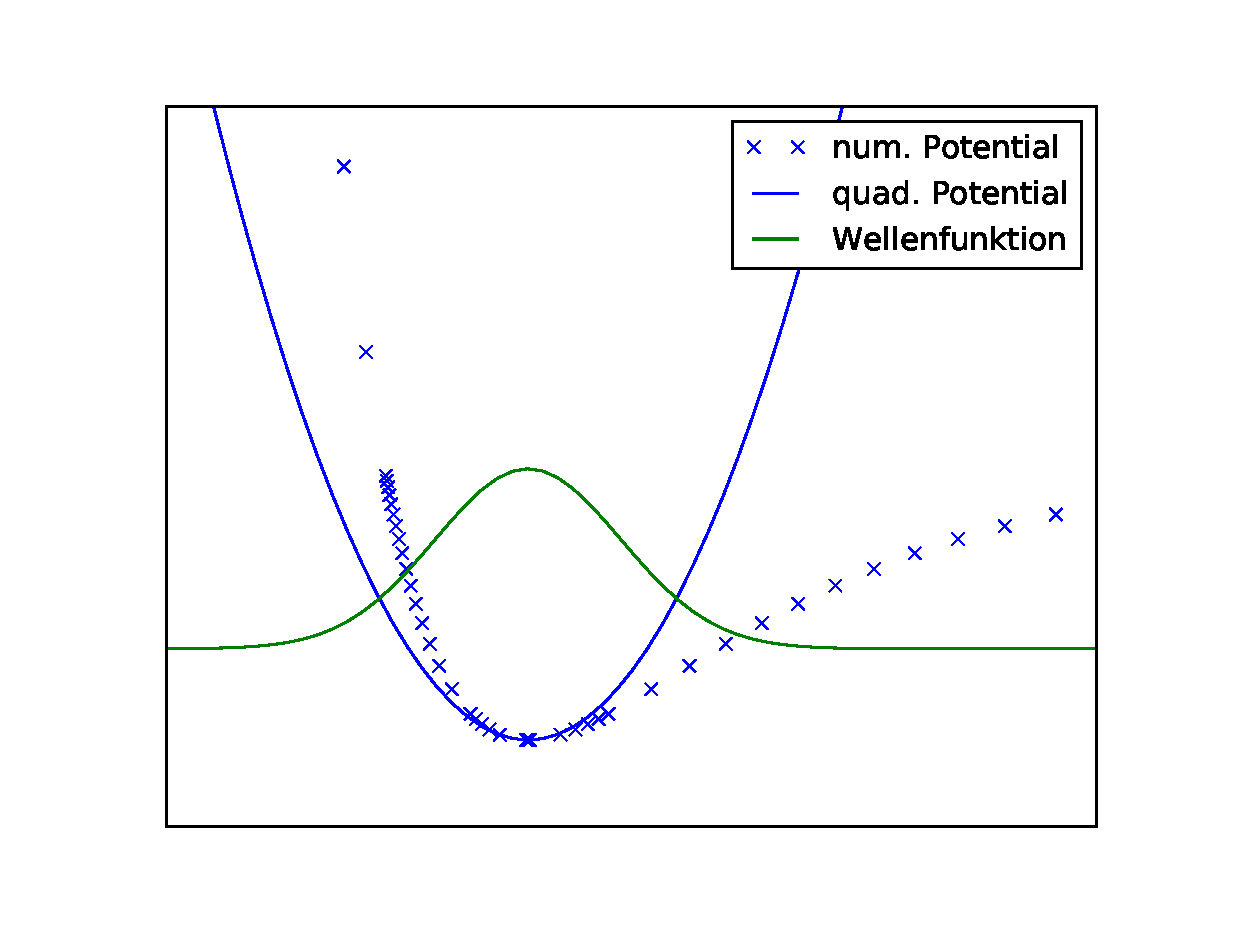
\includegraphics[scale=0.7]{HON.eps}
	\vspace*{-10mm}
	\caption{Schematische Darstellung der quadratischen Näherung und des 
	dazugehörigen Grundzustandes}
	%\vspace{2mm} %\hrule 
	\label{pic:quad.naerung} 
\end{figure}
%

Weiterhin macht diese Beobachtung zum einen die Wahl der GTOs als Ansatz sehr 
plausible, da die Hermit-(Gauß)-Funktionen in gewisser 
Weise enthalten sind und liefert auch eine Möglichkeit, 
um die Exponenten abzuschätzen. Der "Grundzustand"\ des 
als quadratisch genäherten Wechselwirkungspotentials 
kann analytisch berechnet werden. Das MRP \ref{eq:MRP} zum Beispiel nimmt in 
quadratischer 
Ordnung um das Minima\footnote{MRP stellt eine gute Beschreibung des 
numerischen Potentials um das Minima dar, vergleiche Darstellung 
\ref{pic:Pot}.} die Gestalt
%
\begin{align*}
V_\text{MRP}\approx-D_e + a_\text{st}^2\cdot D_e\cdot (r_{12}-R_m)^2 + 
\mathcal{O}(r_{12}^3) 
\end{align*}
%
an. Im Vergleich zum harmonischen Oszillator
%
\begin{align*}
V_\text{ham}=\frac12 m\omega_\text{h}^2 x^2
\end{align*}
% 
kann die Abschätzung
%
\begin{align*}
\frac12 m \omega_\text{h}^2 &= a_\text{st}^2 \cdot D_e\\
\Rightarrow \omega_\text{h}&=\sqrt{\frac{a_\text{st}^2\cdot D_e}{m}}
\end{align*}
%
gefunden werden. Aus dem Grundzustand des Harmonischen Oszillators 
%
\begin{align*}
\psi_0=\rl{\frac{m\omega_\text{h}}{\pi}}^\frac14 e^{-\frac12 m\omega_\text{h} 
x^2}
\end{align*}
%
kann nun der Exponent der Gauß-Funktion (Vergleiche \ref{pic:quad.naerung}), 
also der GTOs, 
unter Zuhilfenahme der Parameter aus Abbildung \ref{pic:Pot} und der 
Lithiummasse\footnote{$m_\text{Li}\approx12650,8 \ m_e$} in 
natürlichen Einheiten mit
%
\begin{align}
a_\text{max}\approx\frac{1}{2}a_\text{st}\sqrt{D_e\cdot m}\approx 1,074\  
a_0^{-2}
\end{align}
%
abgeschätzt werden.
Anschließend ist durch das Experiment \cite{av:7a} eine 
Frequenz für das Fallenpotential vorgegeben (siehe auch im Abschnitt 
\ref{sec:System}). 
\cite{phdthesis:sala} baut diesen Ansatz noch auf ein 
anharmonisches Potential aus, was hier noch nicht nötig 
ist. Es ergibt sich
%
\begin{align*}
a_\text{min}\approx\frac{m\omega_\text{exp}}{2}\approx2,142\cdot 10^{-9} \ 
a_0^{-2}\quad.
\end{align*}
%
Daher wird a bzw. c im Bereich von $1-10^{-10}$ 
variiert. 
%
\begin{table}[H] \centering
	\caption{Genauigkeitstest der Subroutine \texttt{gto\_int} 
		zu verschiedenen 
		Exponenten c der GTOs durch Normberechnung im Vergleich zu 
		analytischen 
		Ergebnissen mit den Konstanten a=0,001 und $A_x=1$} \vspace{0.2cm}
	\begin{threeparttable} 
		\begin{tabular}{c||c||c||c}
			c&$I_\text{gto\_int}$ & $I_\text{Norm}$ & 
			$\left|\frac{I_\text{gto\_int}-I_\text{Norm}}{I_\text{Norm}}\right|$
			 \\ \hline \hline
			1,00E+00 & 3,06407675221934E+07 & 3,06407675222225E+07 & 9,49E-13 \\
			1,00E-01 & 9,68946146259369E+08 & 9,68946146259369E+08 & 1,23E-16 \\
			1,00E-02 & 3,06407675222150E+10 & 3,06407675222225E+10 & 2,42E-13 \\
			1,00E-03 & 9,68946146260324E+11 & 9,68946146259369E+11 & 9,85E-13 \\
			1,00E-04 & 3,06407675221919E+13 & 3,06407675222225E+13 & 9,97E-13 \\
			1,00E-05 & 9,68946146259367E+14 & 9,68946146259369E+14 & 1,94E-15 \\
			1,00E-06 & 3,06407675224720E+16 & 3,06407675222225E+16 & 8,14E-12 \\
			1,00E-07 & 9,68946146163200E+17 & 9,68946146259369E+17 & 9,93E-11 \\
			1,00E-08 & 3,06407675140260E+19 & 3,06407675222225E+19 & 2,68E-10 \\
			1,00E-09 & 9,68946145997881E+20 & 9,68946146259369E+20 & 2,70E-10 \\
			1,00E-10 & 3,06407675222326E+22 & 3,06407675222225E+22 & 3,31E-13
		\end{tabular}
		%		\begin{tablenotes}
		%	\item[I] 
		%		\end{tablenotes}
	\end{threeparttable}
	\label{tab:norm:exp_c_A1}
\end{table}
%
In Tabelle \ref{tab:norm:exp_c_A1} ist zu sehen, dass das Programm über den 
gesamten Variationsbereich eine relative Abweichung von $10^{-10}$ nicht 
überschreitet. Eine leichte Tendenz zu schlechter werdenden Ergebnissen zu 
kleineren Exponenten, das heißt breiteren GTOs, ist zu erahnen. Nun soll der 
Exponent 
a variiert werden und c konstant gehalten 
werden. 
%
\begin{table}[H] \centering
	\caption{Genauigkeitstest der Subroutine \texttt{gto\_int} 
		zu verschiedenen 
		Exponenten a der GTOs durch Normberechnung im Vergleich zu 
		analytischen 
		Ergebnissen mit konstanten c=0,001 und $A_x=1$} \vspace{0.2cm}
	\begin{threeparttable} 
		\begin{tabular}{c||c||c||c}
			a&$I_\text{gto\_int}$ & $I_\text{Norm}$ & 
			$\left|\frac{I_\text{gto\_int}-I_\text{Norm}}{I_\text{Norm}}\right|$
			\\ \hline \hline
1,00E+00 & 3,06407675222224E+04 & 3,06407675222225E+04 & 2,37E-16 \\
1,00E-01 & 9,68946146259369E+06 & 9,68946146259369E+06 & 3,84E-16 \\
1,00E-02 & 3,06407675222217E+09 & 3,06407675222224E+09 & 2,30E-14 \\
1,00E-03 & 9,68946146260324E+11 & 9,68946146259369E+11 & 9,85E-13 \\
1,00E-04 & 3,06407675219172E+14 & 3,06407675222225E+14 & 9,96E-12 \\
1,00E-05 & 9,68946146259367E+16 & 9,68946146259369E+16 & 1,65E-15 \\
1,00E-06 & 3,06407677722220E+19 & 3,06407675222225E+19 & 8,16E-09 \\
1,00E-07 & 9,68945186259200E+21 & 9,68946146259369E+21 & 9,91E-07 \\
1,00E-08 & 3,06399483222180E+24 & 3,06407675222225E+24 & 2,67E-05 \\
1,00E-09 & 9,68684002260025E+26 & 9,68946146259369E+26 & 2,71E-04 \\
1,00E-10 & 3,06407675222326E+29 & 3,06407675222224E+29 & 3,32E-13 \\
1,00E-11 & 1,61319124067008E+32 & 9,68946146259369E+31 & 6,65E-01
		\end{tabular}
		%		\begin{tablenotes}
		%	\item[I] 
		%		\end{tablenotes}
	\end{threeparttable}
	\label{tab:norm:exp_a_A1}
\end{table}
%
In diesem Test ( Tabelle \ref{tab:norm:exp_a_A1} ) wird die schon oben 
beobachtete 
Tendenz zu schlechteren Ergebnissen zu kleineren Exponenten wieder beobachtet. 
Ein höheres Orbital, das heißt die höhere Komplexität, spiegelt sich damit auch 
in 
der Genauigkeit bei der Variation des Exponenten wider. Auffällig hier sind 
die Ergebnisse zu $a=\{10^{-5},10^{-10}\}$ . Hier scheinen sich numerische 
Fehler gegenseitig zu kompensieren. Weiterhin zeigt sich jetzt 
schon eine Grenzen des Programms. Für $a=10^{-11}$ fällt die Genauigkeit schon 
auf 66\% und ist damit wohl nicht mehr zweckdienlich. Dieser 
Genauigkeitsverlust entsteht vermutlich durch Verlust signifikanter Stellen bei 
einer Subtraktion zwei gleich großer Zahlen. Abschließend soll der 
letzte Test für einen anderen Abstand wiederholt werden:
 %
 \begin{table}[H] \centering
 	\caption{Genauigkeitstest der Subroutine \texttt{gto\_int} 
 		zu verschiedenen 
 		Exponenten a der GTOs durch Normberechnung im Vergleich zu 
 		analytischen 
 		Ergebnissen mit konstanten c=0,001 und $A_x=201$} \vspace{0.2cm}
 	\begin{threeparttable} 
 		\begin{tabular}{c||c||c||c}
 			a&$I_\text{gto\_int}$ & $I_\text{Norm}$ & 
 			$\left|\frac{I_\text{gto\_int}-I_\text{Norm}}{I_\text{Norm}}\right|$
 			\\ \hline \hline
1,00E+00 & 2,56024861643483E+04 & 3,06407675222225E+04 & 1,64E-01 \\
1,00E-01 & 8,24174537507960E+06 & 9,68946146259369E+06 & 1,49E-01 \\
1,00E-02 & 2,91305598288645E+09 & 3,06407675222224E+09 & 4,93E-02 \\
1,00E-03 & 9,68946146311261E+11 & 9,68946146259369E+11 & 5,36E-11 \\
1,00E-04 & 3,06407675222218E+14 & 3,06407675222225E+14 & 2,26E-14 \\
1,00E-05 & 9,68946146259371E+16 & 9,68946146259369E+16 & 1,98E-15 \\
1,00E-06 & 3,06407675222223E+19 & 3,06407675222225E+19 & 4,55E-15 \\
1,00E-07 & 9,68946146259313E+21 & 9,68946146259369E+21 & 5,80E-14 \\
1,00E-08 & 3,06407675221265E+24 & 3,06407675222225E+24 & 3,13E-12 \\
1,00E-09 & 9,68946146305179E+26 & 9,68946146259369E+26 & 4,73E-11 \\
1,00E-10 & 3,06407674635869E+29 & 3,06407675222224E+29 & 1,91E-09 \\
1,00E-11 & 9,68946146259346E+31 & 9,68946146259369E+31 & 2,40E-14 \\
1,00E-12 & 3,06407194882197E+34 & 3,06407675222225E+34 & 1,57E-06 \\
1,00E-13 & 9,68967117779157E+36 & 9,68946146259369E+36 & 2,16E-05
 		\end{tabular}
 		%		\begin{tablenotes}
 		%	\item[I] 
 		%		\end{tablenotes}
 	\end{threeparttable}
 	\label{tab:norm:exp_a_A201}
 \end{table}
 %
 Hier zeigt sich ein neuer Effekt. Für größere Abstände werden auch große 
 Exponenten ein Problem. Dieses Verhalten lässt sich wieder auf die Konvergenz 
 der 
 Reihendarstellung \ref{eq:reihe_M_kon.hyp.geo} zurückführen. An dieser 
 Stelle kann noch einmal auf die Größen \ref{eq:def:parameter y,x} hingewiesen 
 werden. y soll für eine gute Konvergenz in \ref{eq:reihe_M_kon.hyp.geo} 
 möglichst klein sein.  Ist a in der Größenordnung 1, geht y quadratisch mit 
 dem 
 Abstand. Für $A_x=201$ und a=1 ist $y\approx4\cdot10^4$, was definitiv nicht 
 mehr klein ist, wodurch das schlechte Ergebnis nicht mehr verwundert. Auf der 
 anderen Seite ist zu erkennen, dass ab a=$10^{-3}-10^{-4}$ das Ergebnis wieder 
 deutlich besser wird ($y\approx10-1$).\\
 
 Für die Tests \ref{tab:norm:exp_a_A1} und \ref{tab:norm:exp_c_A1} liegen die 
 Laufzeiten des Programms bei ungefähr 0,024 ms unabhängig vom Exponenten. Für 
 den letzten Test \ref{tab:norm:exp_a_A201} ist eine erhöhte Laufzeit für große 
 Exponenten mit 0,57 ms zu beobachten, was auf das Verhalten der 
 Reihenentwicklung zurückzuführen ist. Daraus folgert man außerdem, dass der 
 Genauigkeitsverlust für sehr kleine Exponenten nicht an der Reihendarstellung, 
 sondern an anderen Programmteilen liegt, wie oben schon vermutet.\\% 
 %Vorstellbar ist hier wieder der 
 %Verlust von signifikanten Stellen durch Subtraktion zweier Gleichgroßer 
 %Zahlen, wie z.B. in Formel \ref{eq:S,alpha>0}. \\
 
 Zusammenfassend kann gesagt werden, dass das Programm für niedrige Orbitale 
 und für kleine y, das heißt kleine Abstände und moderate Exponenten, eine 
 hinreichend gute relative Genauigkeit von mindestens $10^{-10}$ erreicht. Die 
 Laufzeiten sind für die gut zu bestimmbaren Integralen unter 1 ms und abhängig 
 vom Abstand noch deutlich geringer. 
%
%
%
\subsection{Reguläres Wechselwirkungspotential 
($f_{12}=r_{12}^2$)}\label{sec:T:quad}
%
Nachdem im letzten Abschnitt gezeigt wird, dass das Programm für ein neutrales 
Wechselwirkungspotential prinzipiell funktioniert, soll nun ein einfaches, 
nicht divergentes Wechselwirkungspotential getestet werden. Hier soll nun 
geprüft werden, ob das Programm auch mit einer Mischung der Koordinaten 
zurechtkommt und ob der Einfluss einer Wechselwirkung die Genauigkeit 
beeinflusst.  
Eine Problematik hierbei ist, dass nun das Integral nicht mehr mit Normen 
berechnet werden kann. Daher wird mit der numerischen Berechnung der 
NAG-Routine die Genauigkeit überprüft. \\
Auch hier sollen, um die Parameter übersichtlich zu halten, die Annahmen 
\ref{eq:tests:annahmen:norm} gelten.
Das Integral nimmt mit dem quadratischen Wechselwirkungspotential 
$f_{12}=V_2=r_{12}^2$
\ref{eq:def:V2} die Form
%
\begin{align*}
 I=\int\ d\textbf{r}_1 d\textbf{r}_2\   \cdot 
 x_{1,A}^{2i}\,y_{1,A}^{2k}\,z_{1,A}^{2m}\cdot e^{-2ar_{1,A}^2} \cdot r_{12}^2 
 \cdot x_{2,C}^{2i'}\,y_{2,C}^{2k'}\,z_{2,C}^{2m'} \cdot  e^{-2c 
 r_{2,C}^2}
\end{align*}
%
an. 
%
%
%
\subsubsection{Variation des Orbitals}
%
Zunächst wird analog zur Normberechnung die Abhängigkeit der Genauigkeit zur 
Wahl des Orbitals getestet. $(i',k',m')$ sei wieder $(0,0,0)$ und 
$(i,k,m)$ 
eine Variation.
%
 \begin{table}[H] \centering
 	\caption{Genauigkeitstest der Subroutine \texttt{gto\_int} 
 		zu verschiedenen 
 		Exponenten a der GTOs zu einem quadratischen Wechselwirkungspotential 
 		im Vergleich zu numerischen NAG-Routine mit konstanten c=0,001 und 
 		$A_x=1$} \vspace{0.2cm}
 	\begin{threeparttable} 
 		\begin{tabular}{c||c|c|c||c}
 Orbital & $I_\text{gto\_int}$ & $I_\text{NAG}$& ACC [\%] & 	
 $\left|\frac{I_\text{gto\_int}-I_\text{NAG}}{I_\text{gto\_int}}\right|$
 \\ \hline\hline
(0,0,0)&3,87578458503748E+09 & 3,8757822000E+09 & 6,73E-05 & 6,15E-07 \\
(0,0,1)&9,68946146259370E+11 & 9,6893670144E+11 & 1,02E-04 & 9,75E-06 \\
(0,0,2)&7,26709609873341E+14 & 7,2670802178E+14 & 9,03E-05 & 2,19E-06 \\
(1,0,0)&9,68946146260324E+11 & 9,6894050977E+11 & 1,07E-04 & 5,82E-06 \\
(1,0,1)&2,42236536624686E+14 & 2,4223431793E+14 & 1,71E-04 & 9,16E-06 \\
(1,2,0)&1,81677760185790E+17 & 1,8167479946E+17 & 1,44E-04 & 1,63E-05 \\
(2,0,0)&7,26709611782121E+14 & 7,2642851744E+14 & 8,18E-05 & 3,87E-04 \\
(2,0,1)&1,81678118290674E+17 & 1,8137431973E+17 & 1,28E-04 & 1,67E-03
 		\end{tabular}
 		%		\begin{tablenotes}
 		%	\item[I] 
 		%		\end{tablenotes}
 	\end{threeparttable}
 	\label{tab:r2_orbit}
 \end{table}
%
Wie in Tabelle \ref{tab:r2_orbit} zu sehen, liefert \texttt{gto\_int} 
vergleichbare, 
wahrscheinlich bessere Ergebnisse als die NAG-Routine für kleine Orbitale. Die 
wahre Genauigkeit kann hier nicht abgeschätzt werden, da die NAG-Routine auf 
ungefähr $10^{-4}-10^{-5}$ beschränkt ist. Im Vergleich zur Normberechnung 
stellt man 
jedoch fest, dass schon das (2,0,1) Orbital deutlich schlechter geworden ist. 
Weiterhin stellt man fest, dass das Integral des (2,0,0) Orbitals wesentlich 
schlechter als das Integral des (0,0,2) Orbitals berechnet wird. Anscheinend 
ist also die Genauigkeit durch die Potenz in Richtung des Abstandes  
beeinflusst und nun nicht mehr für alle Orbitale des selben l gleich. %TODO 
%LAUFZEIT fatzit 
%
%
%
\subsubsection{Variation des Abstands}
%
Nun soll der Abstandsparameter $A_x$ variiert werden. Grafik 
\ref{pic:quad.WW_Abstand} zeigt die Integralwerte der \texttt{gto\_int} Routine 
im 
Vergleich zur NAG-Routine und einer quadratischen Funktion.
%
\begin{figure}[H] \centering
	\subfigure[]{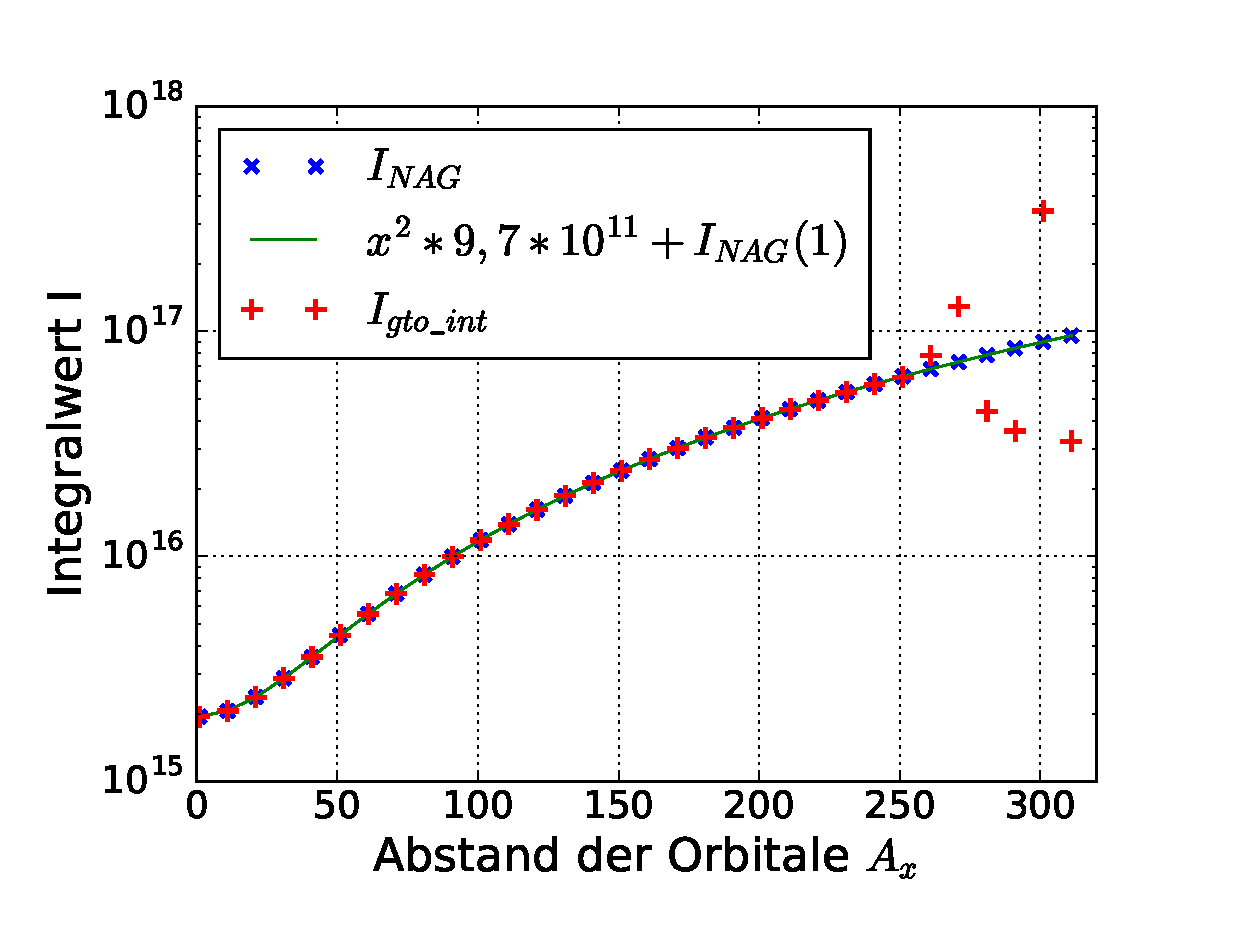
\includegraphics[scale=0.55]{r2_1.eps}} %0.35
	\subfigure[]{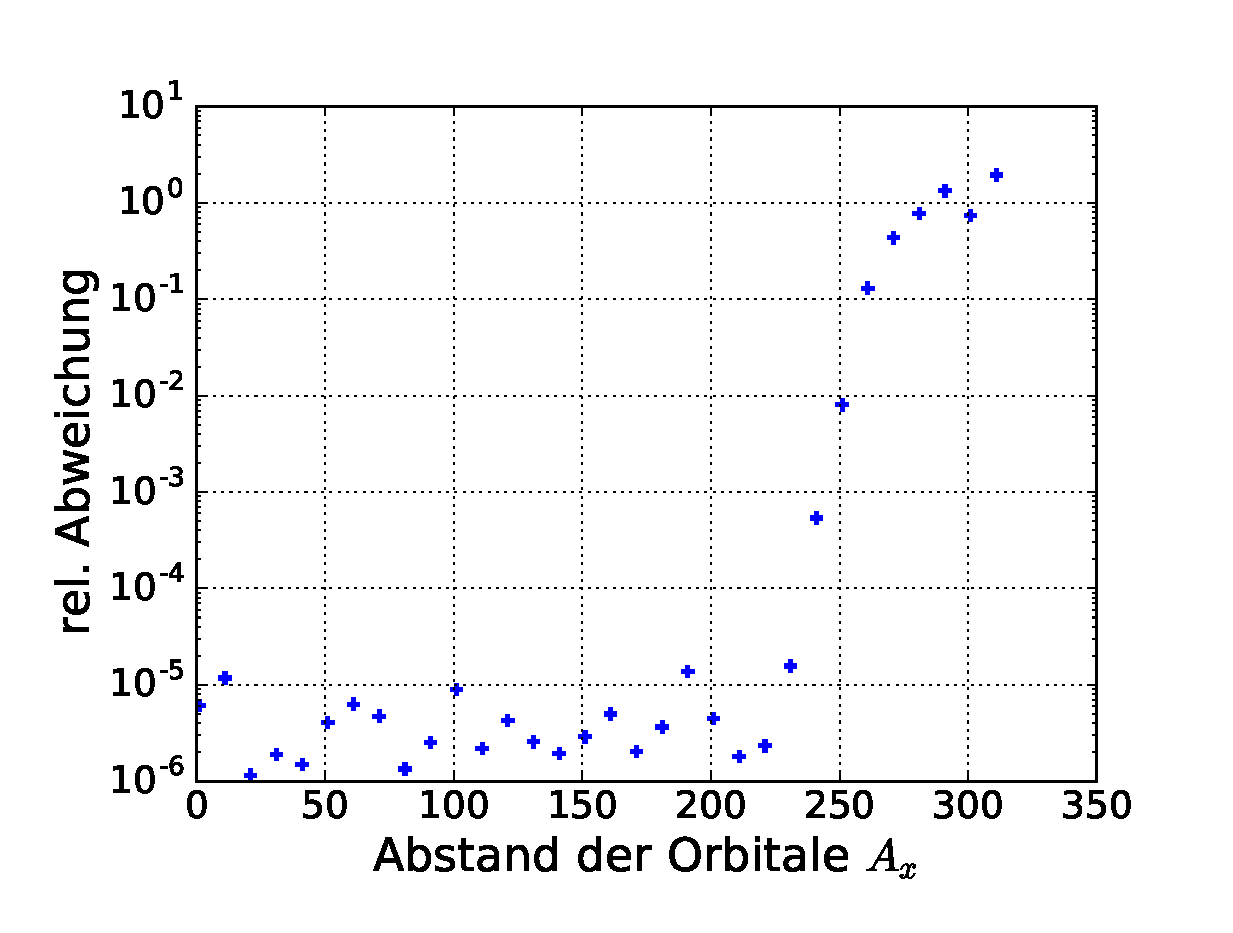
\includegraphics[scale=0.55]{r2_2.eps}}
	%\vspace*{-10mm}
	\caption{(a) Vergleich der Ergebnisse der \texttt{gto\_int} und der 
	NAG-Routine zu 
	verschiedenen Werten des Abstandsparameters $A_x$, wobei die Orbitale 
	(1,0,0) mit dem Exponenten a=0,001 und (0,0,0) mit dem Exponenten c=0,001 
	betrachtet worden sind. 	Zusätzlich ist eine quadratische Funktion 
	dargestellt. 
	(b)  zeigt die relative Abweichung zwischen $I_\text{NAG}$ und 
	$I_\text{gto\_int}$ .  } 
	%\vspace{2mm} %\hrule 
	\label{pic:quad.WW_Abstand}
\end{figure}
%
Vergleichbar zum analogen Test bei der Normberechnung sieht man in Grafik 
\ref{pic:quad.WW_Abstand} (b) , dass \texttt{gto\_int} für $A_x$ größer als 
rund 
230 einen immer größer werdenden Genauigkeitsverlust hat. Vergleicht man mit 
der 
Tabelle \ref{tab:norm:abstand_2} im Anhang \ref{sec:AnhangC:Tests}, so kann  
festgestellt werden, dass auch dort für $A_x$ größer als 230 die Genauigkeit 
schlechter als $10^{-5}$ wird. Daher scheinen für die Variation des Abstandes 
eines gegebenen Orbitals, keine neuen Verluste aufzutreten. Der rapide 
Genauigkeitsverlust kann analog zur Normberechnung auf die Reihendarstellung 
\ref{eq:reihe_M_kon.hyp.geo} zurückgeführt werden. Die Laufzeit hat auch die in 
Grafik \ref{pic:test_norm_abstand_laufzeit} dargestellten Verlauf und befindet 
sich in der selben Größenordnung. \\
In Abbildung \ref{pic:quad.WW_Abstand} (a) ist zu erkennen, dass 
$I_\text{gto\_int}$ den numerischen Ergebnissen $I_\text{NAG}$ weitgehend 
folgt. Zusätzlich kann man feststellen, dass bei Verwendung einer quadratischen 
Wechselwirkung die Integralwerte entsprechend eines quadratischen Verlaufs bei 
der Variation des Abstandes zeigen, was durch die hinzugefügte Funktion 
ersichtlich ist. Die Integralwerte fächern bei steigender Ungenauigkeit um das 
richtige Ergebnis auf.    
%
%
%
\subsubsection{Variation des Exponenten}
%
Bei der Variation des Exponenten ist analog zur Normberechnung vorgegangen 
worden, das heißt, die Tests werden unter den gleichen Annahmen und mit den 
selben 
Werten der konstanten Parameter durchgeführt. Dabei ist ein immer gleiches 
Verhalten beobachtet worden. 
%
\begin{figure}[H] \centering
	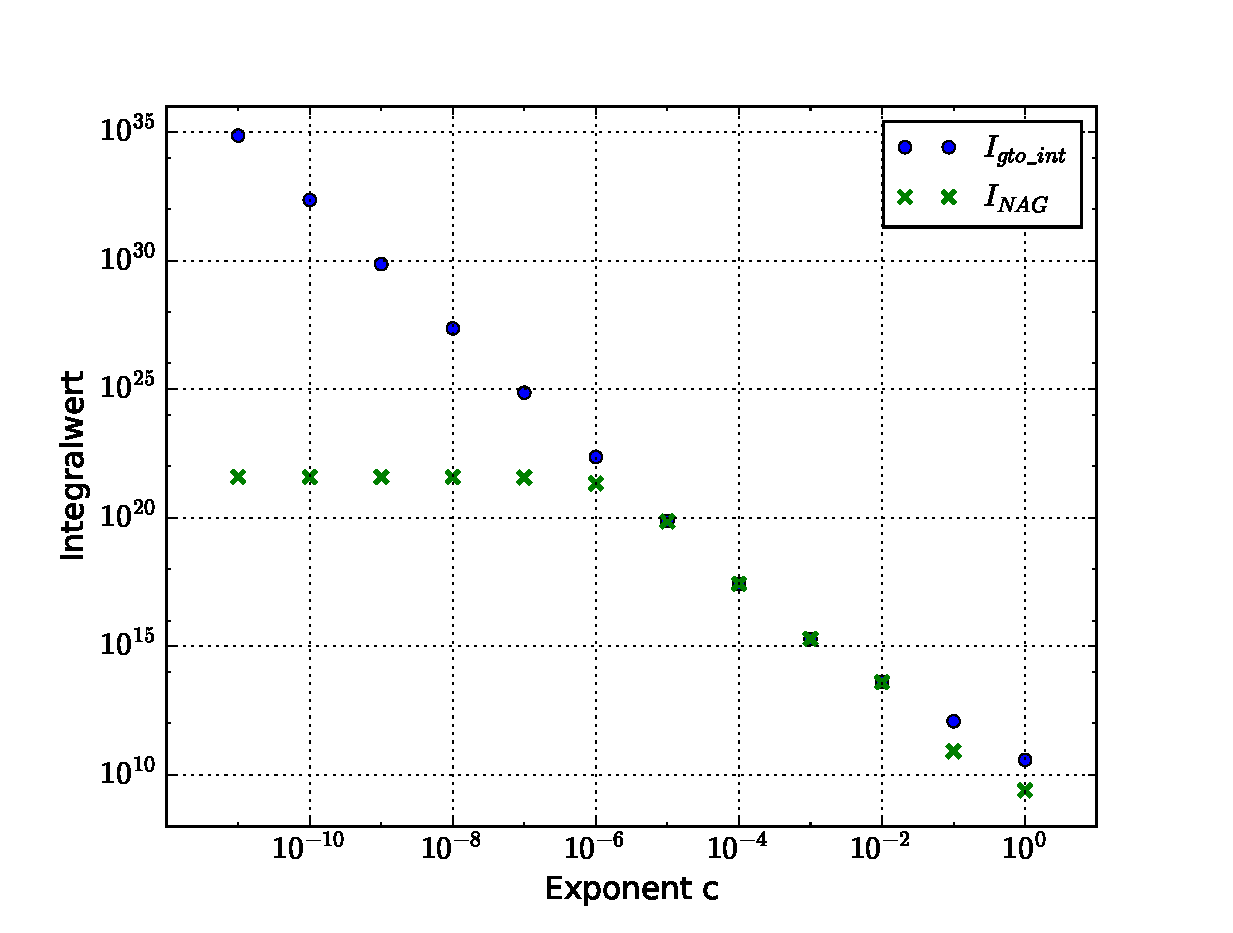
\includegraphics[scale=0.7]{r2_3.eps}
	%\vspace*{-10mm}
	\caption{Vergleich der Ergebnisse der \texttt{gto\_int} und der NAG-Routine 
	zu unterschiedlichen Exponenten c bei a=0,001 , $A_x=101$ und 
	\textbf{C}=\textbf{0}.}
	%\vspace{2mm} %\hrule 
	\label{pic:quad.WW_exponent} 
\end{figure}
%
Wie in Abbildung \ref{pic:quad.WW_exponent} zu sehen ist, gibt es zwei Bereiche,
in denen \texttt{gto\_int} von der NAG-Routine abweicht und einen Bereich 
($10^{-2}-10^{-5}$), indem sie folgt. Im Letzteren beträgt die Abweichung 
ungefähr $10^{-6}$; wie oben schon gesehen, stimmt in dem Bereich also 
\texttt{gto\_int} so gut es nur geht mit $I_\text{NAG}$ überein. Für große 
Exponenten tritt wieder die oben beschriebene Abweichung aufgrund der 
Reihendarstellung im Basisintegral ein. Die auftretende Abweichung für 
Exponenten kleiner als $10^{-5}$ ist ein technisches Problem. Bei der 
Verwendung der NAG-Routine muss ein endliches Berechnungsintervall gegeben 
werden. Da für kleine Exponenten die GTOs aber immer breiter werden, wird 
irgendwann das gesamte Intervall von der GTO ausgefüllt und es wird quasi über 
eine Waagerechte integriert (Rechteck). Daher nimmt $I_\text{NAG}$ einen 
maximalen Wert an für kleiner werdende Exponenten. Es wird versucht, 
entsprechend das Intervall auf eine andere Größenordnung mit zu skalieren, 
jedoch scheint die NAG-Routine intern Abtastalgorithmen zu verwenden, die dann 
keine veränderliche Funktion mehr wahrnimmt, frühzeitig abbricht und 0 als 
Ergebnis ausgibt. Analog sei erwähnt, dass auch die Abweichung für große 
Exponenten prinzipiell durch Fehler beim Abtasten in der NAG-Routine 
entstanden sein kann.   %\\%letztes ist seh wichtig !!
Weiterhin ist in \ref{pic:quad.WW_exponent} zu erkennen, dass der prinzipielle 
Verlauf der Integralwerte von $I_\text{NAG}$ im Übereinstimmungsbereich weiter 
gefolgt wird. Das ist ein Indiz dafür, dass  $I_\text{gto\_int}$ auch für 
kleinere Exponenten plausible Werte liefert. Hinzu kommt, dass auch noch kein 
Auffächern oder ähnliche extreme Schwankungen zu erkennen sind.
%
%
%
\subsection{Renormierungsschema}
%
In \texttt{int\_S\_sub} wird innerhalb der T-Blöcke ein Renormierunsschema 
verwendet. Dieses ist im Abschnitt \ref{sec:renorm} erklärt. Auf Grund der 
Renormierung können solche Integrale nicht mit einer numerischen Routine 
überprüft werden. Daher wird die Untersuchung der Plausibilität der 
Integralwerte nicht mehr in dieser Arbeit erörtert. Die Lösung (das 
Energiespektrum) für das 
Zweiteilchenproblem $^7$Li$^7$Li ist in \cite{phdthesis:sergey} gegeben, 
daher kann das Renormierungsschema an diesem physikalischen Beispiel getestet 
und geprüft werden, was auch nicht mehr in dieser Arbeit geschieht. Im Vorfeld 
kann jedoch noch eine Konsistenzprüfung durchgeführt werden. Zur Erinnerung es 
geht um Integrale des Typs \ref{eq:def:T-Int} :
%
\begin{align*}
T_s^\pm(x)&:=\mathcal{R}\int_{0}^{\infty}\frac{dz}{z^s}e^{\pm z-xz^2} \quad.
\end{align*}
%
Zur Berechnung dieser ist im Abschnitt \ref{sec:renorm} erklärt, dass die 
Rekursion \ref{eq:recursivT} für $x=\frac{\gamma}{\beta^2}>1$ und die Rekursion 
\ref{recursiveT2} für x<1 verwendet werden soll, wobei $\gamma$ und 
$\beta$ potentialspezifische Parameter sind.  \ref{eq:recursivT} 
 startet mit berechenbaren Integralen. $\omega_1(x)$ und $\omega_0(x)$ sind 
 durch numerische Integration im Rahmen der in \cite{av:1a2} angegebenen 
 Grenzen überprüft worden. Auf Tipp- und Logikfehler ist durch eine unabhängige 
 MATHEMATICA-Implementierung getestet worden. Dabei sind für \ref{eq:recursivT} 
 keine Anomalien aufgetreten. Bei der Berechnung der Rekursion 
 \ref{recursiveT2} (fallender Index) hingegen ist aufgefallen, dass $T_s$ nicht 
 unabhängig von dem gewählten oberen Startindex $s_\text{max}$ ist. Abbildung 
 \ref{pic:Trec} zeigt das Verhalten an 3 repräsentativen Beispielen für 
 verschiedene x.    
%
\begin{figure}[t] \centering
	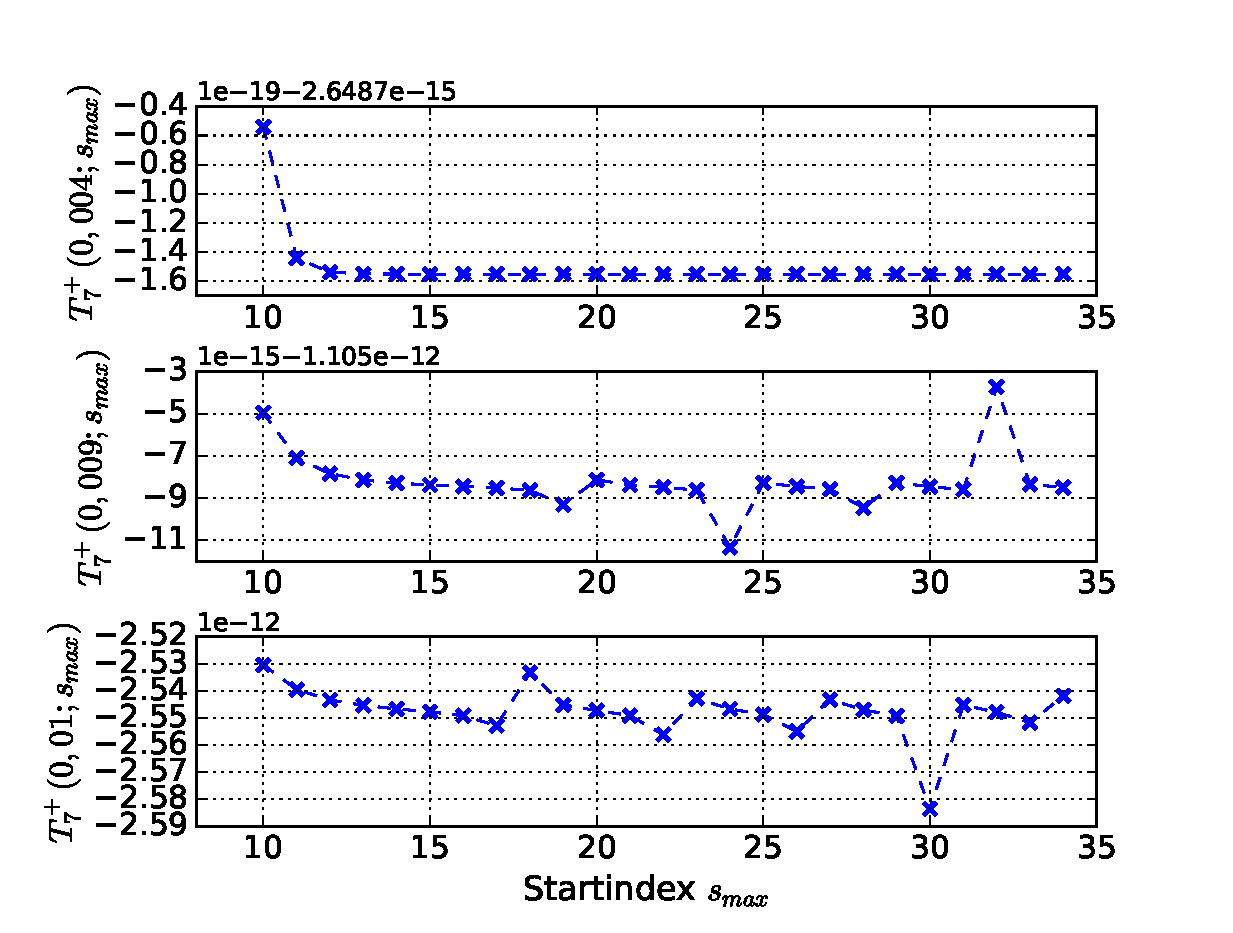
\includegraphics[scale=0.7]{Trec.eps}
	%\vspace*{-10mm}
	\caption{Konvergenzverhalten der Rekursion \ref{recursiveT2} zur Berechnung 
	von $T^+_s(x)$ für 
	verschiedene Startindizes $s_\text{max}$ am Beispiel s=7 und x=$\{0,004 ,\ 
	0,009 ,\ 0,01 \}$ }
	%\vspace{2mm} %\hrule 
	\label{pic:Trec} 
\end{figure}
%

Zu erwarten wäre ein Annähern der Integralwerte an eine 
Konstante, sodass es ein fixes $s_\text{max}$ gibt, ab dem die Rekursion 
unabhängig von $s_\text{max}$ wird. 
Zunächst ist zu sagen, dass die FORTRAN Implementierung bei x<0,004 als 
Ergebnis 0 ausgibt. Zumal kann $T_0^+$ hier schon auf Grund des 
Exponentialfaktors $e^{\frac{1}{4x}}$ den Darstellungsbereich 
\texttt{real(KIND=8)} (double percision) verlassen und so bei der 
Nachskalierung einen undefinierten Wert ergeben. Weiterhin kann es dazu kommen, 
dass z.B. $T_0^-$ auf exakt 0 gerundet wird, da die \texttt{Erf}-Funktion schon 
auf exakt 1 gerundet wird. \\
Im obersten Bild der Grafik \ref{pic:Trec} ist zu erkennen, dass hier das 
beschriebene Vorgehen aus Abschnitt \ref{sec:renorm} äußerst gut funktioniert. 
Es wird ab $s_\text{max}=28$ ein auf 16 signifikante Stellen konstantes 
Ergebnis berechnet\footnote{Alle Berechnungen sind bis $s_\text{max}=100$ 
durchgeführt worden, jedoch nur bis $s_\text{max}=34$ dargestellt.}. Im 
mittleren und unteren Bild ist jedoch zu erkennen, dass die Rekursion abhängig 
von $s_\text{max}$ nicht auf die gewünschte Genauigkeit konvergiert. Für kleine 
Startindizes ist das erwartete Annähern an das Ergebnis zu beobachten, jedoch 
schlägt z.B. im mittleren Bild bei $s_\text{max}=19$ die Kurve aus. 
Anschließend scheint wieder eine Annäherung zu entstehen, welche durch einen 
weiteren Ausschlag bei 24 unterbrochen wird. Die Schwankungen liegen im 
mittleren Bild im Bereich von 0,1\%. Ein analoges Verhalten ist auch in 
untersten Bild in \ref{pic:Trec} zu sehen. Hier liegt die Schwankung jedoch in 
Bereich von 10\%. Die Tendenz, dass pro 0,001 Schritt in x 2-3 Größenordnungen 
der Genauigkeit verloren geht, ist auch für 0,004<x<0,009 und für x>0,01 zu 
sehen. Im letzteren Fall hat man also keine signifikanten Stellen des 
Ergebnisses mehr, lediglich eine Größenordnung. Für größere x sind die 
Sprungstellen und die abschnittsweise Annäherung an das Ergebnis, analog zur 
Abbildung \ref{pic:Trec}, deutlicher zu sehen.  Es stellt sich nun die Frage ob 
die Verwendung in einem so eingeschränkten Anwendungsbereich noch Sinn macht. 
Um die Genauigkeit zu verbessern, kann versucht werden die Rekursion 
\ref{recursiveT2} auf einem höheren Datentyp (z.B. \texttt{real(KIND=16)}) 
ablaufen zu lassen, da Verlust signifikante Stellen durch Subtraktion zweier 
gleich großer Zahlen entstehen kann.
%
%
%
%\subsection{Zusammenfassung}
%
%Im Rahmen der hier dargestellten Tests ist festgestellt worden, dass 
%\texttt{gto\_int} für niedrige Orbitale, das heißt l<6 ,effektive Abstände 
%Q<200 und für große Bereiche der Exponenten a/c eine relative Genauigkeit von 
%ungefähr $10^{-10}$ erreichen kann. Der limitierende Faktor bzgl. des 
%Abstandes 
%stellt die Reihendarstellung \ref{eq:reihe_M_kon.hyp.geo} und damit die 
%Berechnung des Basisintegrals dar. Die Größe y sollte dabei möglichst kleiner 
%als 1 sein. Für höhere Orbitale und Exponenten kleiner als $10^{-10}$ sind 
%andere Effekte verantwortlich. Zu vermuten ist, dass bei einer Subtraktion 
%zweier gleichgroßer Zahlen signifikante Stellen verloren gehen.
% 
%
%
\section{Optimierungsvorschläge}
%
In diesem Projekt wird in erster Linie darauf hin gearbeitet, das Programm 
\texttt{gto\_int} bzw. \texttt{gto\_int\_test} und damit den Algorithmus zum 
Laufen zu bringen. Hierbei wird aus Zeitgründen und der Einfachheit halber 
einige Kompromisse bzgl. der Programmoptimierung getroffen. Im Folgenden werden 
schon bekannte, aber noch nicht implementierte Optimierungen des Quellcodes 
vorgeschlagen.
\begin{enumerate}
	\item Es soll eine andere Berechnungsmethode des Basisintegrals 
	gefunden und implementiert werden. Dazu bietet sich an, den in 
	\cite{av:1a} / \cite{av:1a2} vorgestellten Weg zu wählen, jedoch muss 
	dazu 
	erst der Fehler in Gleichung (60) aus \cite{av:1a} berichtigt und auf 
	alle darauf folgenden Gleichungen angewandt werden, erste Ansätze sind 
	dafür schon vorhanden.
	%
	\item Im Programmabschnitt \texttt{sum\_R\_sum} werden die soliden reellen 
	Kugelflächenfunktionen Z als Funktion von sin und cos Funktionen 
	aufgerufen. Da der Vektor \textbf{Q} und damit deren Polardarstellung schon 
	kurz nach Aufruf der \texttt{gto\_int} Routine bekannt ist, soll schon dort 
	der sin und cos Wert ausgewertet und gespeichert werden. So kann eine 
	ganze Reihe an Funktionsaufrufen, die in Reihenentwicklungen enden, 
	eingespart werden. Weiterhin kann so Z schon als Matrix oder besser Vektor 
	vor den äußeren Schleifen in \ref{pic:FC:sum_R_sub} berechnet werden; dies 
	spart wiederum Laufzeit und Speicherplatz.
	%
	\item Der Koeffizient $c^{-1}$ in \texttt{sum\_R\_sub} wird über Aufrufe 
	der Schlegel-Koeffizienten c berechnet. Dabei wird aktuell c noch als 
	Funktion gehandhabt. Sowohl c als auch $c^{-1}$ können, da sie von keinen 
	fallspezifischen Parametern abhängen, einmalig für einen großen Bereich 
	der Indizes, berechnet und auf der Festplatte gespeichert werden. Dabei 
	soll weiterhin eine Vektorisierung des noch 5-d-Feldes vorgenommen werden. 
	Diese Optimierung 	spart Rechenzeit, da weniger Funktionsaufrufe und 
	keine Berechnungsschleifen mehr notwendig sind. Weiterhin spart man dabei 
	Speicherplatz, da durch eine Vektorisierung keine nicht genutzten Nullen 
	mehr gespeichert werden müssten.
	%
	\item Der Koeffizient d in \texttt{sum\_R\_sub} wird innerhalb von einer 
	Schleife berechnet, das heißt, \texttt{d\_coef} wird dort erst aufgerufen. 
	Es soll \texttt{d\_coef} so	angepasst werden, sodass der Aufruf schon 
	außerhalb der Schleife geschehen kann. Weiterhin  ist d auch unabhängig von 
	fallspezifischen Parametern, das heißt,	auch d kann einmal vorberechnet 
	und anschließend auf der Festplatte gespeichert werden. Diese 
	können dann für alle folgenden Integrale abgerufen werden. Außerdem soll 
	auch d als Vektor gespeichert werden, um die Laufzeit weiter zu optimieren 
	und unnötige Nullen nicht zu speichern.
    % 
\end{enumerate} 
%
%
%
%\chapter{Zusammenfassung}

Es ist der Algorithmus zur Berechnung von sechsdimensionalen 
Wechselwirkungsintegralen, präsentiert in \cite{av:1a} für 
Elektronenstrukturrechnungen, überprüft, zum Teil berichtigt 
und an ein System von zwei ultrakalten Atomen angepasst 
worden. Zwei Näherungsfunktionen für realistische 
Wechselwirkungspotentiale sind vorgestellt und die Anwendung 
des Algorithmus, das heißt die Berechnung der Basisintegrale 
unter Benutzung der Näherungsfunktionen, ist analytisch 
vorbereitet worden. \\
Der Algorithmus ist in der Programmiersprache FORTRAN als 
Subroutine \texttt{gto\_int} implementiert und getestet 
worden. Dabei kann gezeigt werden, dass \texttt{gto\_int} für 
reguläre Potentiale, das heißt Integrale, die nicht renomiert 
werden müssen, in einem gewissen Parameterbereich präzise 
Ergebnisse liefert. Bei Anwendung des Renormierungsschemas 
zeigt sich jedoch ein  eingeschränkter Anwendungsbereich, 
falls x<1 ist. 
Weiterhin sind Vorschläge zur Optimierung des 
Programms angebracht worden.\\

Der unmittelbar nächste Schritt sollte es sein, das hier 
beschriebene Programm 
im Rahmen einer CI Rechnung auf das echte physikalische 
System mithilfe des nicht zu renomierenden Morse-Potentials 
anzuwenden und zu testen ob ein mit \cite{phdthesis:sergey} 
vergleichbares Energiespektrum berechenbar ist. Falls dabei 
festgestellt werden sollte, dass der 
Anwendungsbereich aktuell nicht groß genug ist, dann sollten  
relevante Optimierungen umgesetzt und erneut getestet werden. 
Weiterhin ist noch nicht geklärt, inwiefern das 
Renormierungsschema bei Verwendung des 
Lennard-Jones-Potentials konvergiert und ob damit eventuell 
ein vergleichbares, besseres oder schlechteres Ergebnis 
erzielt werden kann. Überprüft werden sollte dies, da das LJP 
prinzipiell die physikalische Gegebenheit für größere 
Abstände der Atome besser beschreibt. 
Weiterhin lässt \texttt{gto\_int} im Rahmen einer CI Rechnung 
auch mehr als nur 2 
Teilchen / Atome zu. Daher kann, falls das Zweiteilchensystem 
zu plausiblen Ergebnissen kommt, das Programm auf größere 
Systeme angewandt werden. 

%kann gezeigt werden
%zeigt sich
% \chapter{Theorie}
%
%
%\section{Theoretische Grundlagen}
%
Im Rahmen dieser Arbeit werden, wenn nicht anders gekennzeichnet, atomare
Einheiten verwendet. Das bedeutet, Energien werden in Einheiten von \\ 1 $E_h$ 
(Hartree) =  2 Rydberg $\approx$ 27.21 eV, Massen in 1 $m_e$, Strecken in 1
$a_0$ und Ladungen in Einheiten von 1 $e$ angegeben.
%
%
%
\section{System}\label{sec:System}
%
Untersucht wird ein ultrakaltes Zweiteilchensystem.
Stellvertretend für andere Systeme kann das bosonische Zweiatomsystem 
Li$^7$Li$^7$ betrachtet werden. Der Hamilton-Operator 
%
\begin{align}\label{eq:kernHam1}
	\Op{H}=\sum_{i=1}^{2}\Op{T}_{K_i}
		+\sum_{i=1}^{2} \Op{V}_{\text{F}}(\textbf{r}_i)
		+\Op{U}(|\textbf{r}_1-\textbf{r}_2|) 
\end{align} 
% 
beschreibt mithilfe der nicht-relativistischen, stationären Schrödingergleichung
%
\begin{align}\label{eq:algSg1}
	\Op{H}\Ket{\psi} = \text{E} \Ket{\psi}
\end{align}
%
das System. 
$\Op{T}_{K_j}=\frac{1}{2\text{M}}\nabla^2_{r_j}$\
ist der 
Kinetische-Energieoperator des jeweiligen Kerns. $\Op{V}_\text{F}$ beschreibt 
ein
Fallenpotential, welches in dieser Arbeit als isotrop und harmonisch angenommen 
wird, das 
heißt 
%
\begin{align}
\Op{V}_\text{F}(\text{r}_i) = \frac{1}{2}\,\text{M}\,\omega^2\, 
\textbf{r}^2_i=\frac{1}{2}\,\text{M}\,\omega^2 \rl{ \, \text{x}^2_i + 
\text{y}^2_i + 
\text{z}^2_i\, } \quad.
\end{align}
%. 
$\Op{U}$  ist eine aus 
Elektronenstrukturrechnung oder Experimenten bekanntes oder motiviertes  
effektives Wechselwirkungspotential. Für Li$^7$Li$^7$ ist in 
\cite{phdthesis:sergey} und den darin enthaltenden Referenzen ein 
solches Potential stückweise zusammengestellt worden, das 
in Grafik 
\ref{pic:NP} dargestellt ist. \\
 
%
%\begin{figure}[t] \centering
%	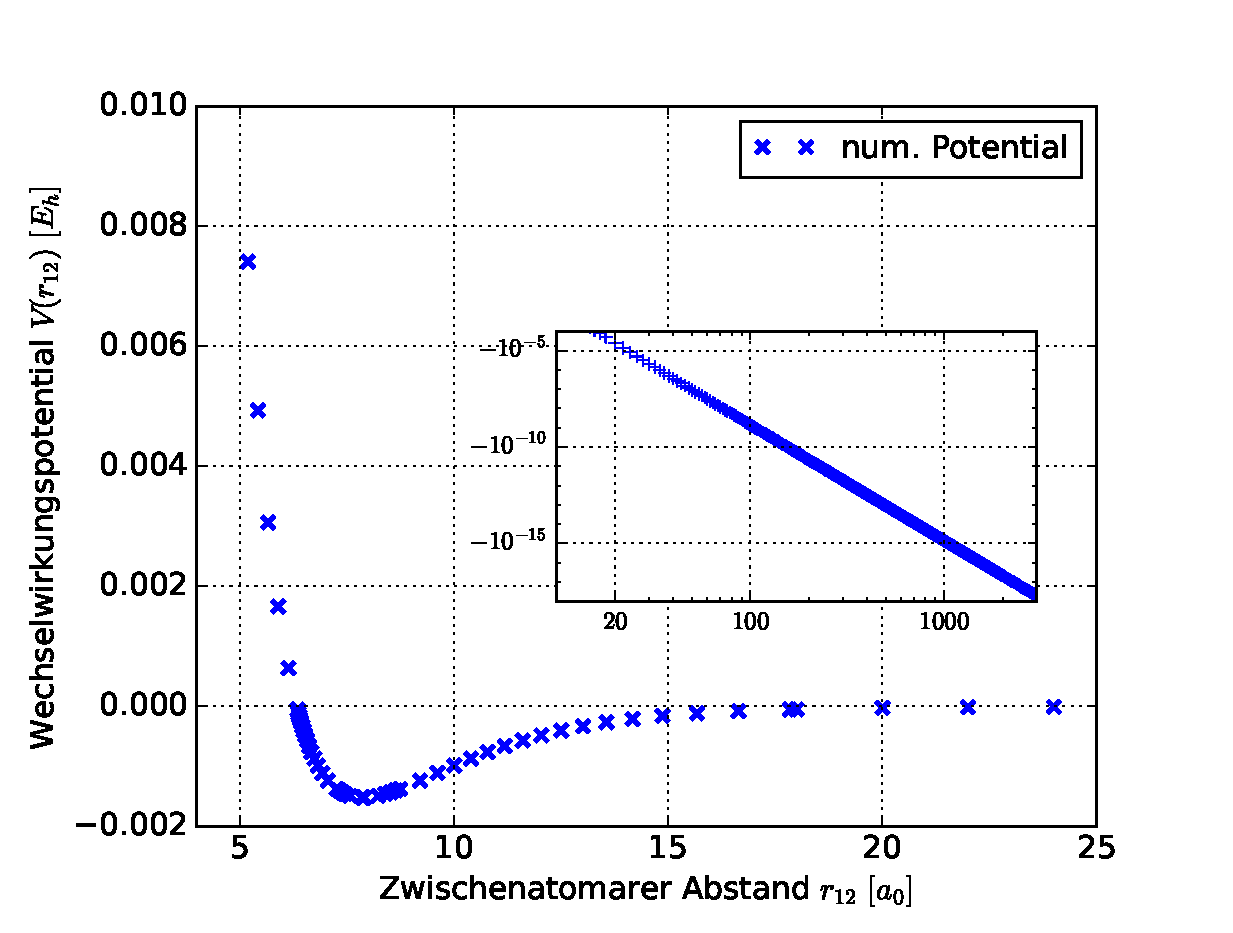
\includegraphics[scale=0.65]{NP.eps}
%	%	\vspace*{-10mm}
%	\caption{Dargestellt ist ein numerisches 
%	Wechselwirkungspotential (gekreuzt) eines 
%		angeregten Tripletzustandes des 
%		$^7$Li$^7$Li Systems.}
%	%\vspace{2mm} %\hrule 
%	\label{pic:NP} 
%\end{figure}
%
Eine mögliche experimentelle Vorlage für ein Zweiatomsystem ist 2011  
realisiert worden \cite{av:7a}.
 Hier handelt es sich um eine
optische Dipolfalle, welche in erster Ordnung auch durch ein quadratisches
Potential beschrieben werden kann  \cite{phdthesis:sala}.  Die ermittelte 
effektive Fallenfrequenz liegt in der Größenordnung von
$10^{4}$ Hz $\approx$ $10^{-13}\ \omega_0$ in atomaren Einheiten. 
% 
\pagebreak
%
%
%
\section{Konfigurationswechselwirkungsrechnung}
%
Da \ref{eq:algSg1} im Allgemeinen nur schwer zu lösen ist, kann nun eine aus der
Quantenchemie (siehe z.B. \cite{b:3a}) bekannte Lösungsmethode herangezogen 
werden:
die Konfigurationswechselwirkungsrechnung (CI). Dazu wird die Wellenfunktion in 
einer endlichen Basis $\Ket{\psi_n}$  
entwickelt    
%
\begin{align}\label{eq:CI-Ansatz}
	\Ket{\psi} \approx \sum_n^N c_n \Ket{\psi_n} \quad.
\end{align}
%
Anschließend wird $\Bra{\psi_i}$ an Gleichung \ref{eq:algSg1} multipliziert. Es 
entsteht das 
Eigenwertproblem
%
\begin{align}\label{eq:EWP}
	\textbf{H}\textbf{c}=E\cdot \textbf{S}\textbf{c}
\end{align}
%
mit 
%
\begin{align}\label{eq:Matrixelemente}
	H_{ij}&=\Bra{\psi_i} \Op{H}\Ket{\psi_j}\\
	S_{ij}&=\braket{\psi_i}{\psi_j} \quad .
\end{align}
%
Wäre die Entwicklung \ref{eq:CI-Ansatz} unendlich und der Basissatz vollständig,
wäre dieser Ansatz exakt. Die Matrix \textbf{S} beinhaltet den sogenannten 
Überlapp der Basisfunktionen. Sind diese orthogonal, so entspricht \textbf{S} 
einer Einheitsmatrix.  Weiterhin wird angenommen, dass sich die 
Basiswellenfunktionen als Produkt der 
Einteilchenwellenfunktionen
beschreiben lassen.

Um die Matrixelemente zu berechnen, müssen 
sechsdimensionale Integrale gelöst werden.%TODO der Satz kommt aus dem nichts, 
%vlt weg lassen
%
%
%
\section{Methodik}
%
%
%
\subsection{Ansatz}
%
Als Ansatz für die oben erwähnten Basisfunktionen werden sogenannte Kartesische-
Gauß-Funktionen bzw. "gaussian-typ orbitals"\ kurz GTOs verwendet. Dieser Ansatz
entstammt der Arbeit von Boys in den 1950er Jahren \cite{av:5a} und ist heute
Standard bei der Elektronenstrukturrechnung (siehe z.B.: \cite{b:3a},
\cite{b:2a}). Die Wellenfunktion in der Ortsdarstellung wird 
also in
Termen von 
%
\begin{align}
\braket{\textbf{r}}{\psi_n}=\psi_n^a(\textbf{r}_1)\cdot\psi_n^c(\textbf{r}_2)
\end{align}
%
mit je
%
\begin{align}\nonumber
\psi_n^a(i,k,m,a,\textbf{A},\textbf{r})&=N_{ikm}(a)\cdot (x-A_x)^i\cdot 
(y-A_y)^k\cdot (z-A_z)^m\  \cdot\\ \label{eq:Produktansatz}
& \qquad \cdot \exp\rl{-a\cdot 
	\rl{(x-A_x)^2+(y-A_y)^2+(z-A_z)^2}}\\\nonumber
%
&= N\cdot x_A^iy_A^kz_A^m\cdot e^{-a r_A^2}\\\nonumber
&= \psi_n^a(\textbf{r})
\end{align}
%
entwickelt. $N$ ist ein Normierungsfaktor und lässt sich mithilfe von 
%
\begin{align}\label{eq:NORM}
	N_{ikm}(a)=\rl{\frac{2a}{\pi}}^\frac{3}{4}\frac{(4a)^\frac{i+k+m}{2}}{\sqrt{(2i-1)!!\cdot(2k-1)!!\cdot(2m-1)!!}}
\end{align}
%
berechnen (vgl. \cite{av:2a}), wobei dieser auch weggelassen werden kann, wobei 
man dann von nicht normierten GTOs spricht.\ \textbf{A} ist 
das 
Zentrum der Gauß-Funktion. Die natürlichen Zahlen ($i,k,m$) geben das 
assoziierte Orbital an. So entspricht zum Beispiel das Tupel (0,0,0) einem 
s-Orbital und (1,0,0) einem p-Orbital in x-Richtung.\\
Um die Matrixelemente \ref{eq:Matrixelemente} ermitteln zu können, müssen 
Einteilchenintegrale
%
\begin{align}\label{eq:1T-Integrale}
\Bra{\psi_i}\Op{O}(\textbf{r}_1)\Ket{\psi_j}  = 
\int  d\textbf{r}_1 
(\psi_i^{a}(\textbf{r}_1) )^*
f(r_1) 
\psi_j^b(\textbf{r}_1)
\end{align}
%
und Zweiteilchenintegrale des Typs
%
\begin{align}\label{eq:2T-Integrale}
I=\Bra{\psi_i}\Op{O}(|\textbf{r}_1-\textbf{r}_2|)\Ket{\psi_j} = \int 
\int\ 
d\textbf{r}_1\ d\textbf{r}_1 
(\psi_i^a(\textbf{r}_1)\psi_i^c(\textbf{r}_2))^* f_{12}(r_{12}) 
\psi_j^b(\textbf{r}_1)\psi_j^d(\textbf{r}_2)
\end{align}
%
zu verschiedenen Operatoren $\Op{O}$ bzw. Funktionen $f$ berechnet werden. Für 
obere Einteilchenintegrale \ref{eq:1T-Integrale} gibt es bereits Algorithmen, 
die effizient implementiert werden können. Die Zweiteilchenintegrale stellen 
dagegen einen größeren Rechenaufwand dar. Anzumerken ist hier, dass die in 
\ref{eq:2T-Integrale} einzusetzenden GTOs prinzipiell unterschiedliche 
Zentren 
haben können. Man spricht hierbei auch von einem 4-Zentrenintegral über GTOs.
%
%
%
\subsection{Berechnung von Zweiteilchenintegralen}\label{sec:Algorithmus}
%
Der in diesem Kapitel vorgestellte Algorithmus entstammt der Veröffentlichung 
\cite{av:1a}. Anders als in dieser Arbeit wird er dort zur Berechnung von 
Zweielektronenintegralen im Rahmen von Elektronenstrukturrechnungen an 
Molekülen verwendet. Weiterhin werden sechs spezielle Fälle für den Integranten 
dargestellt. Für diese Arbeit reicht es aus, den dritten Fall 
(kernal function 3, $k_3(r_{12})$) zu betrachten.\\ 
%
Zur Ableitung des Algorithmus werden vier Schritte der Umformung des Integrals 
vorgenommen. 
%
%
%
\subsubsection{McMurchie-Davidson Schema}
%
Im Abschnitt II.B. von \cite{av:1a} folgt man dem McMurchie-Davidson Schema. 
Dieses entstammt der Arbeit \cite{av:2a} und nutzt aus, dass sich ein Produkt 
aus je zwei Gauß-Funktionen um die Punkte \textbf{A} bzw. \textbf{B} als neue 
Gauß-Funktion 
um einen Punkt \textbf{P} auf der Strecke $\overline{\textbf{AB}}$ schreiben 
lassen. In Abbildung \ref{pic:1d_GTO} ist eine eindimensionale Darstellung 
eines solchen Produkts dargestellt. 
%
%\begin{figure}[H] \centering
%	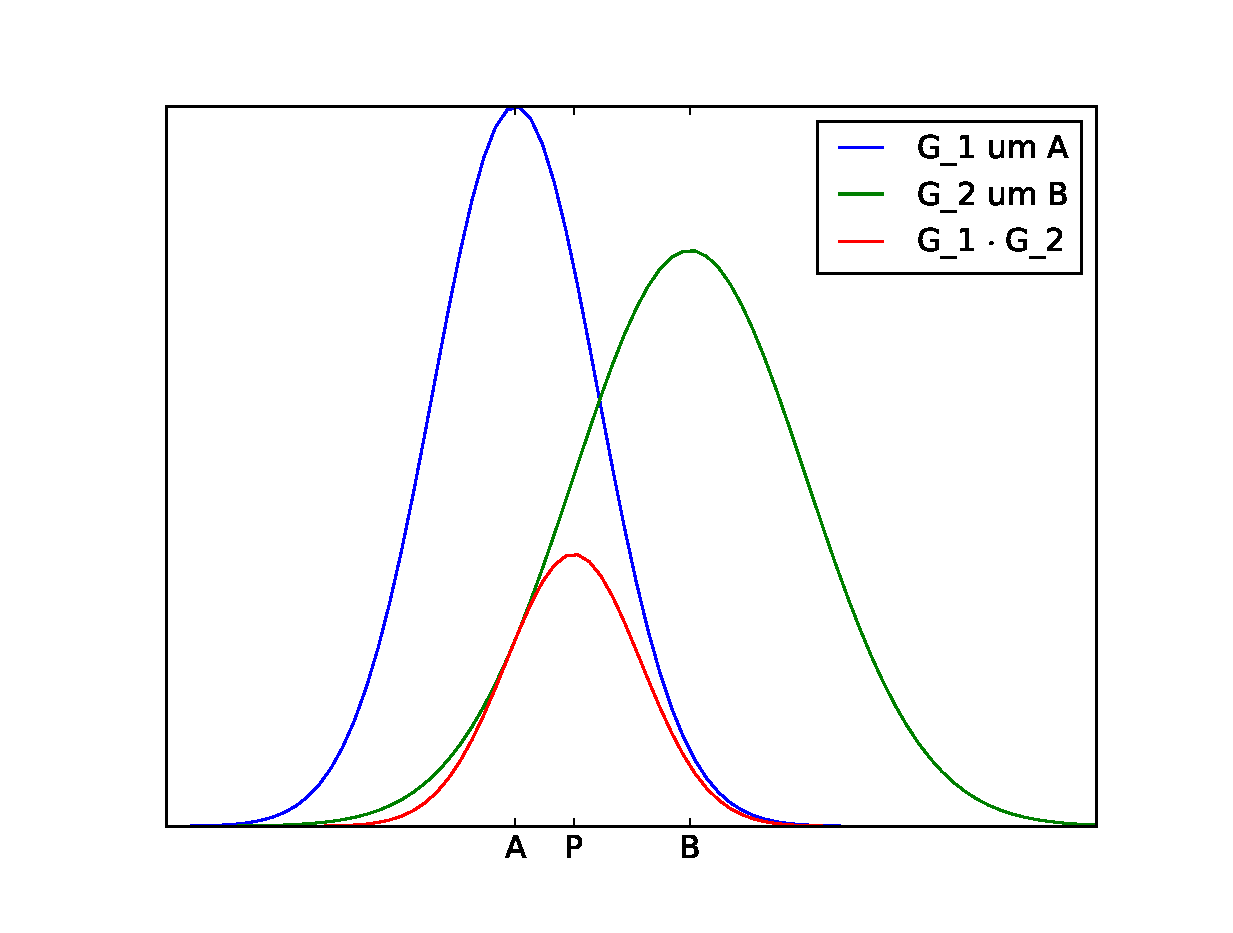
\includegraphics[scale=0.6]{GF.eps}
%	\vspace*{-7mm}
%	\caption{Eindimensionales Beispiel für das Produkt zweier beliebiger 
%	Gauß-Funktionen (vgl. \ref{eq:Produktansatz}). Die Lage des neuen Maximas 
%	ergibt sich durch 
%	\ref{eq:neuesZentrum_P}.}
%	\label{pic:1d_GTO} 
%\end{figure}
%
Dieses Vorgehen lässt sich beliebig oft wiederholen, was ein 
besonderer Vorteil für die oben erwähnten 4-Zentrenintegrale darstellt. Das 
Produkt von zwei nicht normierten GTOs lässt sich in eine 
Summe
%
\begin{align}
\psi_a(\textbf{r}_1)\cdot \psi_b(\textbf{r}_1) &=  x_A^i\,y_A^k\,z_A^m\cdot  
x_B^j\,y_B^l\,z_B^n\cdot e^{-b r_B^2-a 
		r_A^2}\\
%
&= \sum_{t=0}^{i+j}E^{i,j}_t\ 
\sum_{u=0}^{k+l}E^{k,l}_u\ \sum_{v=0}^{m+n}E^{m,n}_v\ 
\Lambda_{tuv}(\textbf{r}_1,p,\textbf{P})
\end{align}
%
über
%
\begin{align}
\Lambda_{tuv}(\textbf{r}_1,p,\textbf{P})&=\frac{\text{d}^t}{\text{d}P_x^t}\frac{\text{d}^u}{\text{d}P_y^u}\frac{\text{d}^v}{\text{d}P_z^v}\
 \exp(-p r_{1,P}^2)
\end{align}
%
schreiben.
Die nötigen Koeffizienten werden 
rekursiv mithilfe von
%
\begin{align}\label{eq:E:coef1}
E_0^{0,0}&=\exp(-\frac{ab}{p}(A_x-B_x)^2)\\\label{eq:E:coef2}
E_0^{i+1,j}&=-\frac{b}{p}(A_x-B_x)E^{i,j}_0 + E_1^{i,j}\\\label{eq:E:coef3}
E_0^{i,j+1}&=\frac{a}{p}(A_x-B_x)E^{i,j}_0 + E_1^{i,j}\\\label{eq:E:coef4}
E_t^{i,j} &= \frac{1}{2pt}\rl{iE^{i-1,j}_{t-1}+jE^{i,j-1}_{t-1} }
\end{align}
%
berechnet (siehe z.B. auch \cite{av:3a}), wobei das neue Zentrum durch
%
\begin{align}\label{eq:neuesZentrum_P}
p:=a+b \qquad, \qquad
\textbf{P}:=\frac{a\textbf{A}+b\textbf{B}}{p}
\end{align}
%
bestimmt ist. Eine analoge Umformung kann für das 
zweite Teilchen (\textbf{r}$_2$) mit
%
\begin{align}\label{eq:Q}
q:=c+d \qquad, \qquad
\textbf{Q}:=\frac{c\textbf{C}+d\textbf{D}}{q}
\end{align}
%
durchgeführt werden. Weiterhin zeigt Boys, dass alle Integrale dieses Typs eine 
%TODO ACHTUNG ZEILENTRENNUNG in finaler Version pruefen
|\textbf{P}-\textbf{Q}| Abhängigkeit haben, das heißt, dass sie nicht von den 
einzelnen Komponenten der Vektoren \textbf{P} und \textbf{Q} abhängen. Daher  
gilt 
%
$\rl{\frac{\DEL}{\DEL P_x}}^i = \rl{-\frac{\DEL}{\DEL 
Q_x}}^i=(-1)^i \rl{\frac{\DEL}{\DEL Q_x}}^i$
%
, was für das gesamt Integral bedeutet:
%
\begin{align}\label{eq:E:Koef}
I &= % N_{ikm}(a)N_{jln}(b)N_{i'k'm'}(c)N_{j'l'n'}(d) \cdot \\ 
%& \cdot 
\sum_{t=0}^{i+j}E^{i,j}_t\ \sum_{u=0}^{k+l}E^{k,l}_u\ 
\sum_{v=0}^{m+n}E^{m,n}_v\ (-1)^{t+u+v} \sum_{t'=0}^{i'+j'}E^{i',j'}_{t'}\ 
\sum_{u'=0}^{k'+l'}E^{k',l'}_{u'} \sum_{v'=0}^{m'+n'}E^{m',n'}_{v'}\ 
R^{t+t',u+u',v+v'}\ ,
\end{align}
%
wobei die gestrichenen Indizes für die Potenzen der GTO des 
zweiten Teilchens 
(\textbf{r}$_2$) stehen. Weiterhin wird die Schreibweise
% 
\begin{align}\label{eq:McM-D:kartesieAbleitungen}
R^{\tau,\rho,\sigma}&=\frac{d^\tau}{dQ^\tau_x}\ 
\frac{d^\rho}{dQ^\rho_y}\ \frac{d^\sigma}{dQ^\sigma_z}\ 
B\\\label{eq:basisint1}
B&= \int \int d\textbf{r}_1 d\textbf{r}_2 \ e^{-pr_{1,P}^2} \cdot 
f_{12}(r_{12}) \cdot e^{-qr_{2,Q}^2} \quad.
\end{align}
%
genutzt, wobei $B$ das sogenannte \textit{Basisintegral}  ist. Weiter wird dem 
McMurchie-Davidson Schema nicht gefolgt. 
%
%
%
\subsubsection{Analytische Modifikationen des Basisintegrals}\label{sec:modifik}
%
Als zweiten Schritt vereinfacht \cite{av:1a} das Basisintegral :
\begin{enumerate}
	\item[1.]  Es wird beobachtet, dass ,wie erwähnt, $B$ nur 
	von 
	|\textbf{P}-\textbf{Q}| abhängt. Daher kann nun eine 
	Koordinatenverschiebung 
	vorgenommen werden, sodass sich ein Punkt (z.B. \textbf{P}) im Ursprung 
	befindet\footnote{Im folgenden wird \textbf{Q}$_\text{neu}$ weiterhin mit 
	\textbf{Q} bezeichnet.}.\\
	$\Rightarrow \ \textbf{P}_\text{neu2}=0\ , \qquad 
	\textbf{Q}_{\text{neu}}=\textbf{Q}-\textbf{P}$
	%
	%
	\item[2.] Anschließend wird die noch verschobene Gauß-Funktion in 
	Kugelflächenfunktionen und modifizierte sphärische Besselfunktionen der 
	ersten Art entwickelt. Es gilt:
	\begin{align}
	e^{-qr_{2,Q}^2}=4\pi 
	e^{-qQ^2}\sum_{l=0}^{\infty}i_l(2qQr_2)\sum_{m=-l}^{+l} 
	Y_{lm}^*(\hat{Q})Y_{lm}(\hat{r}_2) \quad,
	\end{align}
	wobei $Q=|\textbf{Q}|$ ist. Diese Gleichung kann durch 
	die Verwendung von zum Beispiel \cite{b:5a} gezeigt 
	werden.
	Da über den gesamten Raum integriert wird, entfallen aus  
	Symmetriegründen 
	alle Terme außer l=0 ($\rightarrow$ m=0). Daher verbleibt B bei
	\begin{align}\label{eq:Basisintegral:zwerg}
	B=e^{-qQ^2} \int \int d\textbf{r}_1 d\textbf{r}_2\ e^{-pr_1^2-qr_2^2} 
	\frac{\sinh(2qQr_2)}{2qQr_2}\cdot f_{12}(r_{12}) \quad .
	\end{align}
	%
	%
	\item[3.] Als letzte Umformung wird eine Koordinatentransformation 
	durchgeführt. Hierbei geht man in ein System, indem ein Teilchen  im 
	Ursprung und das zweite auf der z-Achse liegt. Anschließend geht man in 
	Kugelkoordinaten. Die daraus resultierende Integralbildung wird z.B. in 
	\cite{av:6a} beschrieben. 
	%
	\begin{align*}
	\{x_1,y_1,z_1,x_2,y_2,z_2\}\rightarrow\{r_1,r_2,r_{12},\alpha,\beta,\gamma\}
	\end{align*}
	%
	
	$\alpha,\beta$ und $\gamma$ sind resultierende Eulerwinkel, die entstehen, 
	wenn das Koordinatensystem 1 (\textbf{r}$_1$) derart 
	gedreht wird, dass 
	der Vektor \textbf{r}$_2$ auf der z-Achse liegt. 
	Weiterhin muss erwähnt werden, dass offensichtlich d\textbf{r}$_1$ = 
	d\textbf{r}$_{12}$ gilt, wodurch sich im Gegensatz zu \cite{av:6a} die 
	Bedeutung von $r_1$ und	$r_{12}$ vertauscht. 
	Da außerdem $r_1=|\textbf{r}_{12}+\textbf{r}_2|$ gilt, 
	folgt nach elementarer Winkelintegration für allgemeine Funktionen f,g und 
	h:
	\footnote{$\textbf{r}_1=\textbf{r}_{12}+\textbf{r}_{2},\ 
		r_1=\sqrt{r_{12}^2+r_2^2-2r_{12}r_2\cos(\beta)},\ 
		d\textbf{r}_{12}= r^2_{12} \sin(\beta) \ dr_{12}\ d\alpha\ d\beta$} 
%
	\begin{align}\nonumber
		\int \int & f(r_{1}) g(r_2)h(r_{12}) d\textbf{r}_1d\textbf{r}_2 =\\
		% 
		& 8\pi^2\int_{0}^{\infty}h(r_{12})\ r_{12}\ dr_{12}\int_{0}^{\infty} 
		g(r_2)\ r_2\ dr_2 \int_{|r_{12}-r_2|}^{r_{12}+r_2}f(r_{1})\ r_{1}\ 
		dr_{1}\quad.
	\end{align}
	Nach Integration (vergleiche \ref{eq:Basisintegral:zwerg} ) über $r_1$ und 
	$r_2$ verbleibt
	\begin{align}\label{eq:B:zwischenErg}
		B= \sqrt{\frac{\pi^5}{p+q}}\frac{1}{pq}\cdot \int_{0}^{\infty}dr_{12}\ 
		f_{12}(r_{12})\cdot r_{12}\cdot \rl{\frac{e^{-  
		\frac{pq}{p+q}(r_{12}-Q)^2}-e^{-\frac{pq}{p+q}(r_{12}+Q)^2}}{Q}}\quad .
	\end{align}
\end{enumerate} 
%
Im Folgenden wird die zusammenfassende Größe
%
\begin{align}
\xi := \frac{p\cdot q}{p+q}
\end{align}
%
verwendet, um \ref{eq:B:zwischenErg} zu vereinfachen.
%
%
%
\subsubsection{Hobson Theorem und 
Schlegel-Koeffizienten}\label{sec:Hobson_schlegel}
%
Wie in \ref{eq:McM-D:kartesieAbleitungen} zu erkennen ist, müssen  
Ableitungen des Basisintegrals berechnet werden\footnote{In der Arbeit 
\cite{av:9a} ist eine genauere und z.T. berichtigte Version dieses Teils des 
Algorithmus aus \cite{av:1a} beschrieben.}. Da B nur von $Q=|Q|$ abhängt, 
ist es sinnvoll, die kartesischen Ableitungen in sphärische Ableitungen nach 
$Q$ umzuformen.\\
Dazu wird als Erstes auf die Arbeit \cite{av:4a} verwiesen, in der ein 
vollständiger, analytischer Ausdruck für die Umformung von sphärische in  
kartesische GTOs (Koordinatenwechsel des polynomartigen Anteils) präsentiert 
wird. Die Rückumformung, das heißt die Umformung von kartesischen in 
sphärische Koordinaten, kann nach Absprache mit den Autoren von \cite{av:1a} 
wie folgt dargestellt werden. Sind $c_{l_xl_yl_z}^{l,m}$ die reellen 
Schlegel-Koeffizienten aus \cite{av:4a}, so können die Koeffizienten der 
Rückumformung mit
%
\begin{align}\nonumber
c^{-1}(l,m,l_x,l_y,l_z)&=\frac{2}{\Gamma\rl{\frac{l_x+l_y+l_z+l+3}{2}}} 
 \ \cdot \\ \label{eq:def:c_koef}
 &\cdot  \sum_{a+b+c\leq l} c_{l_xl_yl_z}^{lm}\cdot 
\Gamma\rl{\frac{1+l_x+a}{2}}\cdot 
\Gamma\rl{\frac{1+l_y+b}{2}}\cdot \Gamma\rl{\frac{1+l_z+c}{2}}
\end{align}
%
berechnet werden. Damit ist also die Umformung
%
\begin{align}\label{eq:trafo_c-1}
x^{l_x}y^{l_y}z^{l_z} = \sum_{l=0}^{l_{max}}\sum_{m=0}^l 
c^{-1}(l,m,l_x,l_y,l_z)\cdot r^{l_{max}-l} Z_{lm}(\textbf{r})
\end{align}
%
möglich. $Z_{lm}(\textbf{r})=r^l\cdot Y_{lm}(\hat{\textbf{r}})$ sind die 
reellen, soliden 
Kugelflächenfunktionen ohne Racah's Normalisierung und 
$l_{max}=l_x+l_y+l_z$. Eine detailliertere Beschreibung inkl. aller 
Definitionen bzgl. dieser Transformation ist im Anhang 
\ref{sec:AnhangA:Schlegel} zu finden. Weiterhin sei erwähnt, 
dass auch 
\cite{av:4a} einige kleinere Tippfehler hat, welche in Anhang berichtigt sind.\\

Analog dazu können mithilfe der selben Koeffizienten auch die 
Differenzialoperatoren \ref{eq:McM-D:kartesieAbleitungen} umgeformt werden. 
Mit der Verwendung des Hobson Theorems in der Form
%
\begin{align}\label{eq:Hobson}
\Op{Z}_{lm}(\nabla_Q)g(Q)=\left[\mathcal{D}^l_Qg(Q)\right]Z_{lm}(\textbf{Q}) 
\end{align}
%
können die kartesischen Ableitungen durch 
%
\begin{align}
R^{\tau,\rho,\sigma}=\frac{d^\tau}{dQ^\tau_x}\ 
\frac{d^\rho}{dQ^\rho_y}\ \frac{d^\sigma}{dQ^\sigma_z}\ 
B=\sum_{l=0}^{l_{max}}\sum_{m=-l}^{l}c^{-1}(l,m,\tau,\rho,\sigma)\cdot
 \nabla_Q^{l_{max}-l}\left[(\mathcal{D}_Q^lB)Z_{lm}(\textbf{Q})\right]
\end{align}
%
ausgedrückt werden, wobei $\mathcal{D}^l_Q=Q^{-1}\DEL_Q$ darstellt. Ist  
$l_{max}-l$ 
ungerade, so ist $c^{-1}=0$. Mithilfe der Relation 
$\nabla_Q^2=Q^2\mathcal{D}^l_Q+3\mathcal{D}_Q$ 
kann nun \ref{eq:McM-D:kartesieAbleitungen} in die finale Form
%
\begin{align}\label{eq:final:Hobson}
R^{\tau,\rho,\sigma}=\sum_{l=0}^{l_{max}}\sum_{m=-l}^{l}c^{-1}(l,m,\tau,\rho,\sigma)Z_{lm}(\textbf{Q})
 \sum_{k=0}^{k_{max}}d_k^{l,k_{max}} \cdot 
\left[(\mathcal{D}_Q^{l_{max}-k}B)\right]Q^{l_{max}-l-2k}
\end{align}
%
geschrieben werden. Hierbei ist $k_{max}=\frac{1}{2}(l_{max}-l)$ und die 
Koeffizienten $d_k^{l,k_{max}}$ können rekursiv berechnet werden:
%
\begin{align}\nonumber
d_n^{l,m}=d_n^{l,m-1} &+\left[2l+3+4(m-n)\right]d_{n-1}^{l,m-1}+\\ 
\label{eq:rek_d}
&2(m-n+1)(2l+3+2(m-n))d_{n-2}^{l,m-1} \qquad.
\end{align} 
%
Die Rekursion startet bei $d_{-1}^{l,m}=0$ und $d_0^{l,m}=1$.
%
%
%
\subsubsection{Radiale Ableitungen der Basisintegrale}
%
Der letzte in der Arbeit \cite{av:1a} präsentierte Schritt 
sieht die 
Evaluation der radialen Ableitungen des Basisintegrals vor. Dazu werden zwei 
Vorgehensweisen dargestellt. Die erste in der vorliegenden 
Arbeit nicht 
behandelte Vorgehensweise nutzt eine Taylorentwicklung\footnote{In den Formeln 
(44)-(46) von \cite{av:1a} ist bei der Umformung der Exponentialfunktionen in 
den sinh ein Faktor 2 verlorengegangen. Weiterhin fehlt im 
ersten Term von 
(47) ein weiterer Faktor 2.} von $Q$ um 0 aus. Da im Regime der ultrakalten 
Gase der Bereich von sehr kleinen Teilchenabständen ($Q$) eher uninteressant 
ist\footnote{Da in diesem Bereich die harmonische Falle vernachlässigt werden 
kann und die Schrödingergleichung in Relativ- und Schwerpunktkoordinaten 
separiert und somit in 1D lösbar ist.}, wird nun das zweite Vorgehen für 
mittlere und große $Q$ erläutert.\\

Das Basisintegral \ref{eq:Basisintegral:zwerg} kann in zwei Terme 
geschrieben werden. Mithilfe der Definition 
%
\begin{align}
\mathcal{H}^\pm_{jkl}&:=\sqrt{\frac{\pi^5}{p+q}}\frac{1}{pq} \int_{0}^{\infty} 
dr_{12}\ r_{12}^j\ \cdot 
\rl{\frac{1}{Q}\frac{\text{d}}{\text{d}Q}}^l\rl{\frac{e^{-\xi(r_{12}\pm 
			Q)^2}}{Q^k}}
\end{align}
%
gilt
%
\begin{align}\label{eq:diff_op}
\mathcal{D}_Q^lB=\left[\rl{\frac{1}{Q}\frac{d}{dQ}}^lB\right] 
=\rl{\mathcal{H}^-_{11l}-\mathcal{H}^+_{11l}} \quad .
\end{align}
%
Durch abermalige Anwendung des Differentialoperators $\mathcal{D}_Q$ kann die 
Rekursion
%
\begin{align}\label{eq:rek:H}
\mathcal{H}_{jkl}^{\pm} = \mp 2\xi\cdot \mathcal{H}_{j+1,k+1,l-1}^\pm-2\xi\cdot 
\mathcal{H}_{j,k,l-1}^\pm-k\cdot\mathcal{H}_{j,k+2,l-1}^\pm
\end{align}
%
gefunden werden. Man beobachtet, dass auf Kosten von j und k der Index l für 
die Ableitungen reduziert werden kann. Durch die trivialen Relationen
\begin{align} \label{eq:prop:H}
\mathcal{H}_{jk0}^{\pm} &= \frac{1}{Q^k} \cdot \mathcal{H}_{j00}^\pm\\ 
\mathcal{H}_{j00}^{\pm} &=\sqrt{\frac{\pi^5}{p+q}}\frac{1}{pq} \cdot \Pi_j^\pm
\end{align}
vereinfacht sich das nun noch zu berechnende Integral auf
\begin{align}\label{eq:PI-Integrale}
\Pi_j^\pm= \int_{0}^{\infty}dr_{12}\ r_{12}^j \cdot f_{12}(r_{12}) \cdot 
e^{-\xi (r_{12} \pm Q)^2}\quad .
\end{align}
%
%
%
\subsubsection{Zusammenfassung}\label{sec:Zusammenfassung:Algorithmus}
%
Ziel des Algorithmus ist es gewesen, 
%
\begin{align}\nonumber
I= \int \int\ 
d\textbf{r}_1\ d\textbf{r}_1 
(\psi_i^a(\textbf{r}_1)\psi_i^c(\textbf{r}_2))^* f_{12}(r_{12}) 
\psi_j^b(\textbf{r}_1)\psi_j^d(\textbf{r}_2)
\end{align}
%
zu berechnen. Mithilfe des Ansatzes der GTOs kann die Integralberechnung   
auf die Schar der $\Pi_j^\pm$ Integrale \ref{eq:PI-Integrale}
%
\begin{align}\nonumber
\Pi_j^\pm= \int_{0}^{\infty}dr_{12}\ r_{12}^j \cdot f_{12}(r_{12}) \cdot 
e^{-\xi (r_{12} \pm Q)^2}
\end{align}
% 
zurückgeführt werden. Wichtig hierbei ist die korrekte Definition von $Q$ 
(\ref{eq:Q}) mit Berücksichtigung der Koordinatenverschiebung in 
\ref{sec:modifik}, bei der P auf den Ursprung verschoben 
wird. Anschließend 
ermittelt man mithilfe der Rekursion \ref{eq:rek:H}
%
\begin{align}\nonumber
\mathcal{H}_{jkl}^{\pm} = \mp 2\xi\cdot \mathcal{H}_{j+1,k+1,l-1}^\pm-2\xi\cdot 
\mathcal{H}_{j,k,l-1}^\pm-k\cdot\mathcal{H}_{j,k+2,l-1}^\pm
\end{align}
%
und den benötigten Proportionalitäten \ref{eq:prop:H} die Integrale 
$\mathcal{H}_{11l}^\pm$. \\
Via \ref{eq:final:Hobson} mit \ref{eq:diff_op}
%
\begin{align}\label{R_sum}
R^{\tau,\rho,\sigma}=\sum_{l=0}^{l_{max}}\sum_{m=-l}^{l}c^{-1}(l,m,\tau,\rho,\sigma)Z_{lm}(\textbf{Q})
\sum_{k=0}^{k_{max}}d_k^{l,k_{max}} \cdot 
\left[(\mathcal{H}^-_{11l}-\mathcal{H}^+_{11l})\right]Q^{l_{max}-l-2k}
\end{align}
%
und \ref{eq:E:Koef} 
%
\begin{align}\nonumber 
I &= %N_{ikm}(a)N_{jln}(b)N_{i'k'm'}(c)N_{j'l'n'}(d) \cdot \\ \nonumber
%& \cdot 
\sum_{t=0}^{i+j}E^{i,j}_t\ \sum_{u=0}^{k+l}E^{k,l}_u\ 
\sum_{v=0}^{m+n}E^{m,n}_v\ (-1)^{t+u+v} \sum_{t'=0}^{i'+j'}E^{i',j'}_{t'}\ 
\sum_{u'=0}^{k'+l'}E^{k',l'}_{u'} \sum_{v'=0}^{m'+n'}E^{m',n'}_{v'}\ 
R^{t+t',u+u',v+v'}
\end{align}
%
ist das Integral berechnet. \\

Dieses Vorgehen ist unabhängig von der Form der eingesetzten Funktion 
$f_{12}(r_{12})$, solange die Abhängigkeit $r_{12}=|\textbf{r}_1-\textbf{r}_2|$ 
stimmt. $\Pi^\pm_j$ kann sowohl analytisch als auch im Allgemeinen numerisch 
gelöst werden. Auf mögliche Probleme dabei wird im folgenden Abschnitt 
eingegangen. Die Normierungskonstanten $N$ können ohne Beschränkung der 
Allgemeinheit auch weggelassen werden. Dies entspricht der Verwendung von 
nicht normierten GTOs als Basisfunktionen.
%
%
%
\subsection{Berechnung der Basisintegrale}
%
Dieser Abschnitt widmet sich der Betrachtung der $\Pi_j^\pm$-Integrale. Im 
Regime der ultrakalten Gase und unter der Verwendung des Hamiltonoperators 
\ref{eq:kernHam1} ist leicht zu sehen, dass die Funktion $f_{12}$ die 
Ortsdarstellung des Wechselwirkungsoperators 
($\hat{=}$Wechselwirkungspotential) 
$\Op{U}(r_{12})$ darstellt. Alle restlichen Operatoren 
bedürfen keiner 
Zweiteilchenintegralen. Prinzipiell ist der Algorithmus auch für 
Einteilchenintegrale benutzbar, jedoch soll vorher geprüft 
werden, ob andere 
existierende Einteilchenintegral-Algorithmen nicht effektiver 
sind\footnote{Außerdem muss die Implementierung im Kapitel 
\ref{sec:Implementierung} entsprechend angepasst werden.}.\\
Für das oben beschriebene System ist kein analytisches 
Wechselwirkungspotential bekannt. Aus numerischen Elektronenstrukturrechnungen 
und Experimenten kann jedoch ein numerisches Potential angegeben werden 
\cite{phdthesis:sergey}. Ein Problem im Regime der 
ultrakalten Gase ist,  dass Wechselwirkungspotentiale eine 
Divergenz im Ursprung haben. Diese entstehen aus dem Fakt, dass zwei Atome 
nicht am exakt selben Ort sein können. Die Wellenfunktion muss aus 
physikalischer Sicht dort exakt Null sein und im Bereich des starken Anstiegs 
des Potentials exponentiell abfallen. Die GTOs erfüllen diese Randbedingungen 
im Allgemeinen nicht. Daher ist die prinzipielle Divergenz in $\Pi^\pm_j$ nicht 
überraschend. Eine rein numerische Funktion $f_{12}$ mit Divergenz in 0 ist 
damit für das Integral nur schwer anwendbar. Die 
Basisfunktionen müssen so 
gewählt werden, dass die Divergenz nicht zum Tragen kommt, 
das heißt, dass der 
"Flächeninhalt"\ direkt um 0 zu vernachlässigen ist. Die 
Basisfunktionen müssen 
dort also im Rahmen der Numerik verschwinden.\\%TODO vlt ein Bild zeigen 
%beidem ein   %solcher Fall gezeigt ist.
Weiterhin kann versucht werden, die numerische Integration zu 
renormieren, indem 
zum Beispiel nicht bis exakt 0, sondern zu einem speziellen Wert $\epsilon>0$  
integriert wird. Das Problem hierbei ist, $\epsilon$ so zu bestimmen, dass das 
Integral noch alle benötigten Informationen enthält und so ein physikalisch 
sinnvolles Ergebnis entsteht. Da dieses Vorgehen eher ungenau und $\epsilon$ 
numerisch noch nicht motiviert ist, wird dieses Vorgehen hier nicht weiter 
verfolgt.\\
Ein dritter Weg stellt eine analytische Funktion für $f_{12}$ dar, das heißt 
eine durch Parameter optimierte Näherungsfunktion für das numerische Potential 
(ein Fit ). Zwei bekannte Näherungsfunktionen für ein numerisches 
Wechselwirkungspotential zwischen Atomen stellen das 
Lennard-Jones- (kurz LJP) 
und das Morse-Potential (kurz MRP) dar. Beide haben qualitativ
einen ähnlichen Verlauf und sind in der Quantenchemie gebräuchlich.\\
Vorteil des Lennard-Jones-Potentials ist das korrekte asymptotische Verhalten 
für große Abstände mit $\sim -\frac{C}{r^6}$, wobei C ein 
Van-der-Waals-Koeffizient darstellt. Dagegen hat das Morse-Potential eine etwas 
einfachere mathematische Form. Beide können durch Angabe der erwarteten 
(gemessenen) Dissoziationsenergie und der Lage des Minimums 
bestimmt 
werden. Das Morse-Potential hat außerdem einen weiteren 
Parameter, den 
Exponenten, der die Steilheit bzw. auch Steifheit genannt, 
der Kurve 
manipuliert.\\

Im Folgenden werden beide hier erwähnten Potentiale erklärt und im Rahmen des 
$\Pi^\pm_j$ Integrals diskutiert und berechnet.
%
%
%
\subsubsection{Wechselwirkungspotentiale:}
\subparagraph{Das Morse-Potential} hat die drei Schreibweisen  
%
\begin{align}\label{eq:MRP}
V_{\text{MRP}}(r_{12}) &= D_e\cdot \rl{1-e^{-a_\text{st}\cdot(r_{12}-R_m)}}^2 
-D_e\\
                       &= D_e\cdot 
                       \rl{e^{-2a_\text{st}(r_{12}-R_m)}-2e^{-a_\text{st}(r_{12}-R_m)}}\\
                       &=A_{\text{MRP}}\cdot e^{-2a_\text{st} r_{12}} + 
                       B_{\text{MRP}}\cdot e^{-a_\text{st} r_{12}} \quad,
\end{align}
%
wobei $D_e$ die Dissoziationsenergie , $R_m$ die Lage des Minimums und $a$ ein 
an sich beliebiger positiver reeller Parameter ist.  Die Koeffizienten 
$A_\text{MRP} \text{ und  }B_\text{MRP}$ können als Zusammenfassung vieler 
Parameter 
aufgefasst werden, um die numerische Behandlung zu vereinfachen. \\
Das folgende Bild (\ref{pic:MRP_1}) veranschaulicht das Morse-Potential und die 
Abhängigkeit 
bzgl. des Exponenten.
%
%\begin{figure}[H] \centering
%	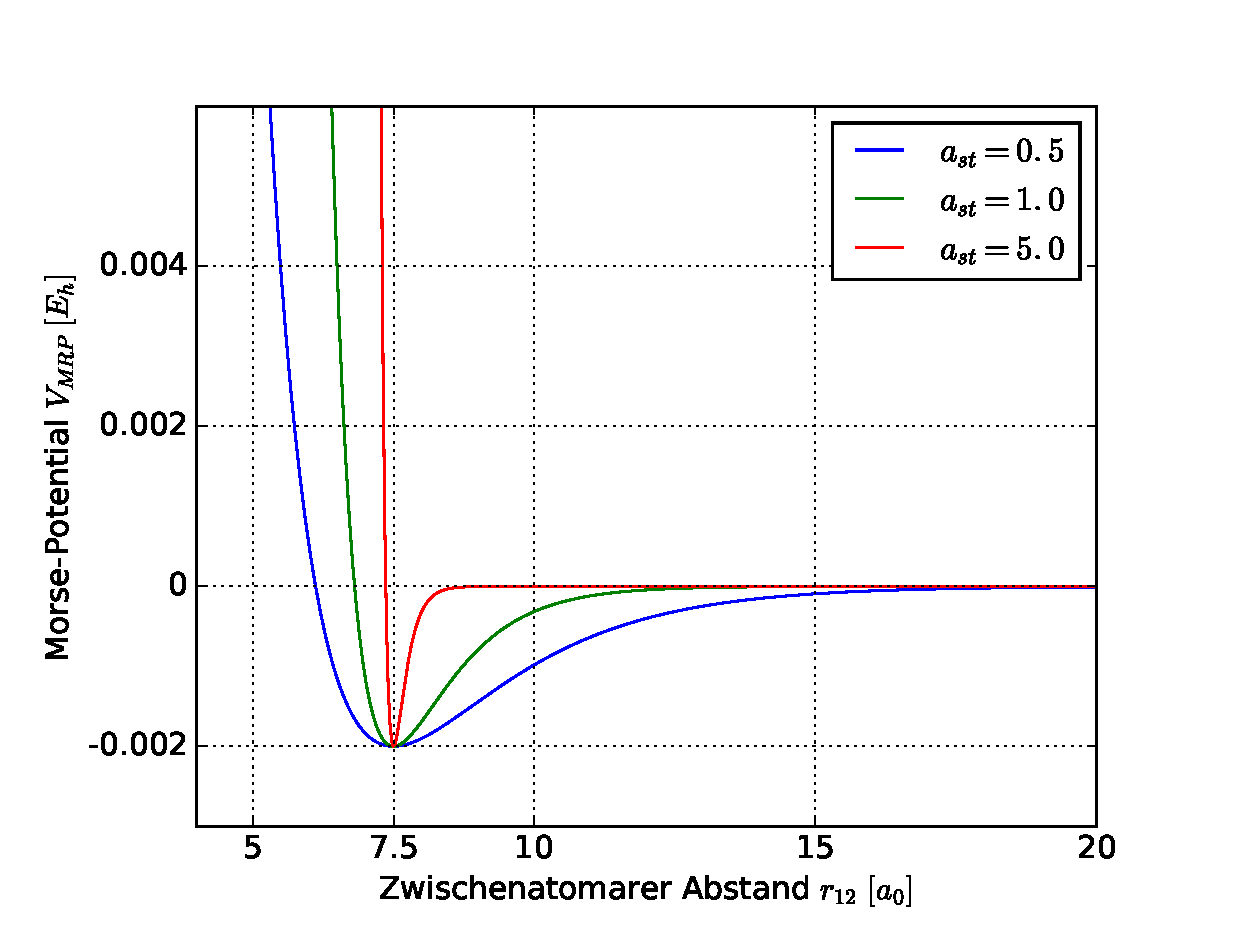
\includegraphics[scale=0.65]{MRP.eps}
%%	\vspace*{-10mm}
%	\caption{Es ist das Morse-Potential \ref{eq:MRP} mit fixierten Parametern 
%	$D_e = 0.002\ E_h$ und $R_m = 7.5\ a_0$ zu verschiedenen Exponenten 
%	$a_\text{st}$ im 
%	Bereich von 0.5 bis 5.0 dargestellt.}%TODO anderes Bild / vorallem andere 
%	%achsenbeschreiftungen !!!
%	\vspace{2mm} %\hrule 
%	\label{pic:MRP_1} 
%\end{figure}
%
Nun soll das Morsepotential als Funktion $f_{12}$ in das $\Pi^\pm_j$ - 
Integral  \ref{eq:PI-Integrale} eingesetzt werden:
%
\begin{align}
\Pi_j^\pm & =\int_{0}^{\infty}dr_{12}\ r_{12}^j \cdot V_\text{MRP}(r_{12}) \cdot
           e^{-\xi (r_{12} \pm Q)^2}\\
          & = \int_{0}^{\infty}dr_{12}\ r_{12}^j \cdot \rl{A_{\text{MRP}}\cdot 
          e^{-a_\text{st} r_{12}} + B_{\text{MRP}}\cdot e^{-2a_\text{st} 
          r_{12}}} \cdot e^{-\xi 
          (r_{12} \pm Q)^2} \\ \label{eq:PI_MRP}
          & = A^\prime_{\text{MRP}}\cdot \int_{0}^{\infty}dr_{12}\ r_{12}^j 
          \cdot e^{b_1\cdot r_{12} - \xi r_{12}^2} + B^\prime_\text{MRP}\cdot 
          \int_{0}^{\infty}dr_{12}\ r_{12}^j \cdot e^{b_2\cdot r_{12} - \xi 
          r_{12}^2}
\end{align}
%
Hierbei sind die Parameter $A^\prime_\text{MRP},\ B^\prime_\text{MRP},\ b_1$ 
und $b_2$ Zusammenfassungen von Konstanten. Diese sind durch
%
\begin{align}
A^\prime_\text{MRP}&:=A_\text{MRP}\cdot e^{-\xi Q^2}= D_e\cdot 
e^{2a_\text{st}R_m} \cdot 
e^{-\xi Q^2}\\
B^\prime_\text{MRP}&:=B_\text{MRP}\cdot e^{-\xi Q^2}= -2\cdot D_e\cdot 
e^{a_\text{st}R_m} 
\cdot e^{-\xi Q^2}\\
b_1 &:=-(a_\text{st}\pm 2\xi Q)\\
b_2 &:=-2(a_\text{st} \pm \xi Q )
\end{align}
%
definiert. Wie man an \ref{eq:PI_MRP} erkennt, kann das $\Pi^\pm_j$-Integral 
durch ein verallgemeinertes Integral über ein Monom des Grades j und einer 
Exponentialfunktion berechnet werden. Die Evaluation des Integraltyps
%
\begin{align}\label{eq:def:S}
S(\alpha,\beta,\gamma):=\int_{0}^{\infty}\ dx\ x^\alpha\cdot e^{\beta x - 
\gamma 
x^2}
\end{align}
%
wird im Abschnitt III.B-C der Arbeit \cite{av:1a} diskutiert. Für 
$\alpha\geq-1$, $\alpha\in \mathbb{N}, (\beta,\gamma)\in\mathbb{R}$ und $\gamma 
>0$  kann das Integral 
regulär berechnet werden. Für das MRP sind diese Forderungen immer 
erfüllt\footnote{da $\alpha=j$ wobei $j\in \mathbb{N}$ und $j\geq1$ mit 
$\beta=\{b_1,b_2\}$ und $\gamma=\xi$}, sodass das Integral ohne 
weitere Näherungen berechnet werden kann. $\Pi_j^\pm$ lässt sich damit 
also 
durch
%
\begin{align}\label{eq:PIinS_MRP}
\Pi^\pm_j=A^\prime_\text{MRP}\cdot 
S(j,b_1,\xi)+B^\prime_\text{MRP}\cdot 
S(j,b_2,\xi)
\end{align}
%
ausdrücken. In dieser Arbeit wird S mithilfe von 
%
\begin{align}\nonumber
S(\alpha,\beta,\gamma)  
&=(2\sqrt{\gamma})^{-\alpha-1}\Gamma(\alpha+1)\sqrt{\pi}\cdot
\left[\frac{M\rl{\frac{\alpha+1}{2},\frac{1}{2},\frac{\beta^2}{4\gamma}}}{\Gamma(\alpha/2+1)}
+\frac{\beta}{\sqrt{\gamma}} 
\frac{M\rl{\frac{\alpha}{2}+1,\frac{3}{2},\frac{\beta^2}{4\gamma}}}{\Gamma((\alpha+1)/2)}\right]\\\nonumber
%
&=\frac{1}{2}\, \gamma^{-1 - \frac{\alpha}{2}}\cdot \bigg[\beta\cdot 
\Gamma\rl{1 + \frac{\alpha}{2}}M\rl{1 + \frac{\alpha}{2}, \frac{3}{2}, 
\frac{\beta^2}{4\gamma}} \\ \label{eq:S,alpha>0}
&\qquad \qquad \qquad +\sqrt{\gamma}\cdot \Gamma\rl{\frac{1+\alpha}{2}}\cdot 
M\rl{\frac{1 + 
\alpha}{2}, 
\frac{1}{2},\frac{\beta^2}{4\gamma}} \bigg]
\end{align}
%
berechnet, wobei M Krummers konfluierte hypergeometrische Funktion ( auch mit 
$_1F_1$ bezeichnet) darstellt. Diese wird wiederum durch die 
Reihendarstellung 
%
\begin{align}\label{eq:reihe_M_kon.hyp.geo}
M(a,b,z)=1+\frac{az}{b}+\frac{(a)_2z^2}{(b)_2 
2!}+\dots +\frac{(a)_nz^n}{(b)_nn!}+\dots
\end{align}
mit den Pochhammer-Symbol
\begin{align}
(a)_n=a(a+1)(a+2)\dots(a+n-1), \ (a)_0=1
\end{align}
% 
berechnet (vergleiche mit \cite{b:1a} und \cite{b:6a}).\\
Erwähnt werden muss an dieser Stelle, dass \cite{av:1a} eine leicht andere 
Formel verwendet wird. In dieser Stelle findet Tricomis 
konfluierte 
hypergeometische Funktion 
($\mathcal{U}$) ihre Anwendung. Jedoch kann mit den im 
Vorfeld benutzten 
Konversionen  ( Definition (57) = Formel \ref{eq:def:S} ) die entsprechende 
Gleichung (60) aus \cite{av:1a} nicht abgeleitet werden\footnote{Es 
konnte 
sogar mithilfe eines kleinen MATHEMATICA-Skrips gezeigt werden, dass 
die linke 
Seite nicht der rechten entspricht. Durch Änderung der Definition 
\ref{eq:def:S} ($\beta\rightarrow-\beta$) und Vergleich mit 
\cite{b:6a} kann 
eine beinahe Übereinstimmung gefunden werden, jedoch müsste 
diese noch 
genauer 
geprüft und alle darauf folgenden Gleichungen in \cite{av:1a} 
angepasst werden. 
In dieser Arbeit wird diese Korrektur nicht weiter 
verfolgt.}. 
Dementsprechend wird 
auch nicht, der im unterstützenden Material \cite{av:1a2} 
dargestellte 
Weg zur Berechnung von $\mathcal{U}$ verwendet. Dieser berechnet $\mathcal{U}$ 
in verschiedenen Intervallen mit jeweils anderen Formeln, um die Konvergenz und 
Genauigkeit zu verbessern. Daher ist zu erwarten, dass auch 
\ref{eq:S,alpha>0} nicht für alle Bereiche der Parameter numerisch stabile 
Ergebnisse liefert\footnote{Es wird auch eine Integration 
durch quadratische 
Ergänzung des Exponenten und anschließender Umformung auf eine Erf-Funktion 
bzw. unvollständige $\Gamma$-Funktion 
versucht. Jedoch liefert dieses Vorgehen eine zu ungenaue 
Berechnung, da bei 
der auftretenden Subtraktion $1-\text{Erf}(x)$ schnell 
signifikante Stellen verloren gehen.}. Getestet wird diese Erwartung in Kapitel 
\ref{sec:Implementierung}. % (??) 
%
%
%
\subparagraph{Das Lennard-Jones-Potential} hat vor allem zwei gängige 
Darstellungen. Es muss erwähnt werden, dass in dieser Arbeit das sogenannte 
(12,6)-LJP benutzt wird:
%
\begin{align}\label{eq:def:LJP}
V_{\text{LJP}}(r_{12})&=D_e\cdot\left[ \rl{\frac{R_m}{r_{12}}}^{12} - 
2\rl{\frac{R_m}{r_{12}}}^6 \right]\\
                      &= 
                      \frac{A_\text{LJP}}{r_{12}^{12}}+\frac{B_\text{LJP}}{r^6_{12}}
                       \quad.
\end{align}
$D_e$ und $R_m$ sind analog zum MRP definiert. Auch $A_\text{LJP}$ und 
$B_\text{LJP}$ sind Zusammenfassungen von Konstanten:
%
\begin{align}
A_\text{LJP} &= D_e\cdot R_m^{12} \\
B_\text{LJP} &= -2\cdot D_e \cdot R_m^6 
\end{align}
%
Die Potenzen 12 bzw. 6 entstehen durch die betrachtete Wechselwirkung und 
Eigenschaften der Teilchen. Für neutrale, homonukleare Atome entsteht die 
Van-der-Waals Anziehung, die gut durch eine inverse sechste 
Potenz beschrieben 
werden kann. Der hier verwendete abstoßende Term mit der 
zwölften Potenz ist die
Konversion und kann im Zweifelsfall noch variiert werden. Im Gegensatz zum MRP 
hat das LJP in dieser Form keinen weiteren freien Parameter.\\
Für das $\Pi^\pm_j$-Integral ergibt sich:
%
\begin{align}
\Pi_j^\pm & =\int_{0}^{\infty}dr_{12}\ r_{12}^j \cdot V_\text{LJP}(r_{12}) \cdot
             e^{-\xi (r_{12} \pm Q)^2}\\\nonumber
          & = \int_{0}^{\infty}dr_{12}\ r_{12}^j \cdot 
          \rl{\frac{A_\text{LJP}}{r_{12}^{12}}+\frac{B_\text{LJP}}{r^6}}\cdot
          e^{-\xi (r_{12} \pm Q)^2}\\\nonumber
%\end{align}
%\begin{align}
%\Pi_j^\pm 
& = A^\prime_\text{LJP}\int_{0}^{\infty}dr_{12}\ r_{12}^j \cdot 
\frac{1}{r_{12}^{12}}\cdot e^{\mp 2\xi Q r_{12} -\xi r_{12}^2}+ 
B^\prime_\text{LJP}\int_{0}^{\infty}dr_{12}\ r_{12}^j 
\cdot\frac{1}{r_{12}^6}\cdot e^{\mp 2\xi Q r_{12} -\xi 
r_{12}^2}\\\nonumber
&=A^\prime_\text{LJP}\int_{0}^{\infty}dr_{12}\ r_{12}^{j-12}\cdot e^{\mp 2\xi Q 
r_{12} -\xi r_{12}^2}+ 
B^\prime_\text{LJP}\int_{0}^{\infty}dr_{12}\ r_{12}^{j-6}\cdot e^{\mp 2\xi Q 
r_{12} -\xi r_{12}^2}\\\label{eq:PI_LJP}
&=A^\prime_\text{LJP}\cdot 
S(\alpha_1,\beta,\gamma)+B^\prime_\text{LJP}\cdot 
S(\alpha_2,\beta,\gamma)\ .
\end{align}
%
Es ist zu erkennen, dass auch mit dem LJP  sich das $\Pi^\pm_j$-Integral auf 
den Typ \ref{eq:def:S} vereinfachen lässt. In diesem Fall gelten die 
Definitionen 
%
\begin{align}\nonumber
A^\prime_\text{LJP}:=A_\text{LJP}\cdot e^{-\xi Q^2} &\quad,\quad 
B^\prime_\text{LJP}:=B_\text{LJP}\cdot e^{-\xi Q^2} \\\nonumber
\alpha_1:=j-12 &\quad,\quad \alpha_2:=j-6 \\\nonumber
\beta&=\mp 2\xi Q\\
\gamma &= \xi \qquad,
\end{align}
wobei jedoch nun $\alpha$ auch eine negative ganze Zahl sein kann, da 
$j\geq1$ ist.  Die Integrale mit positiven $\alpha$ können analog zu 
\ref{eq:S,alpha>0} berechnet werden. Dagegen können die Integrale mit 
negativem $\alpha$ nicht regulär bestimmt werden. Sie sind divergent, da der 
Integrand einen Pol in 0 besitzt. Wie oben schon einmal erwähnt, ist eine 
Divergenz in 0 nicht überraschend, da die Gauß-Funktionen die Randbedingung in 
0 nicht erfüllen. Physikalisch gesehen ist jedoch eine Divergenz nicht 
realistisch (es könnte auch eine divergente Energie folgen). 
Dementsprechend kann eine Renormierung versucht werden. \cite{av:1a} schlägt in 
Abschnitt III.A. bzw. III.C. ein Renormierungsschema vor.\\
Hier zeigt sich eine entscheidende Schwäche des LJP als Näherungsfunktion. 
%
%
%
\subparagraph{Das Renormierungsschema} \label{sec:renorm}
%
soll auf Integrale des Typs 
%
\begin{align}\label{eq:def:T-Int}
T_s^\pm(x)&:=\mathcal{R}\int_{0}^{\infty}\frac{dz}{z^s}e^{\pm z-xz^2}
\end{align}
%
angewendet werden, welche dem besprochenen Fall von negativen 
$\alpha$ 
entsprechen. $\mathcal{R}$ steht dabei für die Anwendung einer 
Renormierung. 
Mit den Definitionen 
%
\begin{align}
s=-\alpha \qquad\text{und} \qquad x=\frac{\gamma}{\beta^2} 
\end{align} 
%
folgt der Zusammenhang 
%
\begin{align}\label{eq:SinT}
S(\alpha,\beta,\gamma)&=|\beta|^{-\alpha-1}T_{-\alpha}^{\text{sign} 
(\beta)}(\gamma/\beta^2) \qquad.
\end{align}
%
Das Schema entspricht folgendem Vorgehen: Die Integrale 
werden zunächst analytisch 
von $\epsilon$, anstatt von 0, bis $\infty$ berechnet, anschließend in eine 
Reihe in $\epsilon$ entwickelt und alle divergenten\footnote{bzgl. 
$\epsilon\rightarrow0$} Terme entfernt. Für $\epsilon\rightarrow0$ bleibt dann 
nur noch der Term übrig, der keine $\epsilon$ Abhängigkeit hat. Dieser wird 
dann als Ergebnis des Integrals gewertet. Nach Angaben der Autoren von 
\cite{av:1a} scheint dieses Schema plausible Werte zu liefern.\\
Um nun $T_s$ möglichst effizient zu berechnen, zeigt \cite{av:1a}, dass die 
Rekursion
%
\begin{align}\label{eq:recursivT}
s\cdot T^\pm_{s+1}(x)&=\pm\sum_{l=0}^{s/2}\frac{(-x)^l}{l!(s-2l)!}\pm 
T^\pm_{s}(x)-2xT^\pm_{s-1}(x)
\end{align}
%
gilt\footnote{Gleichung (68) aus \cite{av:1a}, das Analogon zu 
\ref{eq:recursivT} bzgl. S, hat einen Tippfehler: Vor dem 
Summenzeichen soll 
ein zusätzlicher Faktor $-\frac{1}{\alpha}$ stehen. }. Ausgehend davon müssen 
zuerst zwei Integrale gelöst werden, um die Rekursion zu starten. $T_0^\pm$ 
kann durch elementarer Integration über eine Gaußfunktion  zu 
%
\begin{align}\label{eq:T0}
T_0^\pm(x) = \sqrt{\frac{\pi}{4x}}e^{\frac{1}{4x}}\left[1\pm 
\text{Erf}\rl{\frac{1}{2\sqrt{x}}}\right]
\end{align}
%
bestimmt werden\footnote{Gleichung (70) in \cite{av:1a} hat einen Tippfehler; 
Gleichung \ref{eq:T0} zeigt die korrigierte Version. }. Das zweite benötigte 
Integral $T^\pm_1$ ist aufwendiger zu berechnen. Dabei hat das Ergebnis von 
\cite{av:1a} (Gleichung (72)) einen etwas größeren Tippfehler. Dementsprechend 
wird nun eine verkürzte Ableitung gezeigt, um überzeugend die 
Richtigkeit des 
hier präsentierten Integrals darzustellen. Dafür wird die Definition ( 
Gleichung (71) aus \cite{av:1a} )
%
\begin{align}\label{eq:def:omega}
\omega_k(x):=\int_{0}^{\infty}dz\ z^k\log(z)e^{-xz-z^2}
\end{align}
%
benötigt. Betrachtet man nun $T_1^\pm$ und führt eine partielle Integration 
durch, folgt:
%
\begin{align*}
T_1^\pm (x)=& \mathcal{R}\int_{0}^{\infty} \frac{dz}{z} \ e^{\pm z - xz^2}\\
           =&\epsilon\overset{\mathcal{R}}{\rightarrow}0
           \int_{\epsilon}^{\infty} \frac{dz}{z} \ e^{\pm z - xz^2}\\
\overset{\text{part. Int.}}{=}&\epsilon\overset{\mathcal{R}}{\rightarrow}0 
\rl{\log(z)e^{\pm z-xz^2}|_{z=\epsilon}^\infty - 
\int_{\epsilon}^{\infty}\log(z)e^{\pm z-xz^2} \cdot (\pm 1-2xz)}\quad,
\end{align*}
%
wobei "$\epsilon\overset{\mathcal{R}}{\rightarrow}0$"\ das oben 
beschriebene Renomierungsschema andeuten soll. Die ersten beiden Terme 
entfallen; einer wird 0 durch Einsetzten der Grenze, der andere ist ein zu 
renormierender Term und entfällt somit. Dadurch verschwindet hier die 
Divergenz. An dem verbleibenden Integral 
wird die Substitution $z=\frac{u}{\sqrt{x}}$ durchgeführt. Nach der Trennung 
des Logarithmus mit $\log\rl{\frac{u}{\sqrt{x}}}=\log(u)-\log(\sqrt{x})$ und 
Integration über alle entstehenden Gauß-Funktionen und 
anschließenden Vergleich 
mit der Definition \ref{eq:def:omega} folgt:
%
\begin{align}\label{eq:korr_T_1}
T_1^\pm(x)= \mp \frac{1}{\sqrt{x}} \omega_0(\pm \frac{1}{\sqrt{x}}) + 2\ 
\omega_1(\pm\frac{1}{\sqrt{x}})-\frac{1}{2}\log(x) \qquad.
\end{align}
%
Im Anhang \ref{sec:AnhangB:T_Integral} ist eine detailliertere Herleitung 
angeheftet. Die verbleibenden Berechnungen der Funktionen $\omega(x)_k$ können 
über
%
%\begin{align*}
%\omega_k(x)=\begin{cases}
%\sum_{k=0}^{\infty}\frac{(-x)^k}{k!}\frac{1}{4}\Gamma\rl{\frac{k+1}{2}}\psi_d\rl{\frac{k+1}{2}}&,
%k=0\\
%\sum_{k=0}^{\infty}\frac{(-x)^k}{k!}\frac{1}{4}\Gamma\rl{\frac{k}{2}+1}\psi_d\rl{\frac{k}{2}+1}&,
%k=1\\
%\end{cases}
%\end{align*}
%
Reihenentwicklungen für verschiedene Größenordnungen von x  
%   
durchgeführt werden (vergleiche dazu \cite{av:1a2} und Anhang
\ref{sec:AnhangB:T_Integral}). 
%Hierbei ist $\psi_d$ die Diagammafunktion, welche für 
%ganze 
%und halbe Zahlen durch
%
%\begin{align*}%\label{eq:def:diagamma}
%\psi_d\rl{n+\frac{1}{2}}&=-\gamma_E-2\log2+\sum_{k=1}^{n}\frac{2}{2k-1}\\
%\psi_d(n)&=-\gamma_E+\sum_{k=1}^{n-1}\frac{1}{k}
%\end{align*}
%
%mit $n\in \mathbb{N}$ berechnet werden kann. $\gamma_E$ ist die 
%Euler-Mascheroni-Konstante. 

Damit sind alle Informationen zur 
Berechnung von $T_1^\pm$ bekannt. \cite{av:1a} gibt noch zu bedenken, dass 
\ref{eq:recursivT} nur für $x>1$ mit hoher Genauigkeit verwendet werden kann 
und für x<1 numerisch instabil wird. Daher schlägt \cite{av:1a} vor, bei einem 
sehr hohen Wert\footnote{"\ Signifikant"\ größer als das zu berechnende s, 
Tests 
zeigen für s=7 sollte man min. bei $s_{max}=28$ angefangen.} $s_{max}$ 
die Integrale $T_{s_{max}+1}^\pm=0$ und $T_{s_{max}}=1$ zu 
setzen und die 
Rekursion \ref{eq:recursivT} für absteigende s auszuwerten, 
das heißt
%
\begin{align}\label{recursiveT2}
T^\pm_{s-1}(x)=\frac{1}{2x}\cdot 
\left[\pm\sum_{l=0}^{s/2}\frac{(-x)^l}{l!(s-2l)!}\pm T^\pm_s(x)-s\cdot 
T^\pm_{s+1}\right]
\end{align}
%
zu benutzen. Jedoch müssen die Integrale nachskaliert werden. 
Dazu wird die 
Rekursion bis s=0 durchgeführt und das Ergebnis mit dem analytischen Wert für 
$T_0^\pm$ \ref{eq:T0} verglichen. Anschließend werden alle Integrale mit dem 
Quotienten
%
\begin{align*}
k=\frac{\rl{T_0^{\pm}}^*}{\rl{T_0^\pm}^{**}}
\end{align*}
%
multipliziert. Dabei ist  * der analytische Wert aus \ref{eq:T0} und ** das 
Ergebnis 
der letzten Rekursion.\\
Dieses Vorgehen birgt auch eine gewisse numerische Instabilität, die auch in 
Kapitel \ref{sec:Implementierung} genauer betrachtet 
wird.%??check?? %checken, 
%dass auch wirklich dieser Abschnitt diskutiert wurde. 
%
%
%
\subsubsection{Zusammenfassung und Vergleich}
%
Durch Verwendung einer Näherungsfunktion für das Wechselwirkungspotential 
zwischen zwei neutralen Atomen kann das Basisintegral, des im Abschnitt 
\ref{sec:Algorithmus} beschriebenen Algorithmus, mittels 
analytischer 
Formeln, Rekursionsrelationen und wohl bekannter numerischer Funktionen, wie 
zum Beispiel der Erf-Funktion oder der $\Gamma$-Funktion, berechnet werden. 
Vorgestellt ist das MRP und das LJP. Die folgende Darstellung zeigt beide 
Potentiale im Vergleich zueinander und zu einem numerischen Potential aus 
\cite{phdthesis:sergey}.
%
%\begin{figure}[H] \centering
%	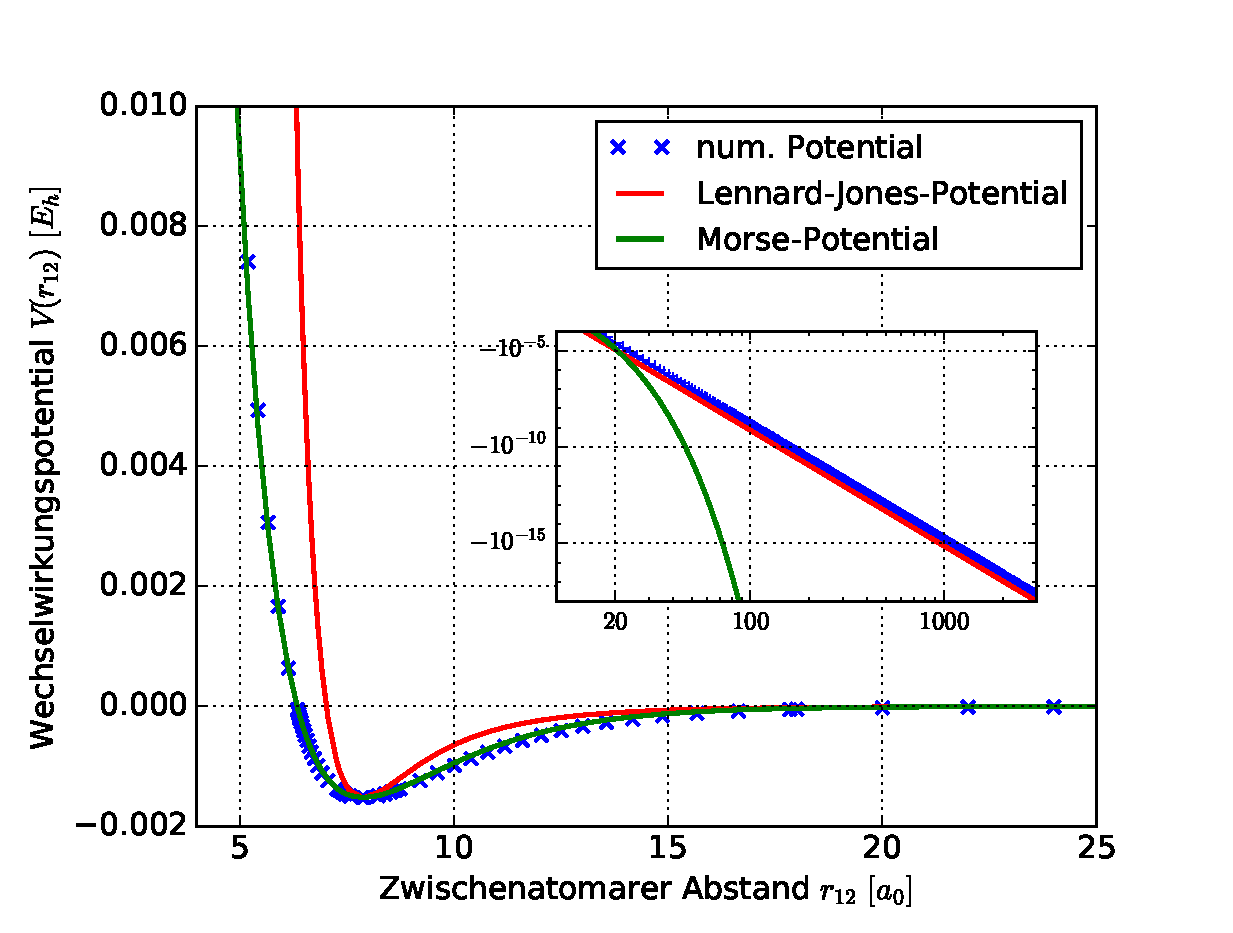
\includegraphics[scale=0.7]{WW.eps}
%	%	\vspace*{-10mm}
%	\caption{Dargestellt ist ein numerisches Potential (blau, gekreuzt) eines 
%	angeregten Tripletzustandes des $^7$Li$^7$Li Systems und 
%	zwei 
%	Näherungsfunktionen: das Morse-Potential (grün) und das 
%	Lennard-Jones-Potential (rot). Im Sub-Plot sieht man das Verhalten für 
%	größere Abstände. Für die Parameter $D_e$ (Dissoziationsenergie) und $R_m$ 
%	(Lage des Minimuns) ist der Tiefpunkt der 
%	numerischen Kurve benutzt worden. Der Exponent des MRPs 
%	wird zu 
%	$a_\text{st}=0.45$ 
%	gewählt.}
%	%\vspace{2mm} %\hrule 
%	\label{pic:Pot} 
%\end{figure}
%
In \ref{pic:Pot} ist zu sehen, dass das MRP im Bereich von 5-20 $a_0$ eine sehr 
gute Näherung 
darstellt, wogegen das LJP in diesem Bereich kaum dem numerischen Potential 
folgt. Für Abstände größer als 20 $a_0$ hingegen fällt das 
MRP deutlich zu 
schnell ab. Schon bei einem Abstand von ungefähr 100 $a_0$ erreicht es schon 
die Rechnergenauigkeit und wird auf 0 gerundet. Das LJP nähert sich dagegen der 
numerischen Kurve weiter an und 
folgt der Kurve 
über mehrere Größenordnungen des Abstandes. Lediglich ein leichter Off-set ist 
zu erahnen. An dieser Stelle sei erwähnt, dass die hier 
dargestellte Näherung 
nur durch optische Anpassung gewonnen wird. Es ist zu 
erwarten, dass eine 
numerische Anpassung (Fit) ein besseres Ergebnis auf Kosten 
einer 
Nichtübereinstimmung im Minima liefern kann.  \\

Das MRP besitzt den großen Vorteil einer vollständigen Beschreibung und 
Berechnung ohne den Bedarf einer Renormierung. Dagegen beschreibt das LJP die 
physikalische Gegebenheit besser und für große Abstände auch quantitativ 
genauer. Mithilfe des freien Parameters im Exponenten 
kann jedoch das MRP die Kurve nahe am Ursprung besser beschreiben. \\

Ziel der Betrachtung ist es, die Bemühung einer Renomierung des bekannten 
$\delta$-Pseudopotentials als Wechselwirkungspotential zu umgehen, indem ein 
realistisches Potential verwendet wird. Erhofft wird eine bessere Berechnung 
mittels CI von ultrakalten Gasen. Durch Nutzung des LJP und 
des 
Algorithmus kann zwar ein realistisches bzw. 
realistischeres\footnote{da das 
LJP dennoch eine Näherungsfunktion ist} Potential als das 
$\delta$-Potential 
verwendet werden, jedoch auf Kosten einer neuen 
Renormierung\footnote{Renormierung der Basisintegrale}. Dementsprechend 
erfüllt das LJP nicht ganz die erwarteten Eigenschaften. 
Dagegen ist das MRP 
mathematisch angenehmer und es ist keine Renormierung nötig. \\
Das MRP ist ebenfalls ein realistischeres Wechselwirkungspotential als das 
$\delta$-Potential, auch wenn es für große Abstände deutlich zu schnell 
abfällt. 
Dennoch soll es möglich sein, die relevanten Eigenschaften 
mittels MRP 
darzustellen und herauszufinden, ob eine CI-Rechnung 
prinzipiell möglich sei 
und ob diese eine Verbesserung liefere. Das MRP divergiert 
zwar nicht in 0, 
nimmt aber sehr große Werte an. Es kann daher passieren, dass im Rahmen der 
Integration zwar Ergebnisse produziert werden, diese aber unphysikalisch groß 
sind. Dieses Verhalten muss durch geeignete Wahl der Basisfunktionen der 
CI-Rechnung berücksichtigt werden.   \\

Weiterhin sei hier erwähnt, dass es auch Mischformen dieser Potentiale gibt. 
Vorstellbar ist, dass das Potential
%
\begin{align}
V\propto e^{-a_\text{st}\cdot r}-\rl{\frac{R_m}{r}}^6 \quad,
\end{align}
%
auch (modifiziertes) Buckingham-Potential genannt (siehe z.B. in \cite{av:2b} 
oder 
\cite{av:3b}), eine noch bessere 
Beschreibung über den gesamten Bereich der Abstände liefert und die guten 
Eigenschaften beider Potentiale vereint. Ohne weitere Untersuchung kann auf 
zwei Tatsachen hingewiesen werden: Zum einen muss auch dieses 
Potential für 
einige Fälle im Rahmen des oben beschriebenen Algorithmus renormiert werden, 
jedoch seltener als das LJP. Zum anderen 
beinhaltet dieses Potential den $\frac{1}{r^6}$ -Term und wird daher die 
Eigenschaft des LJP erben, sodass große Abstände gut 
beschrieben werden können.
%
%
%
% usw.

%-Anhang----------------------------------------------------------

\appendix

%-Literaturverzeichnis--------------------------------------------

%\nocite{*}
%die Verwendung von bibtex ist Pflicht!!!
\bibliography{bib/bibliography}
\bibliographystyle{plaindin}        %bzw.plain, unsrtdin, alphadin, abbrvdin, 
%siam
%plaindin

%-Kapitel des Anhangs---------------------------------------------

%\chapter{Schlegel-Koeffizienten und Kugelflächenfunktionen}
\label{sec:AnhangA:Schlegel}
In diesem Abschnitt sollen relevante Definitionen und 
Konventionen zur Transformation von kartesischen Ableitungen 
in sphärische Ableitungen nach Abschnitt 
\ref{sec:Hobson_schlegel} unter Zuhilfenahme der 
Schlegel-Koeffizienten und  des Hobson-Theorems angebracht 
werden. Es sei darauf hingewiesen, dass die Bedeutung der 
hier verwendeten Variablen von den in der restlichen Arbeit abweichen.  
Zunächst ist aus \cite{av:4a} bekannt, dass die 
Transformation von sphärischen in kartesische GTOs durch 
%
\begin{align}%\nonumber
%r^{l-n}\tilde{N}(n)\cdot r^n\cdot Y^l_m\cdot e^{-ar^2} 
%&=\sum_{l_x+l_y+l_z=l}^{} c(l,m,l_x,l_y,l_z)\cdot 
%N(l_x,l_y,l_z,a)\cdot x^{l_x}y^{l_y}z^{l_z}
%\cdot e^{-ar^2}\\
%\Leftrightarrow
\tilde{N}(l,a)\cdot Y^l_m 
&=\sum_{l_x+l_y+l_z=l}^{} c(l,m,l_x,l_y,l_z)\cdot 
N(l_x,l_y,l_z,a)\cdot x^{l_x}y^{l_y}z^{l_z}
\end{align}
%
gegeben ist. Hierbei sind $\tilde{N}$ und $N$ 
Normierungskonstanten und c die Schlegel-Koeffizienten, die 
durch
%
\begin{align}\nonumber
c(l,m,l_x,l_y,l_z)&=(-1)^{\frac{|m|+m}{2}}\cdot 
\sqrt{\frac{2l+1}{4\pi}\frac{(l-|m|)!}{(l+|m|)!}}\cdot 
\frac{1}{2^ll!}\cdot \\\nonumber
&\cdot 
\sum_{p=0}^{\frac{l-|m|}{2}}\binom{l}{p}\binom{p}{j}\cdot 
\frac{(-1)^p(2l-2p)!}{(l-|m|-2p)!}\cdot\\
&\cdot 
\sum_{k=0}^{j}\binom{j}{k}\binom{|m|}{l_x-2k}(\text{sign}(m)\cdot
 i)^{|m|-l_x+2k}
\end{align}
%
%clm[l_, m_, lx_, ly_, lz_] := Module[{js, val},
%If[lx + ly + lz != l, Return[0]];
%js = (lx + ly - Abs[m])/2;
%If[IntegerQ[js] == False, Return[0]];
%val = (-1)^((Abs[m] + m)/
%2) Sqrt[(2 l + 1)/(4 Pi) (l - Abs[m])!/(l + Abs[m])!]/(2^
%l l!) 
%Sum[
%Binomial[l, i] Binomial[i, js] (-1)^
%i (2 l - 2 i)!/(l - Abs[m] - 2 i)! 
%Sum[
%Binomial[js, k] Binomial[Abs[m], 
%lx - 2 k] (I Sgn2[m])^(Abs[m] - lx + 2 k), {k, 0, js}]
%, {i,0, (l - Abs[m])/2}];
%Return[val];
%]
%
gegeben sind. Hierbei ist $i$ die komplexe Einheit und 
$j:=(l_x+l_y-|m|)/2$. Weiterhin muss gelten, dass 
\begin{enumerate}
	\item ein 
	Binomialkoeffizient mit $\binom{a}{b}=0$ ausgewertet wird, falls b>a oder 
	b<0	ist,
	\item der Koeffizient c=0 gesetzt wird, falls $j\notin\mathbb{N}_0$ 
	oder $l\neq l_x+l_y+l_z$ ist,
	\item sign definiert ist als sign(m):=$\begin{cases}
	1 & , m\geq0\\
	-1 & , m<0
	\end{cases}\qquad$ .
\end{enumerate}
%
Die komplexen Kugelflächenfunktionen $Y^l_m$ sind definiert 
durch
%
\begin{align}
Y^l_m(\phi,\theta):=\sqrt{\frac{2l+1}{4\pi}\frac{(l-|m|)!}{(l+|m|)!}}\cdot
 e^{i m \phi} \cdot P^{m}_l(\cos(\theta))
\end{align}
%
mit den assoziierten Legendre-Polynomen
%
\begin{align}
P^m_l(\cos(\theta)):=\frac{(-1)^m}{2^ll!}(1-\cos^2(\theta))^{\frac{m}{2}}\cdot
\frac{\text{d}^{l+m}}{\text{d}\cos(\theta)^{l+m}}(\cos^2(\theta)-1)^l\qquad.
\end{align}
%
Es sei auf die Eigenschaft%en 
%
\begin{align}
%P^{-|m|}_l&=(-1)^m\frac{(l-|m|)!}{(l+|m|)!} P^{|m|}_l\quad,\\
Y^{-|m|}_l&=(-1)^m \rl{Y^{|m|}_l}^*
\end{align}
%
hingewiesen wodurch nur assoziierte Legendre-Polynome mit $m\geq0$ berechnet 
werden müssen \cite{b:4a}. Wie in 
\cite{av:4a} angedeutet und mit den Autoren von \cite{av:1a} 
besprochen ist, kann die reelle Version durch die Definition 
von
%
\begin{align}
c_r(l,m,l_x,l_y,l_z):=\begin{cases}
\frac{1}{\sqrt{2}}\cdot 
\left[c(l,-|m|,l_x,l_y,l_z)+(-1)^m\cdot 
c(l,|m|,l_x,l_y,l_z)\right]& , m>0 \\
c(l,0,l_x,l_y,l_z) & , m=0 \\
\frac{i}{\sqrt{2}}\cdot 
\left[c(l,-|m|,l_x,l_y,l_z)-(-1)^m\cdot 
c(l,|m|,l_x,l_y,l_z)\right]& , m<0
\end{cases}
\end{align}
%
und unter Verwendung der soliden reellen 
Kugelflächenfunktionen
%
\begin{align}
Z_{l,m}(\text{r},\theta,\phi):&=\begin{cases}
r^l\cdot\frac{1}{\sqrt{2}}\left[Y^{-|m|}_l+(-1)^m\cdot 
Y^{|m|}_l\right] & , m>0\\
r^l \cdot Y^0_l & , m=0 \\
r^l\cdot\frac{i}{\sqrt{2}}\left[Y^{-|m|}_l-(-1)^m\cdot 
Y^{|m|}_l\right]& , m<0
\end{cases}\\
&=r^l\cdot\begin{cases}
(-1)^m \cdot  
\sqrt{2}\sqrt{\frac{2l+1}{4\pi}\frac{(l-|m|)!}{(l+|m|)!}}\cdot
P^{|m|}_l(\cos(\theta))\cdot \cos(|m|\cdot \phi)& , m>0\\
\sqrt{\frac{2l+1}{4\pi}}\cdot P^{0}_l(\cos(\theta))&, m=0\\
(-1)^m\cdot \sqrt{2} 
\sqrt{\frac{2l+1}{4\pi}\frac{(l-|m|)!}{(l+|m|)!}}\cdot P^{|m|}_l(\cos(\theta)) 
\cdot \sin(|m|\cdot \phi) &, m<0
\end{cases}
\end{align}
%
zu 
%
\begin{align}
Z_{l,m}=\sum_{l_x=0}^{l}\sum_{l_y=0}^{(l-l_x)}\sum_{l_z=0}^{(l-l_x-l_y)}c_r\cdot
 x^{l_x}\cdot y^{l_y}\cdot z^{l_z}
\end{align}
%
bestimmt werden. Die reelle Rücktransformation kann durch 
Berechnung der Überlappmatrix bewerkstelligt werden. Es 
ergibt sich Formel \ref{eq:def:c_koef}
%
\begin{align*}\nonumber
c^{-1}_r(l,m,l_x,l_y,l_z)&=\frac{2}{\Gamma\rl{\frac{l_x+l_y+l_z+l+3}{2}}} 
\ \cdot \\ 
&\cdot  \sum_{a+b+c\leq l} \ _rc_{l_xl_yl_z}^{lm}\cdot 
\Gamma\rl{\frac{1+l_x+a}{2}}\cdot 
\Gamma\rl{\frac{1+l_y+b}{2}}\cdot \Gamma\rl{\frac{1+l_z+c}{2}}
\end{align*}
%
und \ref{eq:trafo_c-1}
%
\begin{align*}
x^{l_x}y^{l_y}z^{l_z} = \sum_{l=0}^{l_{max}}\sum_{m=0}^l 
c^{-1}(l,m,l_x,l_y,l_z)\cdot r^{l_{max}-l} Z_{lm}(\textbf{r})\quad,
\end{align*}
 wobei die Summe 
$\sum_{a+b+c\leq 
l}^{}$ die Bedeutung 
$\sum_{a=0}^{l}\sum_{b=0}^{l-a}\sum_{c=0}^{l-a-b}$ hat. Weiterhin wird in 
\cite{av:9a} die Beobachtung hinzugefügt, dass $c^{-1}\equiv0$ ist, falls 
$l_\text{max}-l$ ungerade ist.  Aus 
Vollständigkeitsgründen sollte erwähnt sein, dass zur 
numerischen Berechnung von $c_r$ die Fälle für $m>0$ und 
geradem $(|m|-l_x)$, $m<0$ zu ungeradem $(|m|-l_x)$ und $m=0$ zu 
geradem $l_x$ unterschiedet werden muss. In allen anderen 
Fällen ist die Summe über k identisch Null.


  
%\chapter{Ergänzung zu den T-Integralen}
\label{sec:AnhangB:T_Integral}
In diesem Abschnitt soll zum Einen die korrigierte Rechnung 
zur Formel \ref{eq:korr_T_1} detaillierter gezeigt werden und 
zum Anderen entscheidende Formeln für die Berechnung von 
$\omega_0$ und $\omega_1$ gegeben werden, da auch diese in 
\cite{av:1a2} einen Tippfehler enthalten. Wie oben schon 
angefangen, soll $T_1^\pm(x)$ berechnet werden. Es gilt 
\begin{align*}
T_1^\pm (x)=& \mathcal{R}\int_{0}^{\infty} \frac{dz}{z} \ 
e^{\pm z - xz^2}\\
\overset{\text{part. Integration}}{=}& 
\mathcal{R}\log(z)e^{\pm 
z-xz^2}|_0^\infty - \int_{0}^{\infty}\log(z)e^{\pm z-xz^2} 
\cdot (\pm 1-2xz) \quad,
\end{align*}
wobei nun die Randterme durch das Renormierungsschema 
entfallen. Es folgt 
\begin{align*}
T_1^\pm(x) &= \mp \int_{0}^{\infty}\log(z)e^{\pm z-xz^2}\ dz 
+ 2\cdot x\int_{0}^{\infty} z\ \log(z)e^{\pm z-xz^2} \ dz 
\quad.
\end{align*}
Wird mit 
\begin{align*}
z&=\frac{u}{\sqrt{x}}\\
dz&=\frac{1}{\sqrt{x}} \ du \\
x\cdot z^2&=u^2
\end{align*} 
substituiert, folgt
\begin{align*}
T_1^\pm(x)&=\mp \frac{1}{\sqrt{x}}\int_{0}^{\infty}du\ 
\log(\frac{u}{\sqrt{x}}) e^{\pm\frac{u}{\sqrt{x}}-u^2 }+ 
2x\frac{1}{\sqrt{x}}\int_{0}^{\infty}du\ 
\log(\frac{u}{\sqrt{x}})\cdot \frac{u}{\sqrt{x}}\cdot 
e^{\pm\frac{u}{\sqrt{x}}-u^2 }\\
&=\mp \frac{1}{\sqrt{x}}\int_{0}^{\infty}du\ 
\log(\frac{u}{\sqrt{x}}) e^{\pm\frac{u}{\sqrt{x}}-u^2 }+ 
2\int_{0}^{\infty}du\ \log(\frac{u}{\sqrt{x}})\cdot u\cdot 
e^{\pm\frac{u}{\sqrt{x}}-u^2 }\\
&=\mp \frac{1}{\sqrt{x}}\int_{0}^{\infty}du\ \log(u) 
e^{\pm\frac{u}{\sqrt{x}}-u^2 }
\pm  \frac{\log(\sqrt{x})}{\sqrt{x}}\int_{0}^{\infty}du\ 
e^{\pm\frac{u}{\sqrt{x}}-u^2 }
+ 2\int_{0}^{\infty}du\ \log(u)\cdot u\cdot 
e^{\pm\frac{u}{\sqrt{x}}-u^2 }\\
&\ \ \ \ \ -2 \log(\sqrt{x})\int_{0}^{\infty}du\cdot u\cdot 
e^{\pm\frac{u}{\sqrt{x}}-u^2 }\qquad.
\end{align*}
Im letzten Schritt wurde 
$\log(\frac{a}{b})=\log(a)-\log(b)$ für a,b$\in\mathbb{R}^+$ 
verwendet. Im Vergleich zu den Definitionen \ref{eq:def:omega} von 
$\omega_k(\pm\frac{1}{\sqrt{x}})$ ist zu sehen, dass
\begin{align*}
T_1^\pm(x)&= \mp \frac{1}{\sqrt{x}} \omega_0(\pm 
\frac{1}{\sqrt{x}}) + 2\omega_1(\pm\frac{1}{\sqrt{x}}) \\
& \pm \log(\sqrt{x})\int_{0}^{\infty}\frac{du}{\sqrt{x}}\ 
e^{\pm\frac{u}{\sqrt{x}}-u^2 }
-2 \log(\sqrt{x})\int_{0}^{\infty}du\cdot u\cdot 
e^{\pm\frac{u}{\sqrt{x}}-u^2 }
\end{align*}
gilt. Für die letzten beiden Integrale kann man abermals 
substituieren mit  
$z=\frac{u}{\sqrt{x}},\ du=\sqrt{x}dz$ und erhält
\begin{align}
\int_{0}^{\infty}dz \ e^{\pm z -x z^2} &=T_0^\pm(x)= 
\sqrt{\frac{\pi}{4x}}e^{\frac{1}{4x}}\left[1\pm 
\text{Erf}\rl{\frac{1}{2\sqrt{x}}}\right]\\
\int_{0}^{\infty}dz\ z\cdot e^{\pm z -x z^2}&=\frac{1}{2x}\pm 
\frac{\sqrt{\pi}e^{\frac{1}{4x}}}{4x^{\frac{3}{2}}}\cdot 
\left[1\pm \text{Erf}\rl{\frac{1}{2\sqrt{x}}}\right]\quad.
\end{align}
Für $T_1^\pm(x)$ folgt dann
\begin{align*}
T_1^\pm(x)&= \mp \frac{1}{\sqrt{x}} \omega_0(\pm 
\frac{1}{\sqrt{x}}) + 2\ \omega_1(\pm\frac{1}{\sqrt{x}}) \\
& \pm \log(\sqrt{x})\cdot 
\sqrt{\frac{\pi}{4x}}e^{\frac{1}{4x}}\left[1\pm 
\text{Erf}\rl{\frac{1}{2\sqrt{x}}}\right]\\
&-2\log(\sqrt{x})\cdot x\cdot \biggl\{  
\frac{1}{2x}\pm 
\frac{\sqrt{\pi}e^{\frac{1}{4x}}}{4x^{\frac{3}{2}}}\cdot 
\left[1\pm \text{Erf}\rl{\frac{1}{2\sqrt{x}}}\right]
\biggr\}\quad,
\end{align*}
was nichts anderes ist als
\begin{align}\nonumber
T_1^\pm(x)&= \mp \frac{1}{\sqrt{x}} \omega_0(\pm 
\frac{1}{\sqrt{x}}) + 2\ \omega_1(\pm\frac{1}{\sqrt{x}}) 
\\\nonumber
& \pm \log(\sqrt{x})\cdot 
\sqrt{\frac{\pi}{4x}}e^{\frac{1}{4x}}\\\nonumber
& +\log(\sqrt{x})\cdot 
\sqrt{\frac{\pi}{4x}}e^{\frac{1}{4x}}\text{Erf}\rl{\frac{1}{2\sqrt{x}}}\\\nonumber
& -\log(\sqrt{x})\\\nonumber
& \mp\log(\sqrt{x})\cdot 
\sqrt{\frac{\pi}{4x}}e^{\frac{1}{4x}}\\\nonumber
& -\log(\sqrt{x})\cdot 
\sqrt{\frac{\pi}{4x}}e^{\frac{1}{4x}}\text{Erf}\rl{\frac{1}{2\sqrt{x}}}\\
%
T_1^\pm(x)&= \mp \frac{1}{\sqrt{x}} \omega_0(\pm 
\frac{1}{\sqrt{x}}) + 2\ 
\omega_1(\pm\frac{1}{\sqrt{x}})-\frac12 \log(x)\quad.
\end{align}
$\omega_0$ und $\omega_1$ können mithilfe von
%
\begin{align}\label{omega}
\omega_k(x)=\begin{cases}
\sum_{n=0}^{\infty}\frac{(-x)^n}{n!}\frac{1}{4}\Gamma\rl{\frac{n+1}{2}}
\psi_d\rl{\frac{n+1}{2}}&,
k=0\\
\sum_{n=0}^{\infty}\frac{(-x)^n}{n!}\frac{1}{4}\Gamma\rl{\frac{n}{2}+1}
\psi_d\rl{\frac{n}{2}+1}&,
k=1\\
\end{cases}
\end{align}
%
berechnet werden. $\psi_d$ ist dabei die Diagamma-Funktion 
(vergleiche \cite{av:1a2}). Hierbei fehlt in \cite{av:1a2} im 
Vergleich zu \ref{omega} der Faktor $\frac{1}{4}$.
%\chapter{Abstandsvariation}
\label{sec:AnhangC:Tests}
\vspace{-15mm}
\begin{table}[H] \centering \scriptsize
	\caption{Genauigkeitstest der Subroutine 
	\texttt{gto\_int} 
		zu verschiedenen Abständen am Beispiel des Orbitals (0,0,1) mit 
		a=c=0,001 und den analytischen Ergebnis 
		$I_\text{Norm}=$9,6894614625937E+11 . Vergleiche mit dem Abschnitt 
		\ref{sec:var.Abstand_norm}.
		} \vspace{0.2cm}
	\begin{threeparttable} 
		\begin{tabular}{c||c||c}
			$A_x$&  $I_\text{gto\_int}$      
			&$\left|\frac{I_\text{gto\_int}-I_\text{Norm}}{I_\text{Norm}}\right|$
			\\ \hline\hline
1   & 9,6894614626032E+11 & 9,85E-13 \\
11  & 9,6894614625937E+11 & 3,15E-15 \\
21  & 9,6894614625937E+11 & 2,77E-15 \\
31  & 9,6894614625937E+11 & 1,01E-15 \\
41  & 9,6894614625937E+11 & 8,82E-16 \\
51  & 9,6894614625937E+11 & 3,91E-15 \\
61  & 9,6894614625937E+11 & 4,41E-15 \\
71  & 9,6894614625938E+11 & 5,42E-15 \\
81  & 9,6894614625937E+11 & 4,28E-15 \\
91  & 9,6894614625938E+11 & 1,45E-14 \\
101 & 9,6894614625936E+11 & 1,36E-14 \\
111 & 9,6894614625939E+11 & 1,89E-14 \\
121 & 9,6894614625939E+11 & 1,88E-14 \\
131 & 9,6894614625964E+11 & 2,83E-13 \\
141 & 9,6894614626146E+11 & 2,16E-12 \\
151 & 9,6894614626988E+11 & 1,09E-11 \\
161 & 9,6894614629157E+11 & 3,32E-11 \\
171 & 9,6894614632269E+11 & 6,53E-11 \\
181 & 9,6894614634201E+11 & 8,53E-11 \\
191 & 9,6894614633419E+11 & 7,72E-11 \\
201 & 9,6894614631126E+11 & 5,36E-11 \\
211 & 9,6894614708224E+11 & 8,49E-10 \\
221 & 9,6894629512726E+11 & 1,54E-07 \\
231 & 9,6895889515523E+11 & 1,32E-05 \\
241 & 9,6946851337730E+11 & 5,39E-04 \\
251 & 9,7958928980603E+11 & 1,10E-02 \\
261 & 9,3629351150524E+11 & 3,37E-02 \\
271 & 8,2167349128430E+11 & 1,52E-01 \\
281 & 2,6272356631903E+12 & 1,71E+00 \\
291 & 3,9536166069396E+12 & 3,08E+00 \\
301 & 4,8945748135127E+11 & 4,95E-01 \\
311 & 2,6091793452050E+12 & 1,69E+00 \\
321 & 1,0196033794039E+12 & 5,23E-02 \\
331 & 7,3362621700278E+10 & 9,24E-01 \\
341 & 4,8575674930267E+10 & 9,50E-01 \\
351 & 2,2056326063642E+09 & 9,98E-01 \\
361 & 4,5359047541451E+08 & 1,00E+00 \\
371 & 1,2285475976013E+07 & 1,00E+00 \\
381 & 8,9681048786680E+05 & 1,00E+00 \\
391 & 1,4147366231558E+04 & 1,00E+00 \\
401 & 4,0208707893439E+02 & 1,00E+00 \\
411 & 7,1286774514250E+00 & 1,00E+00
		\end{tabular}
		%		\begin{tablenotes}
		%	\item[I] 
		%		\end{tablenotes}
	\end{threeparttable}
	\label{tab:norm:abstand_2}
\end{table}
%
%usw.

%-Abkuerzungen*---------------------------------------------------

%\chapter*{Abk�rzungen}


\begin{tabular}{ll}
 Abk�rzung & Erkl�rung    \\
 \hline
      z.B. & zum Beispiel \\
\end{tabular}



%-Danksagung*-----------------------------------------------------

%%-Danksagung------------------------------------------------------

\chapter*{Danksagung}
Hier folgt dann eine Danksagung.


%-Lebenslauf*-----------------------------------------------------

%\chapter*{Lebenslauf}

%

\begin{tabular}{ll}

Name: & \dcauthorname  \dcauthorsurname \\

10.1994--09.1995 & Studium an der Humboldt-Universit"at zu Berlin \\

 & in der Fachrichtung Biologie\\

10.1995--11.1996 & Wissenschaftliche Mitarbeiterin an \\

 & der Humboldt-Universit"at zu Berlin,\\

 & Lehrstuhl Prof. XY, \\

 & Institut f"ur Biologie\\

\end{tabular}


%-Selbständigkeiterklärung--------------------------------------

\section*{Selbst\"andigkeitserkl\"arung}


Ich erkl\"are hiermit, dass ich die vorliegende Arbeit selbst\"andig verfasst und 
noch nicht f\"ur andere Pr\"ufungen eingereicht habe. S\"amtliche Quellen 
einschlie\ss lich Internetquellen, die unver\"andert oder abgewandelt wiedergegeben 
werden, insbesondere Quellen f\"ur Texte, Grafiken, Tabellen und Bilder, sind als 
solche kenntlich gemacht. Mir ist bekannt, dass bei Verst\"o\ss en gegen diese 
Grunds\"atze ein Verfahren wegen T\"auschungsversuchs bzw. T\"auschung eingeleitet 
wird.\\[3cm]
%
\includegraphics{unterschrift_richard}\\ 
Berlin, \dcdatesubmitted

%-----------------------------------------------------------------

\end{document}
